\documentclass[12pt]{article}
\usepackage[utf8]{inputenc}
\usepackage{amsmath,amsthm,amsfonts,amssymb}
\usepackage{tikz}
\usepackage{subfig}
\usepackage[english]{babel}
\usepackage{capt-of}
\usepackage{tabularray}
\newtheorem{theorem}{Theorem}
\usetikzlibrary{calc}
\usetikzlibrary{shapes}
\usepackage{hyperref}
%might be unnecessary
\usepackage{doi}

%bibliography CMDS

\usepackage{cite}


%%% With amsthm package, creates environments for nicely formatted,
%%% labeled, and numbered propositions, etc.
\theoremstyle{plain}
\newtheorem{thm}{Theorem}
\newtheorem{lemma}[thm]{Lemma}
\newtheorem{prop}[thm]{Proposition}
\newtheorem{conj}[thm]{Conjecture}
\newtheorem{cor}[thm]{Corollary}
\newtheorem{claim}[thm]{Claim}
\newtheorem{fact}[thm]{Fact}

\theoremstyle{definition}
\newtheorem{eg}[thm]{Example}
\newtheorem{defn}[thm]{Definition}
\newtheorem{rem}[thm]{Remark}
\newtheorem{observ}[thm]{Observation}
\newtheorem{open}[thm]{Open Problem}
\newtheorem{prob.}[thm]{Problem}
\newtheorem{quest}[thm]{Question}

% I used these for making definitions and theorems, not what is above
\theoremstyle{remark}
\newtheorem{remark}[thm]{Remark}
\newtheorem{note}[thm]{Note}
\theoremstyle{definition}
\newtheorem{definition}{Definition}[section]
\newtheorem{exmp}{Example}[section]

%personal commands
\newcommand{\cell}[4]{\filldraw[gray!40] ( #1 , #2 ) rectangle ( #3 , #4 ); \draw[thick] ( #1 , #2 ) rectangle ( #3 , #4 );}

\newcommand{\lablnode}[3]{\node[shape=circle,draw=white,fill=white, inner sep=0pt,minimum size=1pt] (A) at ( #1 , #2 ) {\{#3\}};}

%disjoint union symbol code
\makeatletter
\def\moverlay{\mathpalette\mov@rlay}
\def\mov@rlay#1#2{\leavevmode\vtop{%
   \baselineskip\z@skip \lineskiplimit-\maxdimen
   \ialign{\hfil$\m@th#1##$\hfil\cr#2\crcr}}}
\newcommand{\charfusion}[3][\mathord]{
    #1{\ifx#1\mathop\vphantom{#2}\fi
        \mathpalette\mov@rlay{#2\cr#3}
      }
    \ifx#1\mathop\expandafter\displaylimits\fi}
\makeatother

\newcommand{\cupdot}{\charfusion[\mathbin]{\cup}{\cdot}}

%colored cell commands
\newcommand{\cellw}[4]{\draw[thick] ( #1 , #2 ) rectangle ( #3 , #4 );}

\newcommand{\cellred}[4]{\filldraw[red!60] ( #1 , #2 ) rectangle ( #3 , #4 ); \draw[thick] ( #1 , #2 ) rectangle ( #3 , #4 );}

\newcommand{\cellorange}[4]{\filldraw[orange!80] ( #1 , #2 ) rectangle ( #3 , #4 ); \draw[thick] ( #1 , #2 ) rectangle ( #3 , #4 );}

\newcommand{\cellyellow}[4]{\filldraw[yellow!80] ( #1 , #2 ) rectangle ( #3 , #4 ); \draw[thick] ( #1 , #2 ) rectangle ( #3 , #4 );}

\newcommand{\cellgreen}[4]{\filldraw[green!60] ( #1 , #2 ) rectangle ( #3 , #4 ); \draw[thick] ( #1 , #2 ) rectangle ( #3 , #4 );}

\newcommand{\cellpurple}[4]{\filldraw[purple!80] ( #1 , #2 ) rectangle ( #3 , #4 ); \draw[thick] ( #1 , #2 ) rectangle ( #3 , #4 );}

\newcommand{\cellpink}[4]{\filldraw[pink!80] ( #1 , #2 ) rectangle ( #3 , #4 ); \draw[thick] ( #1 , #2 ) rectangle ( #3 , #4 );}

\newcommand{\cellcyan}[4]{\filldraw[cyan!60] ( #1 , #2 ) rectangle ( #3 , #4 ); \draw[thick] ( #1 , #2 ) rectangle ( #3 , #4 );}

\newcommand{\cellblue}[4]{\filldraw[blue!60] ( #1 , #2 ) rectangle ( #3 , #4 ); \draw[thick] ( #1 , #2 ) rectangle ( #3 , #4 );}

\newcommand{\createtri}[6]{\filldraw[gray!40] ( #1 , #2 ) -- ( #3 , #4 ) -- ( #5 , #6 ) -- cycle; \draw[thick] ( #1 , #2 ) -- ( #3 , #4 ) -- ( #5 , #6 ) -- cycle;}

\newcommand{\dimer}[4]{\draw[fill=black] ( #1 , #2 ) circle (3pt);\draw[fill=black] (#3 , #4) circle (3pt);
        \draw[ultra thick] ( #1 , #2 ) -- ( #3 , #4);}
        
\newcommand{\rdimer}[4]{\draw[red,fill=red] ( #1 , #2 ) circle (3pt);\draw[red,fill=red] (#3 , #4) circle (3pt);
        \draw[ultra thick,red] ( #1 , #2 ) -- ( #3 , #4);}
        
\newcommand{\hexagon}{\mathord{\raisebox{0.6pt}{\tikz{\node[draw,scale=.75,regular polygon, regular polygon sides=6](){};}}}}

%nice quick solution
\usepackage[margin=1in]{geometry}


%doc info
\title{Minimal Inscribed Polyforms}
\author{Jack Hanke}
\date{\today}

\begin{document}

\begin{center}
    \Large
    \textbf{Minimal Inscribed Polyforms}
    
    \vspace{0.4cm}
    \large
    Jack Hanke
    
    \vspace{0.4cm}
    \large
    University of Connecticut
    
    \vspace{0.4cm}
    
    \begin{abstract}
        A polyomino is a shape in the plane constructed by joining unit squares along their edges. The question of how many polyominos there are with $n$ unit squares is a famous unsolved problem in combinatorics. This has lead many to study polyomino families, which are polyominos with additional rules that must be adhered to in construction. One such family is the minimally inscribed polyominos. This paper extends this family to other lattices, and gives novel formulae for multiple minimal inscribed polyforms.
    \end{abstract}
    
\end{center}

\section{Introduction}

A \textit{polyomino of area} $n$ is a shape in $\mathbb{Z}^2$ constructed by joining $n$ unit squares called \textit{cells} along their edges. A domino is the case $n=2$. Polyominos of area $n$ are often referred to as $n$-ominos. 

\begin{center}
    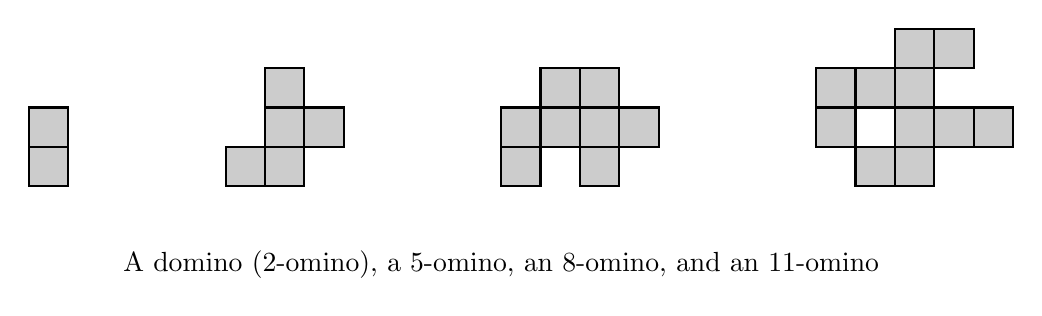
\begin{tikzpicture}
    \( \cell{0}{0}{0.5}{0.5} \)
    \( \cell{0}{0.5}{0.5}{1} \)
    
    \( \cell{2.5}{0}{3}{0.5} \)
    \( \cell{3}{0}{3.5}{0.5} \)
    \( \cell{3}{0.5}{3.5}{1} \)
    \( \cell{3}{1}{3.5}{1.5} \)
    \( \cell{3.5}{0.5}{4}{1} \)
    
    \( \cell{6}{0}{6.5}{0.5} \)
    \( \cell{6}{0.5}{6.5}{1} \)
    \( \cell{6.5}{0.5}{7}{1} \)
    \( \cell{6.5}{1}{7}{1.5} \)
    \( \cell{7}{0}{7.5}{0.5} \)
    \( \cell{7}{0.5}{7.5}{1} \)
    \( \cell{7}{1}{7.5}{1.5} \)
    \( \cell{7.5}{0.5}{8}{1} \)
    
    \( \cell{10}{0.5}{10.5}{1} \)
    \( \cell{10}{1}{10.5}{1.5} \)
    \( \cell{10.5}{0}{11}{0.5} \)
    \( \cell{10.5}{1}{11}{1.5} \)
    \( \cell{11}{0}{11.5}{0.5} \)
    \( \cell{11}{0.5}{11.5}{1} \)
    \( \cell{11}{1}{11.5}{1.5} \)
    \( \cell{11}{1.5}{11.5}{2} \)
    \( \cell{11.5}{0.5}{12}{1} \)
    \( \cell{11.5}{1.5}{12}{2} \)
    \( \cell{12}{0.5}{12.5}{1} \)
    %caption
    \node at (6,-1) (x) {A domino ($2$-omino), a $5$-omino, an $8$-omino, and an $11$-omino};
    \end{tikzpicture}
\end{center}

Polyominos are traditionally enumerated under different equivalence classes distinguished by rotational and reflective symmetries. For this paper, we will only consider the enumeration of \textit{fixed} polyominos. 

\begin{definition}\label{def:fixedpolyominos}
The class of \textit{fixed} polyominos of area $n$ consists of all possible polyominos up to translation, regardless of other symmetries.
\end{definition}

Whenever the enumeration of polyominos or polyomino families are mentioned within this paper, it can be assumed we are enumerating under the fixed equivalence class. 

Let us call the number of fixed $n$-ominos $t_n$. The first couple terms of $t_n$ for $n \geq 1$ are 

$$1,2,6,19,63,219,760,2725,9910,36446,\dots (A001168 \text{\cite{oeis}})$$

\begin{exmp}
The number of fixed $4$-ominos is $19$, colored by their appearance in the popular video game TETRIS.

\begin{center}
    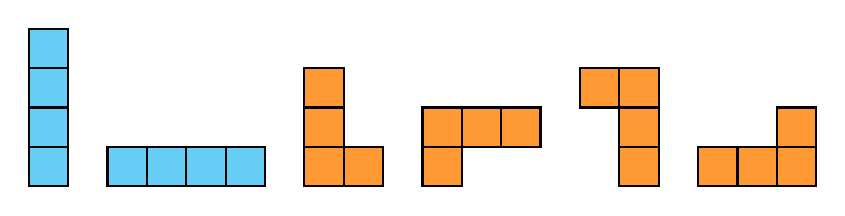
\begin{tikzpicture}
        \( \cellcyan{-1}{0}{-0.5}{0.5} \)
        \( \cellcyan{-1}{0.5}{-0.5}{1} \)
        \( \cellcyan{-1}{1}{-0.5}{1.5} \)
        \( \cellcyan{-1}{1.5}{-0.5}{2} \)
        
        \( \cellcyan{0}{0}{0.5}{0.5} \)
        \( \cellcyan{0.5}{0}{1}{0.5} \)
        \( \cellcyan{1}{0}{1.5}{0.5} \)
        \( \cellcyan{1.5}{0}{2}{0.5} \)
        
        \( \cellorange{2.5}{0}{3}{0.5} \)
        \( \cellorange{2.5}{0.5}{3}{1} \)
        \( \cellorange{2.5}{1}{3}{1.5} \)
        \( \cellorange{3}{0}{3.5}{0.5} \)
        
        \( \cellorange{4}{0}{4.5}{0.5} \)
        \( \cellorange{4}{0.5}{4.5}{1} \)
        \( \cellorange{4.5}{0.5}{5}{1} \)
        \( \cellorange{5}{0.5}{5.5}{1} \)
        
        \( \cellorange{6}{1}{6.5}{1.5} \)
        \( \cellorange{6.5}{0}{7}{0.5} \)
        \( \cellorange{6.5}{0.5}{7}{1} \)
        \( \cellorange{6.5}{1}{7}{1.5} \)
        
        \( \cellorange{7.5}{0}{8}{0.5} \)
        \( \cellorange{8}{0}{8.5}{0.5} \)
        \( \cellorange{8.5}{0}{9}{0.5} \)
        \( \cellorange{8.5}{0.5}{9}{1} \)
    \end{tikzpicture}
\end{center}
\begin{center}
    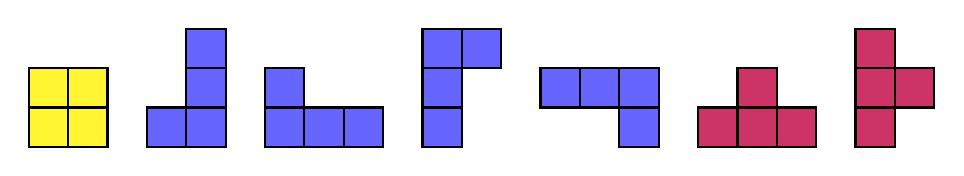
\begin{tikzpicture}
    \( \cellyellow{-1.5}{0}{-1}{0.5} \)
    \( \cellyellow{-1.5}{0.5}{-1}{1} \)
    \( \cellyellow{-1}{0}{-0.5}{0.5} \)
    \( \cellyellow{-1}{0.5}{-0.5}{1} \)
    
    \( \cellblue{0}{0}{0.5}{0.5} \)
    \( \cellblue{0.5}{0}{1}{0.5} \)
    \( \cellblue{0.5}{0.5}{1}{1} \)
    \( \cellblue{0.5}{1}{1}{1.5} \)
    
    \( \cellblue{1.5}{0}{2}{0.5} \)
    \( \cellblue{1.5}{0.5}{2}{1} \)
    \( \cellblue{2}{0}{2.5}{0.5} \)
    \( \cellblue{2.5}{0}{3}{0.5} \)
    
    \( \cellblue{3.5}{0}{4}{0.5} \)
    \( \cellblue{3.5}{0.5}{4}{1} \)
    \( \cellblue{3.5}{1}{4}{1.5} \)
    \( \cellblue{4}{1}{4.5}{1.5} \)
    
    \( \cellblue{5}{0.5}{5.5}{1} \)
    \( \cellblue{5.5}{0.5}{6}{1} \)
    \( \cellblue{6}{0}{6.5}{0.5} \)
    \( \cellblue{6}{0.5}{6.5}{1} \)
    
    \( \cellpurple{7}{0}{7.5}{0.5} \)
    \( \cellpurple{7.5}{0}{8}{0.5} \)
    \( \cellpurple{7.5}{0.5}{8}{1} \)
    \( \cellpurple{8}{0}{8.5}{0.5} \)
    
    \( \cellpurple{9}{0}{9.5}{0.5} \)
    \( \cellpurple{9}{0.5}{9.5}{1} \)
    \( \cellpurple{9}{1}{9.5}{1.5} \)
    \( \cellpurple{9.5}{0.5}{10}{1} \)
    \end{tikzpicture}
\end{center}
\begin{center}
    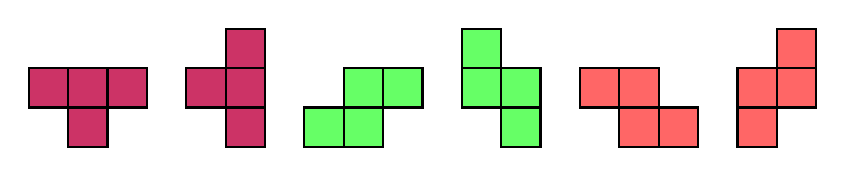
\begin{tikzpicture}
    \( \cellpurple{0}{0.5}{0.5}{1} \)
    \( \cellpurple{0.5}{0}{1}{0.5} \)
    \( \cellpurple{0.5}{0.5}{1}{1} \)
    \( \cellpurple{1}{0.5}{1.5}{1} \)

    \( \cellpurple{2}{0.5}{2.5}{1} \)
    \( \cellpurple{2.5}{0}{3}{0.5} \)
    \( \cellpurple{2.5}{0.5}{3}{1} \)
    \( \cellpurple{2.5}{1}{3}{1.5} \)
    
    \( \cellgreen{3.5}{0}{4}{0.5} \)
    \( \cellgreen{4}{0}{4.5}{0.5} \)
    \( \cellgreen{4}{0.5}{4.5}{1} \)
    \( \cellgreen{4.5}{0.5}{5}{1} \)
    
    \( \cellgreen{5.5}{0.5}{6}{1} \)
    \( \cellgreen{5.5}{1}{6}{1.5} \)
    \( \cellgreen{6}{0}{6.5}{0.5} \)
    \( \cellgreen{6}{0.5}{6.5}{1} \)
    
    \( \cellred{7}{0.5}{7.5}{1} \)
    \( \cellred{7.5}{0}{8}{0.5} \)
    \( \cellred{7.5}{0.5}{8}{1} \)
    \( \cellred{8}{0}{8.5}{0.5} \)
    
    \( \cellred{9}{0}{9.5}{0.5} \)
    \( \cellred{9}{0.5}{9.5}{1} \)
    \( \cellred{9.5}{0.5}{10}{1} \)
    \( \cellred{9.5}{1}{10}{1.5} \)
    \end{tikzpicture}
    \captionof{figure}{All $19$ fixed $4$-ominos}
    \label{fig:tetris pieces}
\end{center}
\end{exmp}

Given the simplicity of their definition, it is surprising that there is no closed formula known for $t_n$. It is known however that $t_n$ is exponential.

Klarner \cite{klarner_1967} proved that $\lim_{n \to \infty}(t_n)^{\frac{1}{n}}$ exists and has a finite value $\lambda$. Madras \cite{Madras1999APT} followed by proving that $\lim_{n \to \infty} \frac{t_{n+1}}{t_n}$ exists, and consequently is also equal to $\lambda$. This value is often referred to as Klarner's constant. The best current proven lower bound for $\lambda$ is $3.980$ \cite{Barequet2004} , and best current proven upper bound is $4.6496$ \cite{klarner_rivest_1973}.

The apparent difficulty of the problem has lead many to the study of polyomino families \cite{Gessel99onthe, BARCUCCI200562, Lin_1988}. Polyomino families add constraints on polyomino construction to introduce additional structure. One such family was introduced by Goupil, Cloutier, and Noubound \cite{10.1016/j.dam.2010.08.011} called the \textit{minimal inscribed polyominos}.

\section{Minimal Inscribed Polyominos}
\label{sec:minimals}

\begin{definition}\label{def:minimalinscribedpolyomino}
    A polyomino is \textit{minimal inscribed} when it is contained in a $w \times \ell$ rectangular lattice, where each of the four sides of the rectangle is touched by a cell of the polyomino, and the polyomino is of minimal area $w+ \ell -1$.
\end{definition}

\begin{center}
    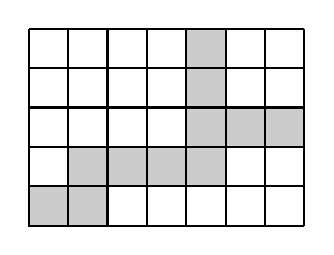
\begin{tikzpicture}[every node/.style={minimum size=.5cm-\pgflinewidth, outer sep=0pt}]
    \draw[step=0.5cm,color=black,thick] (0,0) grid (3.5,2.5);
    \( \cell{0}{0}{0.5}{0.5} \)
    \( \cell{0.5}{0}{1}{0.5} \)
    \( \cell{0.5}{0.5}{1}{1} \)
    \( \cell{1}{0.5}{1.5}{1} \)
    \( \cell{1.5}{0.5}{2}{1} \)
    \( \cell{2}{0.5}{2.5}{1} \)
    \( \cell{2}{1}{2.5}{1.5} \)
    \( \cell{2}{1.5}{2.5}{2} \)
    \( \cell{2}{2}{2.5}{2.5} \)
    \( \cell{2.5}{1}{3}{1.5} \)
    \( \cell{3}{1}{3.5}{1.5} \)
    \end{tikzpicture}
    \captionof{figure}{A minimal inscribed $11$-omino in a $7 \times 5$ lattice}
    \label{fig:ex minimally inscribed poly}
\end{center}

How many minimal inscribed polyominos are there for a given $w \times \ell$ lattice? 

\begin{theorem}[\cite{10.1016/j.dam.2010.08.011}]\label{thm:minimalsformula}
Let $s_{w,\ell}$ be the number of minimal inscribed polyominos in a given $w \times \ell$ lattice. Then $s_{w,\ell}=8\binom{w+\ell-2}{w-1} -3w\ell + 2w +2\ell-8$.
\end{theorem}

\begin{proof}
First, fix $w$ and $\ell$, and call $S$ the set of all $(w+\ell-1)$-ominos that can be inscribed in a $w \times \ell$ lattice. $S$ can be split into three distinct subsets based on the number of corners of the rectangle each polyomino touches. $S_2$ contains polyominos that contain either $2$ or $3$ corners, $S_1$ contains polyominos that contain $1$ corner, and $S_0$ contains polyominos that contain no corners. An example of each subset for the $4 \times 4$ lattice is shown in Figure \ref{fig:minimalssubsets}.

\begin{center}
    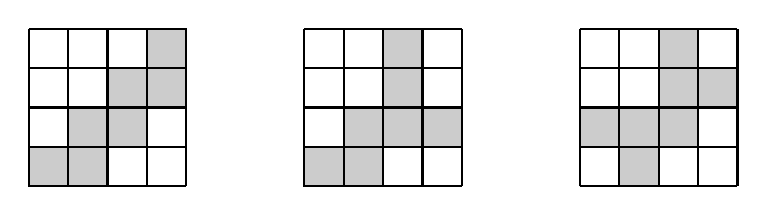
\begin{tikzpicture}[every node/.style={minimum size=.5cm-\pgflinewidth, outer sep=0pt}]
    \draw[step=0.5cm,color=black,thick] (0,0) grid (2,2);
    \( \cell{0}{0}{0.5}{0.5} \);
    \( \cell{0.5}{0}{1}{0.5} \);
    \( \cell{0.5}{0.5}{1}{1} \);
    \( \cell{1}{0.5}{1.5}{1} \);
    \( \cell{1}{1}{1.5}{1.5} \);
    \( \cell{1.5}{1}{2}{1.5} \);
    \( \cell{1.5}{1.5}{2}{2} \);
    
    \draw[step=0.5cm,color=black,thick] (3.5,0) grid (5.5,2);
    \draw[thick] (3.5,0) -- (3.5,2);
    \( \cell{3.5}{0}{4}{0.5} \);
    \( \cell{4}{0}{4.5}{0.5} \);
    \( \cell{4}{0.5}{4.5}{1} \);
    \( \cell{4.5}{0.5}{5}{1} \);
    \( \cell{5}{0.5}{5.5}{1} \);
    \( \cell{4.5}{1}{5}{2} \);
    \( \cell{4.5}{1.5}{5}{2} \);
    
    \draw[step=0.5cm,color=black,thick] (7,0) grid (9,2);
    \draw[thick] (7,0) -- (7,2);
    \( \cell{7.5}{0.5}{8}{1} \);
    \( \cell{7}{0.5}{7.5}{1} \);
    \( \cell{7.5}{0}{8}{0.5} \);
    \( \cell{8}{0.5}{8.5}{1} \);
    \( \cell{8}{1}{8.5}{1.5} \);
    \( \cell{8}{1.5}{8.5}{2} \);
    \( \cell{8.5}{1}{9}{1.5} \);
    
    \end{tikzpicture}
    \captionof{figure}{Examples of elements in $S_2, S_1$, and $S_0$ for a $4 \times 4$ lattice}
    \label{fig:minimalssubsets}
\end{center}

We then have that
$$S = S_2 \cupdot S_1 \cupdot S_0,$$

\noindent where $S_2$, $S_1$, and $S_0$ are disjoint.

\textbf{\textit{Case 1.}} We begin with $S_2$. Split $S_2$ into two subsets, $S_{T,2}$ and $S_{T,2}^c$ so that $S_{T,2} \cupdot S_{T,2}^c = S_2$. Let $S_{T,2}$ represent all polyominos that are ``T-shaped'', while $S_{T,2}^c$ will represent all polyominos that are not. Formally, the ``T-shaped'' polyominos are all polyominos that contain two adjacent corner cells and a perpendicular bar, as in the left polyomino in Figure \ref{fig:T-shaped minimals}.

\begin{center}
    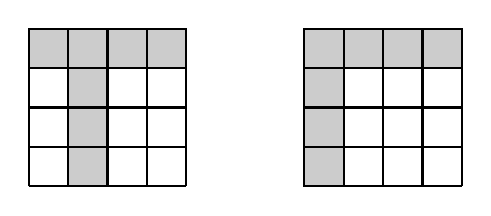
\begin{tikzpicture}[every node/.style={minimum size=.5cm-\pgflinewidth, outer sep=0pt}]
    \draw[step=0.5cm,color=black,thick] (0,0) grid (2,2);
    \( \cell{0.5}{0}{1}{0.5} \);
    \( \cell{0.5}{0.5}{1}{1} \);
    \( \cell{0.5}{1}{1}{1.5} \);
    \( \cell{0}{1.5}{0.5}{2} \);
    \( \cell{0.5}{1.5}{1}{2} \);
    \( \cell{1}{1.5}{1.5}{2} \);
    \( \cell{1.5}{1.5}{2}{2} \);
    
    \draw[step=0.5cm,color=black,thick] (3.5,0) grid (5.5,2);
    \draw[thick] (3.5,0) -- (3.5,2);
    \( \cell{3.5}{0}{4}{0.5} \);
    \( \cell{3.5}{0.5}{4}{1} \);
    \( \cell{3.5}{1}{4}{1.5} \);
    \( \cell{3.5}{1.5}{4}{2} \);
    \( \cell{4}{1.5}{4.5}{2} \);
    \( \cell{4.5}{1.5}{5}{2} \);
    \( \cell{5}{1.5}{5.5}{2} \);
    
    \end{tikzpicture}
    \captionof{figure}{Examples of elements in $S_{T,2}$, and $S_{T,2}^c$ for a $4 \times 4$ lattice}
    \label{fig:T-shaped minimals}
\end{center}

For $|S_{T,2}|$ it is easy to see that $|S_{T,2}| = 2(w-2) + 2(\ell-2) = 2w+2\ell-8$, as there is a ``T-shape'' polyomino for every edge cell.

For $|S_{T,2}^c|$, suppose the bottom left cell of the $w \times \ell$ lattice is called $(1,1)$, and the top right cell $(w,\ell)$. The number of paths from $(1,1)$ to $(w,\ell)$ is the number of ways one can make $w-1$ unit steps right and $\ell -1$ unit steps up among $w + \ell -2$ total unit steps. This gives a total of $\binom{w+\ell-2}{w-1}$ paths from $(1,1)$ to $(w,\ell)$. As we can make the same argument for corners $(1,\ell)$ and $(w,1)$, we can conclude $|S_{T,2}^c| = 2\binom{w+\ell-2}{w-1}$. This gives us $|S_2| = |S_{T,2}| + |S_{T,2}^c| = 2\binom{w+\ell-2}{w-1} +2w+2\ell-8$.

\textbf{\textit{Case 2.}} For $S_1$, suppose we choose corner $(1,1)$ and start a path to some cell $(i,j)$. Extending a path from $(i,j)$ to $(i,\ell)$ and from $(i,j)$ to $(w,j)$ creates a minimally inscribed polyomino that touches only one corner. In Figure \ref{fig:minimalssubsets}, $(i,j)=(3,1)$. Notice that $(i,j)$ must have $i \in [2,w-1]$, and $j \in [2,\ell-1]$, as otherwise the polyomino formed would have more than $1$ corner. Therefore, the total number of polyominos that touch only corner $(1,1)$ in $S_1$ is 
$$\sum_{i=2}^{w-1}\sum_{j=2}^{\ell-1} \binom{i+j-2}{i-1} = \binom{w+\ell-2}{w-1}-w-\ell+2.$$

As we can make the same argument starting with any corner, we have $|S_1| = 4\binom{w+\ell-2}{w-1}-4w-4\ell+8$

\textbf{\textit{Case 3.}} Finally, consider $S_0$. Suppose we have two cells $(i,j)$ and $(i',j')$, with $i,i' \in [2,w-1]$ and $j,j' \in [2,\ell-1]$, $i \leq i'$ and $j \leq j'$. 

\begin{center}
    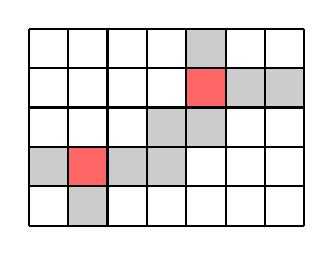
\begin{tikzpicture}[every node/.style={minimum size=.5cm-\pgflinewidth, outer sep=0pt}]
    \draw[step=0.5cm,color=black,thick] (0,0) grid (3.5,2.5);
    \( \cell{0}{0.5}{0.5}{1} \)
    \( \cell{0.5}{0}{1}{0.5} \)
    \( \cellred{0.5}{0.5}{1}{1} \)
    \( \cell{1}{0.5}{1.5}{1} \)
    \( \cell{1.5}{0.5}{2}{1} \)
    \( \cell{1.5}{1}{2}{1.5} \)
    \( \cell{2}{1}{2.5}{1.5} \)
    \( \cellred{2}{1.5}{2.5}{2} \)
    \( \cell{2}{2}{2.5}{2.5} \)
    \( \cell{2.5}{1.5}{3}{2} \)
    \( \cell{3}{1.5}{3.5}{2} \)
    
    %\node at (0.75,0.75) (x) {$i,j$};
    %\node at (1.25,-0.5) (x) {A convex polyomino};
    
    \end{tikzpicture}
    \captionof{figure}{An example of a polyomino in $S_0$ with $(i,j)$ and $(i',j')$ in red}
    \label{fig:s0 poly}
\end{center}

One can construct a path from $(i,j)$ to $(i',j')$. Next, make a path from $(i,j)$ to $(1,j)$, and a path from $(i,j)$ to $(i,1)$. Similarly, make a path from $(i',j')$ to $(w,j')$ and a path from $(i',j')$ to $(i',\ell)$. This constructs a minimal inscribed polyomino that touches no corners, as shown in Figure \ref{fig:s0 poly}. 

These polyominos can easily be enumerated by the size of the rectangle made with corners $(i,j)$, $(i,j')$, $(i',j)$, and $(i',j')$. If we suppose that $\Delta i = i'-i$, and $\Delta j = j'-j$, we can construct the following sum.

$$\sum_{\Delta i=1}^{w-2}\sum_{\Delta j=1}^{\ell-2}\binom{\Delta i+\Delta j-2}{\Delta i-1}(\ell-1- \Delta j)(w-1- \Delta i)= \binom{w+\ell-2}{w-1} -w\ell + w+\ell-2.$$

As $(i,j')$ and $(i',j)$ define the same rectangle but different polyominos, we multiply the above result by two. However, this double counts the polyominos that are built with $i=i'$ and $j=j'$. There are $(w-2)(\ell-2)$ of these polyominos, so we subtract this quantity once. Therefore $|S_0| = 2\binom{w+\ell-2}{w-1} -2w\ell + 2w+2\ell-4 - (w-2)(\ell-2) = 2\binom{w+\ell-2}{w-1} -3w\ell +4w +4\ell -8$

Combining the three subsets, we get the result.

$$|S| = |S_2|+|S_1|+|S_0|=8\binom{w+\ell-2}{w-1} -3w\ell + 2w +2\ell-8.$$

\end{proof}

Goupil et al. \cite{10.1016/j.dam.2010.08.011} proved Theorem \ref{thm:minimalsformula} similarly, only differing on the method used to enumerate case 3. The authors also enumerated the inscribed polyominos of minimal area plus 1. In a separate paper, Goupil and Cloutier enumerated the $3$-dimensional analogue of Theorem \ref{thm:minimalsformula} in \cite{Goupil2011EnumerationOM}. We chose to extend Theorem \ref{thm:minimalsformula} instead to various other lattices, and ask how many \textit{polyforms} of minimal area can be inscribed in different shapes.

\section{Extensions to Polyforms}\label{sec:extensions}

The purpose of this section will be to first generalize our definition of a polyomino to other shapes. Then we will generalize inscription in a general lattice. Finally, we will introduce notation to discuss lattices of certain sizes.

\subsection{Polyforms}

The idea behind polyforms is to construct shapes in $\mathbb{Z}^2$ with any polygons with unit side lengths.

\begin{definition}
A \textit{polyform} of area $n$ is a shape in the plane constructed by joining $n$ unit side length polygons along their edges. 
\end{definition}

\begin{center}
    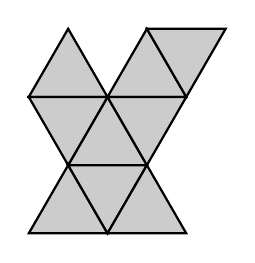
\begin{tikzpicture}
        \( \createtri{1}{0}{2}{0}{1.5}{0.866} \);
        \( \createtri{1.5}{0.866}{2.5}{0.866}{2}{1.732} \);
        \( \createtri{2}{1.732}{3}{1.732}{2.5}{2.598} \);
        \( \createtri{1}{1.732}{2}{1.732}{1.5}{2.598} \);
        \( \createtri{1.5}{0.866}{2.5}{0.866}{2}{0} \);
        \( \createtri{1.5}{0.866}{1}{1.732}{2}{1.732} \);
        \( \createtri{2.5}{0.866}{3}{1.732}{2}{1.732} \);
        \( \createtri{3}{1.732}{3.5}{2.598}{2.5}{2.598} \);
        \( \createtri{2}{0}{3}{0}{2.5}{0.866} \);
    \end{tikzpicture}
    \captionof{figure}{A polyform composed of $9$ unit triangles}
    \label{fig:polyform polyiamond}
\end{center}

Polyominos are therefore polyforms made up of squares. Other polyforms are also well studied \cite{Rastegar20, VOGE2003433}. \textit{Polyiamonds} are polyforms composed of equilateral triangles. An example can be seen in Figure \ref{fig:polyform polyiamond}. \textit{Polyhexes} are polyforms composed of regular hexagons. Most of the literature, including this paper, will focus solely on regular polygons when constructing polyforms.

There are other polyforms that have been studied \cite{Rastegar20, VOGE2003433} and have been given special names. \textit{Polyiamonds}, like the polyform in Figure \ref{fig:polyform polyiamond}, are composed of equilateral triangles. \textit{Polyhexes}, polyforms that are composed of regular hexagons, are also well studied. 

\subsection{Generalization of Inscription}
\label{sec:genofinsc}

Polyforms can be inscribed into lattices as polyominos can. For minimal inscribed polyforms it was clear what cells were considered touching a side of the rectangular lattice. In other lattices is may be less clear. For example, consider Figure \ref{fig:tri hex exmp}. 

\begin{center}
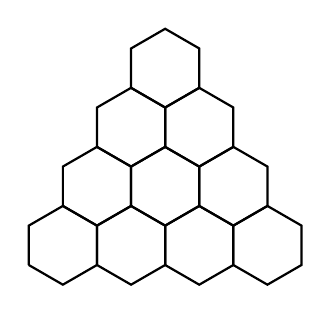
\begin{tikzpicture}
    %row 1
    \draw[thick] (0,0.25) -- (0.433,0) -- (0.866,0.25) -- (0.866,0.75) -- (0.433,1) -- (0,0.75) -- (0,0.25);
    \draw[thick] (0.866,0.25) -- (1.299,0) -- (1.732,0.25) -- (1.732,0.75) -- (1.299,1) -- (0.866,0.75) -- (0.866,0.25);
    \draw[thick] (1.732,0.25) -- (2.165,0) -- (2.598,0.25) -- (2.598,0.75) -- (2.165,1) -- (1.732,0.75) -- (1.732,0.25);
    \draw[thick] (2.598,0.25) -- (3.031,0) -- (3.464,0.25) -- (3.464,0.75) -- (3.031,1) -- (2.598,0.75) -- (2.598,0.25);

    
    %row 2
    \draw[thick] (0.433,1) -- (0.866,0.75) -- (1.299,1) -- (1.299,1.5) -- (0.866,1.75) -- (0.433,1.5) -- (0.433,1);
    \draw[thick] (1.299,1) -- (1.732,0.75) -- (2.165,1) -- (2.165,1.5) -- (1.732,1.75) -- (1.299,1.5) -- (1.299,1);
    \draw[thick] (2.165,1) -- (2.598,0.75) -- (3.031,1) -- (3.031,1.5) -- (2.598,1.75) -- (2.165,1.5) -- (2.165,1);

    
    %row 3
    \draw[thick] (0.866,1.75) -- (1.299,1.5) -- (1.732,1.75) -- (1.732,2.25) -- (1.299,2.5) -- (0.866,2.25) -- (0.866,1.75);
    \draw[thick] (1.732,1.75) -- (2.165,1.5) -- (2.598,1.75) -- (2.598,2.25) -- (2.165,2.5) -- (1.732,2.25) -- (1.732,1.75);

    
    %row 4
    \draw[thick] (1.299,2.5) -- (1.732,2.25) -- (2.165,2.5) -- (2.165,3) -- (1.732,3.25) -- (1.299,3) -- (1.299,2.5);

    
\end{tikzpicture}
\captionof{figure}{A triangle in the hexagonal lattice}
\label{fig:tri hex exmp}
\end{center}

To make it clear which cells in a given lattice belong to a side, construct the dual graph $G$ of the lattice. Then let $k$ be the number of sides chosen. Minimal inscribed polyominos have $k=4$. In Figure \ref{fig:tri hex exmp} the most obvious choice is $k=3$. After a $k$ is decided, label each vertex of $G$ with a subset of $[k]=\{1,2,\dots,k \}$, so that $\bigcup_{j \in V(G)} j = [k]$, where $V(G)$ is the vertex set of $G$. Let us call these graphs the \textit{labelled dual} of $G$.

\begin{exmp}
The lattice in Figure \ref{fig:tri hex exmp} has many possible labelled duals, one of which is shown in Figure \ref{fig:dual 4 hex}.

\begin{center}
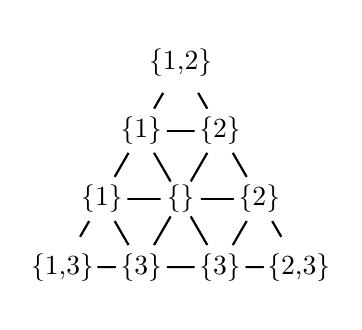
\begin{tikzpicture}
        %edges
        %\draw[thick] (0,0) -- (1,0) -- (2,0) -- (1.5,0.866) -- (1,1.732) -- (0.5,0.866);
        %\draw[thick] (0.5,0.866) -- (1.5, 0.866) -- (1,0) -- (0.5,0.866) -- (0,0);
        
        \draw[thick] (0,0) -- (3,0) -- (1.5,2.598) -- (0,0);
        %rows
        \draw[thick] (0.5,0.866) -- (2.5,0.866);
        \draw[thick] (1,1.732) -- (2,1.732);
        %big diagonals
        \draw[thick] (1,1.732) -- (2,0);
        \draw[thick] (2,1.732) -- (1,0);
        %small diagonals
        \draw[thick] (1,0) -- (0.5,0.866);
        \draw[thick] (2,0) -- (2.5,0.866);
        
        %nodes
        \( \lablnode{0}{0}{1,3} \)
        \( \lablnode{1}{0}{3} \)
        \( \lablnode{2}{0}{3} \)
        \( \lablnode{3}{0}{2,3} \)
        \( \lablnode{2}{1.732}{2} \)
        \( \lablnode{2.5}{0.866}{2} \)
        \( \lablnode{1.5}{2.598}{1,2} \)
        \( \lablnode{1}{1.732}{1} \)
        \( \lablnode{0.5}{0.866}{1} \)
        
        \( \lablnode{1.5}{0.866}{} \)
        \end{tikzpicture}
\captionof{figure}{The labelled dual of Figure \ref{fig:tri hex exmp}}
\label{fig:dual 4 hex}
\end{center}
\end{exmp}

\begin{exmp} %take out?
\label{ex:labelleddual}
We can re-frame polyomino inscription with labelled graphs. Let us call the family of $w \times \ell$ rectangles in the square lattice $\square^S_{w,\ell}$, where $\square$ designates the family is the shape of a rectangle and $S$ designates we are in a square lattice. The labelled graph considered in Theorem \ref{thm:minimalsformula} is shown below.

\begin{center}
    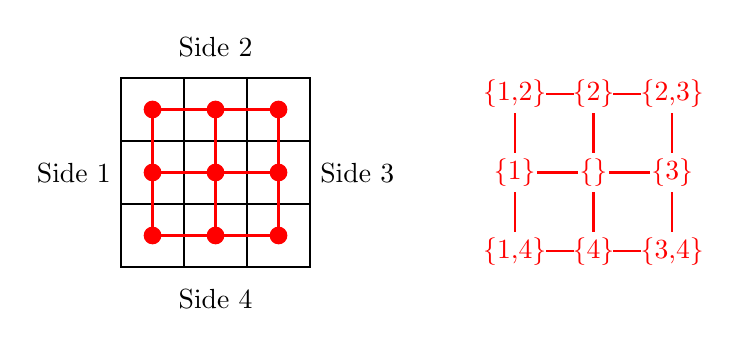
\begin{tikzpicture}
        %labels of sides
        \filldraw[black] (1.2,2.6) circle (0pt) node[anchor=center]{Side 2};
        \filldraw[black] (1.2,-0.6) circle (0pt) node[anchor=center]{Side 4};
        \filldraw[black] (-0.6,1) circle (0pt) node[anchor=center]{Side 1};
        \filldraw[black] (3,1) circle (0pt) node[anchor=center]{Side 3};
    
        %original lattice
        \draw[thick] (0,-0.2) rectangle (0.8,0.6);
        \draw[thick] (0,0.6) rectangle (0.8,1.4);
        \draw[thick] (0,1.4) rectangle (0.8,2.2);
        \draw[thick] (0.8,-0.2) rectangle (1.6,0.6);
        \draw[thick] (0.8,0.6) rectangle (1.6,1.4);
        \draw[thick] (0.8,1.4) rectangle (1.6,2.2);
        \draw[thick] (1.6,-0.2) rectangle (2.4,0.6);
        \draw[thick] (1.6,0.6) rectangle (2.4,1.4);
        \draw[thick] (1.6,1.4) rectangle (2.4,2.2);
        
        %superimposed dual
        \draw[thick,red] (0.4,0.2) -- (0.4,1.8) -- (2,1.8) -- (2,0.2) -- (0.4,0.2);
        \draw[thick,red] (0.4,1) -- (2,1);
        \draw[thick,red] (1.2,0.2) -- (1.2,1.8);
        
        \filldraw[red] (0.4,0.2) circle (3pt);
        \filldraw[red] (0.4,1) circle (3pt);
        \filldraw[red] (0.4,1.8) circle (3pt);
        \filldraw[red] (1.2,0.2) circle (3pt);
        \filldraw[red] (1.2,1) circle (3pt);
        \filldraw[red] (1.2,1.8) circle (3pt);
        \filldraw[red] (2,0.2) circle (3pt);
        \filldraw[red] (2,1) circle (3pt);
        \filldraw[red] (2,1.8) circle (3pt);
        
        
        %dual edges
        \draw[thick,red] (5,0.25) -- (5,0.75);
        \draw[thick,red] (5,1.25) -- (5,1.75);
        \draw[thick,red] (6,0.25) -- (6,0.75);
        \draw[thick,red] (6,1.25) -- (6,1.75);
        \draw[thick,red] (7,0.25) -- (7,0.75);
        \draw[thick,red] (7,1.25) -- (7,1.75);
        \draw[thick,red] (5.4,0) -- (5.75,0);
        \draw[thick,red] (6.25,0) -- (6.6,0);
        \draw[thick,red] (5.28,1) -- (5.8,1);
        \draw[thick,red] (6.2,1) -- (6.72,1);
        \draw[thick,red] (5.4,2) -- (5.75,2);
        \draw[thick,red] (6.25,2) -- (6.6,2);
        
        %dual nodes
        \filldraw[red] (5,0) circle (0pt) node[anchor=center]{\{1,4\}};
        \filldraw[red] (5,1) circle (0pt) node[anchor=center]{\{1\}};
        \filldraw[red] (5,2) circle (0pt) node[anchor=center]{\{1,2\}};
        \filldraw[red] (6,0) circle (0pt) node[anchor=center]{\{4\}};
        \filldraw[red] (6,1) circle (0pt) node[anchor=center]{\{\}};
        \filldraw[red] (6,2) circle (0pt) node[anchor=center]{\{2\}};
        \filldraw[red] (7,0) circle (0pt) node[anchor=center]{\{3,4\}};
        \filldraw[red] (7,1) circle (0pt) node[anchor=center]{\{3\}};
        \filldraw[red] (7,2) circle (0pt) node[anchor=center]{\{2,3\}};
        
    \end{tikzpicture}
    \captionof{figure}{$\square^S_{3,3}$ and the labelled dual}
    \label{fig:labelled dual of the square lattice}
\end{center}

\end{exmp}

\subsection{Minimal Inscribed Polyforms}

We can now define the polyform equivalent of inscription in the labelled dual graph.

\begin{definition}\label{def:inscribedpolyfrom}
    Suppose we have a labelled dual $G$. A given subgraph $G'$ is an \textit{inscribed polyform} in $G$ if the following condition holds.

    \begin{equation}\label{eq: condition 1 for minimals}
        \bigcup_{j \in V(G')} j = [k]
    \end{equation}
\end{definition}

Informally, condition \ref{eq: condition 1 for minimals} says that the subgraph $G'$ touches all $k$ sides. Notice that the number of vertices in an inscribed polyform of $G$ can vary. If $A$ is an inscribed polyform, then $|V(A)| \in [m(G),|V(G)|]$.  Here $m(G)$ represents the minimum number of vertices for which Condition \ref{eq: condition 1 for minimals} holds, and can range from $1$ to $|V(G)|$, depending on the structure and labelling of $G$.

\begin{exmp}
    The labelled dual in Example \ref{ex:labelleddual} is $\square^S_{3,3}$, and so $m(\square^S_{3,3}) = 5$, and so at least $5$ cells are required to touch all sides in $\square^S_{3,3}$. The $w \times \ell$ rectangular lattice has minimal area $m(\square^S_{w,\ell}) = w+\ell-1$.
\end{exmp}

Our focus is on the minimal inscribed polyforms, which are defined as follows.

\begin{definition}\label{def:minscribedpolyform}
    An inscribed polyform $A$ is \textit{minimal} if $|V(A)| = m(G)$.  
\end{definition}

Finally, we are concerned with the number of polyforms that are minimal. 

\begin{definition}
    For a labelled graph $G$, let $\rho(G)$ denote the number of minimal inscribed polyforms.
\end{definition}

\begin{exmp}
Theorem~\ref{thm:minimalsformula} gives us that $\rho(\square^S_{w,\ell}) = 8\binom{w+\ell-2}{w-1} -3w\ell + 2w +2\ell-8$.
\end{exmp}

The results of this paper will be finding expressions for $\rho(G)$ for various labelled graphs $G$.
\section{New Results on Minimal Inscribed Polyforms}\label{sec:solved}

We catalogue the known solved cases, which constitute the main new results of the paper. A summary of the results in this section can be found in the table below. %hardcoded reference

\begin{center}
    \begin{tblr}{
  colspec = {X[c,h]X[c]X[c]X[c]},
  stretch = 0,
  rowsep = 6pt,
  hlines = {black, 1pt},
  vlines = {black, 1pt},
}
  \textbf{Example Polyform} & \textbf{Notation} & $\mathbf{\rho}$\textbf{(lattice)}\\
  
  \resizebox{0.1\textwidth}{!}{%
  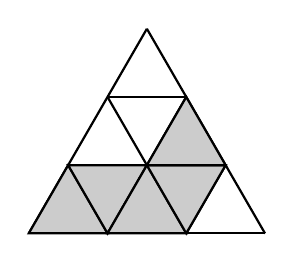
\begin{tikzpicture}
    \newcommand*\rows{3}
    \foreach \row in {0, 1, ...,\rows} {
    \draw[thick] ($\row*(0.5, {0.5*sqrt(3)})$) -- ($(\rows,0)+\row*(-0.5, {0.5*sqrt(3)})$);
    \draw[thick] ($\row*(1, 0)$) -- ($(\rows/2,{\rows/2*sqrt(3)})+\row*(0.5,{-0.5*sqrt(3)})$);
    \draw[thick] ($\row*(1, 0)$) -- ($(0,0)+\row*(0.5,{0.5*sqrt(3)})$);}
    %polyform
    \( \createtri{0}{0}{1}{0}{0.5}{0.866} \);
    \( \createtri{1}{0}{1.5}{0.866}{0.5}{0.866} \);
    \( \createtri{1}{0}{2}{0}{1.5}{0.866} \);
    \( \createtri{2}{0}{2.5}{0.866}{1.5}{0.866} \);
    \( \createtri{1.5}{0.866}{2.5}{0.866}{2}{1.732} \);
    \end{tikzpicture}%
    } 
    & $\displaystyle \triangle^{T}_n$ & $\displaystyle ((n-1)^2 +2)2^{n-2}$ \\
  \resizebox{0.1\textwidth}{!}{%
  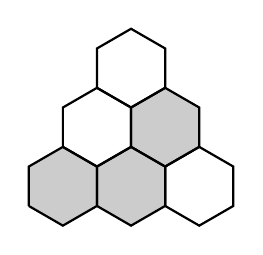
\begin{tikzpicture}
    %polyform
    %\filldraw[gray!40] (0,0.25) -- (0.433,0) -- (0.866,0.25) -- (0.866,0.75) -- (0.433,1) -- (0,0.75) -- (0,0.25);
    \filldraw[gray!40] (0,0.25) -- (0.433,0) -- (0.866,0.25) -- (1.299,0) -- (1.732,0.25) -- (1.732,0.75) -- (2.165,1) -- (2.165,1.5) -- (1.732,1.75) -- (1.299,1.5) -- (1.299,1) -- (0.866,0.75) -- (0.433,1) -- (0,0.75) -- (0,0.25);
    %\filldraw[gray!40] \draw[thick] (0.866,0.25) -- (1.299,0) -- (1.732,0.25) -- (1.732,0.75) -- (1.299,1) -- (0.866,0.75) -- (0.866,0.25);
    %\filldraw[gray!40] (1.299,1) -- (1.732,0.75) -- (2.165,1) -- (2.165,1.5) -- (1.732,1.75) -- (1.299,1.5) -- (1.299,1);
    %lattice
    \draw[thick] (0,0.25) -- (0.433,0) -- (0.866,0.25) -- (0.866,0.75) -- (0.433,1) -- (0,0.75) -- (0,0.25);
    \draw[thick] (0.866,0.25) -- (1.299,0) -- (1.732,0.25) -- (1.732,0.75) -- (1.299,1) -- (0.866,0.75) -- (0.866,0.25);
    \draw[thick] (1.732,0.25) -- (2.165,0) -- (2.598,0.25) -- (2.598,0.75) -- (2.165,1) -- (1.732,0.75) -- (1.732,0.25);
    
    \draw[thick] (0.433,1) -- (0.866,0.75) -- (1.299,1) -- (1.299,1.5) -- (0.866,1.75) -- (0.433,1.5) -- (0.433,1);
    \draw[thick] (1.299,1) -- (1.732,0.75) -- (2.165,1) -- (2.165,1.5) -- (1.732,1.75) -- (1.299,1.5) -- (1.299,1);
    
    \draw[thick] (0.866,1.75) -- (1.299,1.5) -- (1.732,1.75) -- (1.732,2.25) -- (1.299,2.5) -- (0.866,2.25) -- (0.866,1.75);
    \end{tikzpicture}%
  }
  & $\displaystyle \triangle^{H}_n$  & $\displaystyle \left( \binom{n}{2}+2 \right) 2^{n-2}$ \\
  \resizebox{0.1\textwidth}{!}{%
  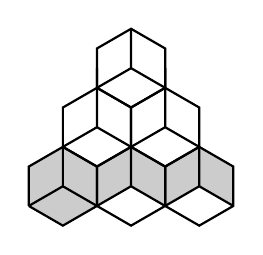
\begin{tikzpicture}
    %polyform
    \filldraw[gray!40] (0,0.25) -- (0.433,0) -- (0.866,0.25) -- (0.866,0.75) -- (0.433,1) -- (0,0.75) -- (0,0.25);
    \filldraw[gray!40] (0.866,0.25) -- (1.299,0.5) -- (1.299,1) -- (0.866,0.75) -- (0.866,0.25);
    \filldraw[gray!40] (1.732,0.25) -- (1.299,0.5) -- (1.299,1) -- (1.732,0.75) -- (1.732,0.25);
    \filldraw[gray!40] (1.732,0.25) -- (2.165,0.5) -- (2.165,1) -- (1.732,0.75) -- (1.732,0.25);
    \filldraw[gray!40] (2.598,0.25) -- (2.165,0.5) -- (2.165,1) -- (2.598,0.75) -- (2.598,0.25);
    
    %lattice
    \draw[thick] (0,0.25) -- (0.433,0) -- (0.866,0.25) -- (0.866,0.75) -- (0.433,1) -- (0,0.75) -- (0,0.25);
    \draw[thick] (0.866,0.25) -- (1.299,0) -- (1.732,0.25) -- (1.732,0.75) -- (1.299,1) -- (0.866,0.75) -- (0.866,0.25);
    \draw[thick] (1.732,0.25) -- (2.165,0) -- (2.598,0.25) -- (2.598,0.75) -- (2.165,1) -- (1.732,0.75) -- (1.732,0.25);
    
    
    \draw[thick] (0,0.25) -- (0.433,0.5) -- (0.433,1) -- (0.433,0.5) -- (0.866,0.25);
    \draw[thick] (0.866,0.25) -- (1.299,0.5) -- (1.299,1) -- (1.299,0.5) -- (1.732,0.25);
    \draw[thick] (1.732,0.25) -- (2.165,0.5) -- (2.165,1) -- (2.165,0.5) -- (2.598,0.25);
    
    
    \draw[thick] (0.433,1) -- (0.866,0.75) -- (1.299,1) -- (1.299,1.5) -- (0.866,1.75) -- (0.433,1.5) -- (0.433,1);
    \draw[thick] (1.299,1) -- (1.732,0.75) -- (2.165,1) -- (2.165,1.5) -- (1.732,1.75) -- (1.299,1.5) -- (1.299,1);
    
    \draw[thick] (0.433,1) -- (0.866,1.25) -- (0.866,2) -- (0.866,1.25) -- (1.299,1);
    \draw[thick] (1.299,1) -- (1.732,1.25) -- (1.732,2) -- (1.732,1.25) -- (2.165,1);
    
    
    \draw[thick] (0.866,1.75) -- (1.299,1.5) -- (1.732,1.75) -- (1.732,2.25) -- (1.299,2.5) -- (0.866,2.25) -- (0.866,1.75);
    
    \draw[thick] (0.866,1.75) -- (1.299,2) -- (1.299,2.5) -- (1.299,2) -- (1.732,1.75);
    \end{tikzpicture}%
  } 
  & $\displaystyle \triangle^{R}_n$  & $\displaystyle n(n+1)2^{n-2}$ \\
  \resizebox{0.1\textwidth}{!}{%
  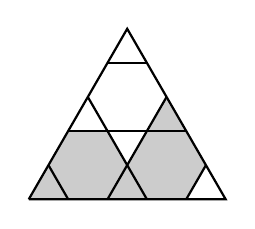
\begin{tikzpicture}
    %polyform
    \filldraw[gray!40] (0,0) -- (0.5,0) -- (0.25,0.433) -- cycle;
    \filldraw[gray!40] (1,0) -- (1.5,0) -- (1.25,0.433) -- cycle;
    \filldraw[gray!40] (1.5,0.866) -- (2,0.866) -- (1.75,1.299) -- cycle;
    
    \filldraw[gray!40] (0.25,0.433) -- (0.5,0) -- (1,0) -- (1.25, 0.433) -- (1,0.866) -- (0.5,0.866) -- (0.25,0.433);
    \filldraw[gray!40] (1.25,0.433) -- (1.5,0) -- (2,0) -- (2.25, 0.433) -- (2,0.866) -- (1.5,0.866) -- (1.25,0.433);
    
    %lattice
    \draw[thick] (0,0) -- (2.5,0) -- (1.25, 2.165) -- (0,0);
    \draw[thick] (1,1.732) -- (1.5,1.732);
    \draw[thick] (0.5,0) -- (0.25,0.433);
    \draw[thick] (2,0) -- (2.25,0.433);
    \draw[thick] (1,0) -- (1.75,1.299);
    \draw[thick] (1.5,0) -- (0.75,1.299);
    \draw[thick] (0.5,0.866) -- (2,0.866);
    \end{tikzpicture}%
  }
  & $\displaystyle \triangle^{K}_n$  & $\displaystyle \left( n^2 + 3n +\frac{10}{3} \right) 4^{n-3} - \frac{1}{3}$\\
  \resizebox{0.1\textwidth}{!}{%
  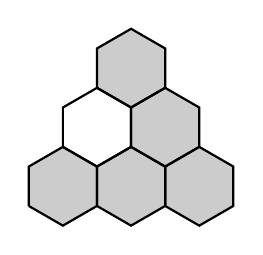
\begin{tikzpicture}
    %polyform
    %\filldraw[gray!40] (0,0.25) -- (0.433,0) -- (0.866,0.25) -- (0.866,0.75) -- (0.433,1) -- (0,0.75) -- (0,0.25);
    \filldraw[gray!40] (0,0.25) -- (0.433,0) -- (0.866,0.25) -- (1.299,0) -- (1.732,0.25) -- (1.732,0.75) -- (2.165,1) -- (2.165,1.5) -- (1.732,1.75) -- (1.299,1.5) -- (1.299,1) -- (0.866,0.75) -- (0.433,1) -- (0,0.75) -- (0,0.25);
    \filldraw[gray!40] (1.732,0.25) -- (2.165,0) -- (2.598,0.25) -- (2.598,0.75) -- (2.165,1) -- (1.732,0.75) -- (1.732,0.25);
    \filldraw[gray!40] (0.866,1.75) -- (1.299,1.5) -- (1.732,1.75) -- (1.732,2.25) -- (1.299,2.5) -- (0.866,2.25) -- (0.866,1.75);
    %lattice
    \draw[thick] (0,0.25) -- (0.433,0) -- (0.866,0.25) -- (0.866,0.75) -- (0.433,1) -- (0,0.75) -- (0,0.25);
    \draw[thick] (0.866,0.25) -- (1.299,0) -- (1.732,0.25) -- (1.732,0.75) -- (1.299,1) -- (0.866,0.75) -- (0.866,0.25);
    \draw[thick] (1.732,0.25) -- (2.165,0) -- (2.598,0.25) -- (2.598,0.75) -- (2.165,1) -- (1.732,0.75) -- (1.732,0.25);
    
    \draw[thick] (0.433,1) -- (0.866,0.75) -- (1.299,1) -- (1.299,1.5) -- (0.866,1.75) -- (0.433,1.5) -- (0.433,1);
    \draw[thick] (1.299,1) -- (1.732,0.75) -- (2.165,1) -- (2.165,1.5) -- (1.732,1.75) -- (1.299,1.5) -- (1.299,1);
    
    \draw[thick] (0.866,1.75) -- (1.299,1.5) -- (1.732,1.75) -- (1.732,2.25) -- (1.299,2.5) -- (0.866,2.25) -- (0.866,1.75);
    \end{tikzpicture}%
  }
  & $\displaystyle \triangle^{H*}_n$  & $\displaystyle \binom{2(n-1)}{n-1} - \sum_{k=0}^{n-2}\binom{2k}{k}$\\
  \resizebox{0.1\textwidth}{!}{%
  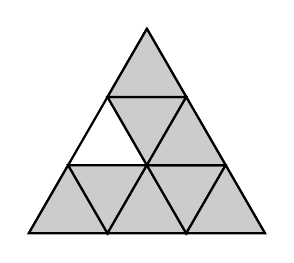
\begin{tikzpicture}
    \newcommand*\rows{3}
    \foreach \row in {0, 1, ...,\rows} {
    \draw[thick] ($\row*(0.5, {0.5*sqrt(3)})$) -- ($(\rows,0)+\row*(-0.5, {0.5*sqrt(3)})$);
    \draw[thick] ($\row*(1, 0)$) -- ($(\rows/2,{\rows/2*sqrt(3)})+\row*(0.5,{-0.5*sqrt(3)})$);
    \draw[thick] ($\row*(1, 0)$) -- ($(0,0)+\row*(0.5,{0.5*sqrt(3)})$);}
    %polyform
    \( \createtri{0}{0}{1}{0}{0.5}{0.866} \);
    \( \createtri{1}{0}{1.5}{0.866}{0.5}{0.866} \);
    \( \createtri{1}{0}{2}{0}{1.5}{0.866} \);
    \( \createtri{2}{0}{2.5}{0.866}{1.5}{0.866} \);
    \( \createtri{2}{0}{3}{0}{2.5}{0.866} \);
    \( \createtri{1.5}{0.866}{2}{1.732}{1}{1.732} \);
    \( \createtri{1.5}{0.866}{2.5}{0.866}{2}{1.732} \);
    \( \createtri{1}{1.732}{2}{1.732}{1.5}{2.598} \);
    \end{tikzpicture}%
  }
  & $\displaystyle \triangle^{T*}_n$  & $\displaystyle \sum_{k=0}^{n-1} \binom{2k}{k}$\\
  \resizebox{0.1\textwidth}{!}{%
  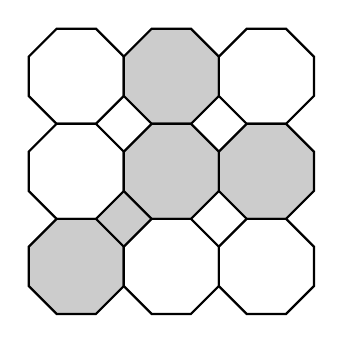
\begin{tikzpicture}
    %polyform
    \filldraw[gray!40](0.0,0.3535) -- (0.3535,0.0) -- 
            (0.8535,0.0) -- (1.207,0.3535) -- 
            (1.207,0.8535) -- (0.8535,1.207) -- 
            (0.3535,1.207) -- (0.0,0.8535) -- cycle;
    \filldraw[gray!40] (1.207,1.5605) -- (1.5605,1.207) -- 
            (2.0605,1.207) -- (2.414,1.5605) -- 
            (2.414,2.0605) -- (2.0605,2.414) -- 
            (1.5605,2.414) -- (1.207,2.0605) -- cycle;     
    \filldraw[gray!40] (1.207,2.7675) -- (1.5605,2.414) -- 
            (2.0605,2.414) -- (2.414,2.7675) -- 
            (2.414,3.2675) -- (2.0605,3.6210000000000004) -- 
            (1.5605,3.6210000000000004) -- (1.207,3.2675) -- cycle;
    \filldraw[gray!40] (2.414,1.5605) -- (2.7675,1.207) -- 
            (3.2675,1.207) -- (3.6210000000000004,1.5605) -- 
            (3.6210000000000004,2.0605) -- (3.2675,2.414) -- 
            (2.7675,2.414) -- (2.414,2.0605) -- cycle;
            
    \filldraw[gray!40] (1.207,0.8535) -- (0.8535,1.207) -- (1.207,1.5605) -- (1.5605,1.207) -- cycle;

    %lattice
    \draw[thick] (0.0,0.3535) -- (0.3535,0.0) -- 
        (0.8535,0.0) -- (1.207,0.3535) -- 
        (1.207,0.8535) -- (0.8535,1.207) -- 
        (0.3535,1.207) -- (0.0,0.8535) -- cycle;
    \draw[thick] (0.0,1.5605) -- (0.3535,1.207) -- 
        (0.8535,1.207) -- (1.207,1.5605) -- 
        (1.207,2.0605) -- (0.8535,2.414) -- 
        (0.3535,2.414) -- (0.0,2.0605) -- cycle;
    \draw[thick] (0.0,2.7675) -- (0.3535,2.414) -- 
        (0.8535,2.414) -- (1.207,2.7675) -- 
        (1.207,3.2675) -- (0.8535,3.6210000000000004) -- 
        (0.3535,3.6210000000000004) -- (0.0,3.2675) -- cycle;
        
        
    \draw[thick] (1.207,0.3535) -- (1.5605,0.0) -- 
        (2.0605,0.0) -- (2.414,0.3535) -- 
        (2.414,0.8535) -- (2.0605,1.207) -- 
        (1.5605,1.207) -- (1.207,0.8535) -- cycle;
    \draw[thick] (1.207,1.5605) -- (1.5605,1.207) -- 
        (2.0605,1.207) -- (2.414,1.5605) -- 
        (2.414,2.0605) -- (2.0605,2.414) -- 
        (1.5605,2.414) -- (1.207,2.0605) -- cycle;
    \draw[thick] (1.207,2.7675) -- (1.5605,2.414) -- 
        (2.0605,2.414) -- (2.414,2.7675) -- 
        (2.414,3.2675) -- (2.0605,3.6210000000000004) -- 
        (1.5605,3.6210000000000004) -- (1.207,3.2675) -- cycle;
        
        
    \draw[thick] (2.414,0.3535) -- (2.7675,0.0) -- 
        (3.2675,0.0) -- (3.6210000000000004,0.3535) -- 
        (3.6210000000000004,0.8535) -- (3.2675,1.207) -- 
        (2.7675,1.207) -- (2.414,0.8535) -- cycle;
    \draw[thick] (2.414,1.5605) -- (2.7675,1.207) -- 
        (3.2675,1.207) -- (3.6210000000000004,1.5605) -- 
        (3.6210000000000004,2.0605) -- (3.2675,2.414) -- 
        (2.7675,2.414) -- (2.414,2.0605) -- cycle;
    \draw[thick] (2.414,2.7675) -- (2.7675,2.414) -- 
        (3.2675,2.414) -- (3.6210000000000004,2.7675) -- 
        (3.6210000000000004,3.2675) -- (3.2675,3.6210000000000004) -- 
        (2.7675,3.6210000000000004) -- (2.414,3.2675) -- cycle;
    \end{tikzpicture}
  } 
  & $\displaystyle R^{\theta}_{w,\ell}$ & See Theorem \ref{thm:octagonal}\\
\end{tblr}
\end{center}

Each result includes visuals for both the traditional representation and the labelled dual representation. The empty set in the dual graph representation will be replaced with a black node for simplicity.

\subsection{Minimal Inscribed Polyforms in \texorpdfstring{$\mathbf{\triangle^{T}_n}$}{Tn}}

The first solved case we will examine is the triangular analogue to Theorem~\ref{thm:minimalsformula}. 

\begin{center}
    \begin{minipage}{0.25\textwidth}
        \centering
        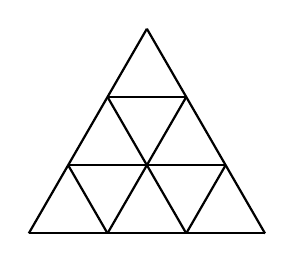
\begin{tikzpicture}
        \newcommand*\rows{3}
        \foreach \row in {0, 1, ...,\rows} {
            \draw[thick] ($\row*(0.5, {0.5*sqrt(3)})$) -- ($(\rows,0)+\row*(-0.5, {0.5*sqrt(3)})$);
            \draw[thick] ($\row*(1, 0)$) -- ($(\rows/2,{\rows/2*sqrt(3)})+\row*(0.5,{-0.5*sqrt(3)})$);
            \draw[thick] ($\row*(1, 0)$) -- ($(0,0)+\row*(0.5,{0.5*sqrt(3)})$);}
        \end{tikzpicture}
    \end{minipage}\hfill
    \begin{minipage}{0.25\textwidth}
        \centering
        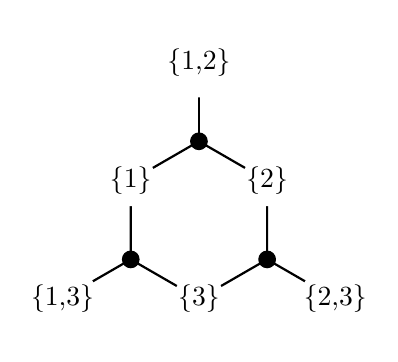
\begin{tikzpicture}
        %edges
        \draw[thick] (0,0) -- (0.866,0.5);
        \draw[thick] (3.464,0) -- (2.598,0.5);
        \draw[thick] (1.732,2) -- (1.732,3);
        \draw[thick] (0.866,0.5) -- (1.732,0) -- (2.598,0.5) -- (2.598,1.5) -- (1.732,2) -- (0.866,1.5) -- (0.866,0.5);
        %nodes
        \( \lablnode{0}{0}{1,3} \)
        \( \lablnode{1.732}{0}{3} \)
        \draw[fill=black] (0.866,0.5) circle (3pt);
        \( \lablnode{0.866}{1.5}{1} \)
        \draw[fill=black] (2.598,0.5) circle (3pt);
        \( \lablnode{3.464}{0}{2,3} \)
        \( \lablnode{2.598}{1.5}{2} \)
        \draw[fill=black] (1.732,2) circle (3pt);
        \( \lablnode{1.732}{3}{1,2} \)
        \end{tikzpicture}
    \end{minipage}\hfill
    \begin{minipage}{0.25\textwidth}
        \centering
        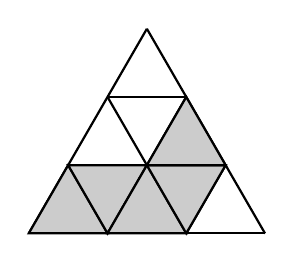
\begin{tikzpicture}
        \newcommand*\rows{3}
        \foreach \row in {0, 1, ...,\rows} {
            \draw[thick] ($\row*(0.5, {0.5*sqrt(3)})$) -- ($(\rows,0)+\row*(-0.5, {0.5*sqrt(3)})$);
            \draw[thick] ($\row*(1, 0)$) -- ($(\rows/2,{\rows/2*sqrt(3)})+\row*(0.5,{-0.5*sqrt(3)})$);
            \draw[thick] ($\row*(1, 0)$) -- ($(0,0)+\row*(0.5,{0.5*sqrt(3)})$);}
    %polyform
    \( \createtri{0}{0}{1}{0}{0.5}{0.866} \);
    \( \createtri{1}{0}{1.5}{0.866}{0.5}{0.866} \);
    \( \createtri{1}{0}{2}{0}{1.5}{0.866} \);
    \( \createtri{2}{0}{2.5}{0.866}{1.5}{0.866} \);
    \( \createtri{1.5}{0.866}{2.5}{0.866}{2}{1.732} \);

        \end{tikzpicture}
    \end{minipage}\hfill
    \captionof{figure}{The tiling and dual representation of $\triangle^{T}_3$ and an example polyform}
\end{center}

Let us call the family of triangles one can make $\triangle^{T}_n$, where $n$ designates the number of triangles touching a side, and the superscript $T$ designates that it is in a triangular lattice. Here $k=3$, and $m(\triangle^T_n) = 2n-1$. 

\begin{theorem}\label{thm: tri in tri}
The number of minimal inscribed polyforms $\rho(\triangle^T_n)$ for $n \geq 1$ is given by the following formula.

\begin{equation}\label{eq: triangle in triangle}
    \rho(\triangle^T_n) = ((n-1)^2 +2)2^{n-2}.
\end{equation}
\end{theorem}

\begin{proof}

Here we partition $\triangle^{T}_n$ into $3$ distinct subsets. Let us call the subset that contains the polyforms that contain $1$ or $2$ corner cells $S_1$. Then let us call the subset of polyforms not contained in $S_1$ that have cells with maximum degree of $2$ to be $S_2$. Finally let us call the subset of polyforms that have a maximum degree of $3$ to be $S_3$. We then write $\rho(\triangle^T_n) = |S_1| + |S_2| + |S_3|$.

\begin{center}
    \begin{minipage}{0.25\textwidth}
        \centering
        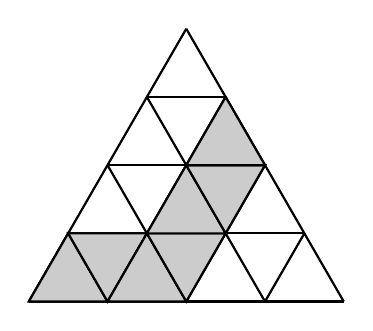
\begin{tikzpicture}
        \newcommand*\rows{4}
        \foreach \row in {0, 1, ...,\rows} {
            \draw[thick] ($\row*(0.5, {0.5*sqrt(3)})$) -- ($(\rows,0)+\row*(-0.5, {0.5*sqrt(3)})$);
            \draw[thick] ($\row*(1, 0)$) -- ($(\rows/2,{\rows/2*sqrt(3)})+\row*(0.5,{-0.5*sqrt(3)})$);
            \draw[thick] ($\row*(1, 0)$) -- ($(0,0)+\row*(0.5,{0.5*sqrt(3)})$);}
    %polyform
    \( \createtri{0}{0}{1}{0}{0.5}{0.866} \);
    \( \createtri{1}{0}{1.5}{0.866}{0.5}{0.866} \);
    \( \createtri{1}{0}{2}{0}{1.5}{0.866} \);
    \( \createtri{2}{0}{2.5}{0.866}{1.5}{0.866} \);
    \( \createtri{1.5}{0.866}{2.5}{0.866}{2}{1.732} \);
    \( \createtri{2.5}{0.866}{3}{1.732}{2}{1.732} \);
    \( \createtri{2.5}{2.598}{3}{1.732}{2}{1.732} \);
        \end{tikzpicture}
    \end{minipage}\hfill
    \begin{minipage}{0.25\textwidth}
        \centering
        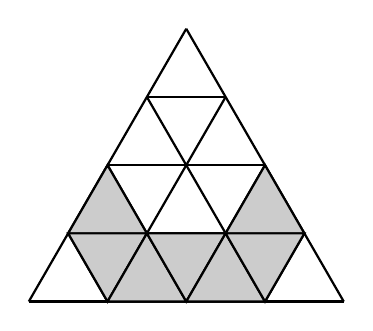
\begin{tikzpicture}
        \newcommand*\rows{4}
        \foreach \row in {0, 1, ...,\rows} {
            \draw[thick] ($\row*(0.5, {0.5*sqrt(3)})$) -- ($(\rows,0)+\row*(-0.5, {0.5*sqrt(3)})$);
            \draw[thick] ($\row*(1, 0)$) -- ($(\rows/2,{\rows/2*sqrt(3)})+\row*(0.5,{-0.5*sqrt(3)})$);
            \draw[thick] ($\row*(1, 0)$) -- ($(0,0)+\row*(0.5,{0.5*sqrt(3)})$);}
    %polyform
    \( \createtri{0.5}{0.866}{1.5}{0.866}{1}{1.732} \);
    \( \createtri{1}{0}{1.5}{0.866}{0.5}{0.866} \);
    \( \createtri{1}{0}{2}{0}{1.5}{0.866} \);
    \( \createtri{2}{0}{2.5}{0.866}{1.5}{0.866} \);
    \( \createtri{2.5}{0.866}{3.5}{0.866}{3}{1.732} \);
    \( \createtri{2}{0}{3}{0}{2.5}{0.866} \);
    \( \createtri{3}{0}{3.5}{0.866}{2.5}{0.866} \);
        \end{tikzpicture}
    \end{minipage}\hfill
    \begin{minipage}{0.25\textwidth}
        \centering
        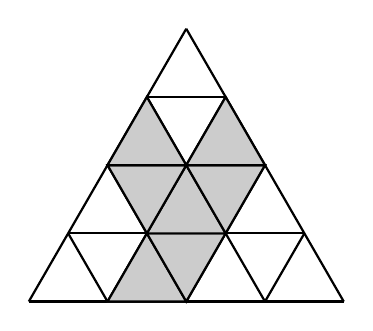
\begin{tikzpicture}
        \newcommand*\rows{4}
        \foreach \row in {0, 1, ...,\rows} {
            \draw[thick] ($\row*(0.5, {0.5*sqrt(3)})$) -- ($(\rows,0)+\row*(-0.5, {0.5*sqrt(3)})$);
            \draw[thick] ($\row*(1, 0)$) -- ($(\rows/2,{\rows/2*sqrt(3)})+\row*(0.5,{-0.5*sqrt(3)})$);
            \draw[thick] ($\row*(1, 0)$) -- ($(0,0)+\row*(0.5,{0.5*sqrt(3)})$);}
    %polyform

    \( \createtri{1}{0}{2}{0}{1.5}{0.866} \);
    \( \createtri{2}{0}{2.5}{0.866}{1.5}{0.866} \);
    \( \createtri{1.5}{0.866}{2.5}{0.866}{2}{1.732} \);
    \( \createtri{1.5}{0.866}{2}{1.732}{1}{1.732} \);
    \( \createtri{1.5}{2.598}{2}{1.732}{1}{1.732} \);
    \( \createtri{2.5}{0.866}{3}{1.732}{2}{1.732} \);
    \( \createtri{2.5}{2.598}{3}{1.732}{2}{1.732} \);

        \end{tikzpicture}
    \end{minipage}\hfill
    \captionof{figure}{Polyforms in $S_1$, $S_2$, and $S_3$}
\end{center}

\textbf{\textit{Case 1.}} Let $C(n)$ be the number of polyforms that contain the bottom left cell. The binomial theorem immediately gives that $C(n) = 2^{n-1}$. Applying this argument to each corner will double count the $3$ minimal polyominos that contain $2$ corners, and so $|S_1| = 3(2^{n-1} - 1)$.

\textbf{\textit{Case 2.}} All polyforms in $S_2$ are of the form 

\begin{center}
    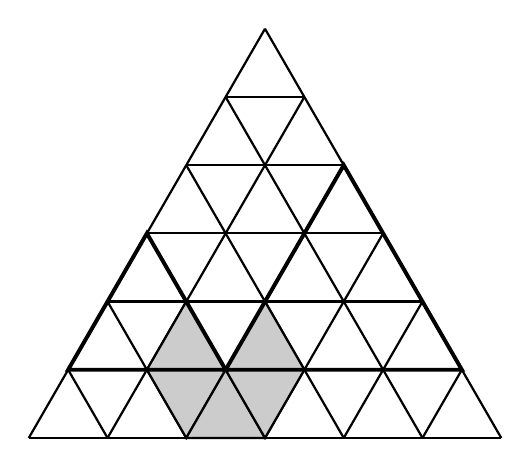
\begin{tikzpicture}
        \newcommand*\rows{6}
        \foreach \row in {0, 1, ...,\rows} {
        \draw[thick] ($\row*(0.5, {0.5*sqrt(3)})$) -- ($(\rows,0)+\row*(-0.5, {0.5*sqrt(3)})$);
        \draw[thick] ($\row*(1, 0)$) -- ($(\rows/2,{\rows/2*sqrt(3)})+\row*(0.5,{-0.5*sqrt(3)})$);
        \draw[thick] ($\row*(1, 0)$) -- ($(0,0)+\row*(0.5,{0.5*sqrt(3)})$);}
        %polyform
        \( \createtri{1.5}{0.866}{2.5}{0.866}{2}{1.732} \); %2.5,0.866
        \( \createtri{2}{0}{2.5}{0.866}{1.5}{0.866} \);
        \( \createtri{2.5}{0.866}{3.5}{0.866}{3}{1.732} \);
        \( \createtri{2}{0}{3}{0}{2.5}{0.866} \);
        \( \createtri{3}{0}{3.5}{0.866}{2.5}{0.866} \);

        \draw[line width=0.5mm] (0.5,0.866) -- (2.5,0.866) -- (1.5,2.598) --cycle;
        \draw[line width=0.5mm] (2.5,0.866) -- (5.5,0.866) -- (4,3.464) --cycle;
    \end{tikzpicture}
\end{center}

\noindent where the triangles in bold can be seen as smaller versions of case 1. Suppose we consider the polyforms with this ``U" shape on the bottom edge. If we index the cells that touch the bottom edge $1$ to $n$ from left to right, then there exist minimal inscribed polyforms that contain this ``U" shape on cells $2$ through $n-1$. These ``U" shapes can also be longer, shown below.

\begin{center}
    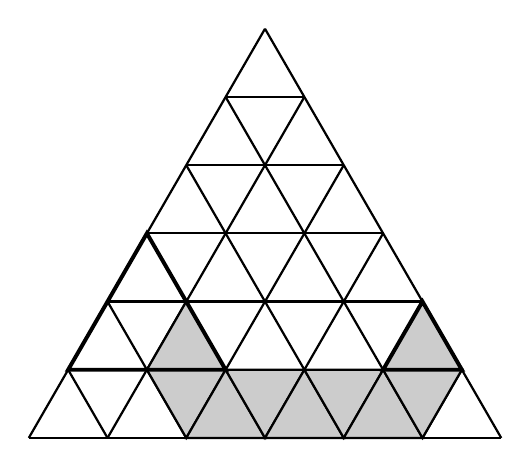
\begin{tikzpicture}
        \newcommand*\rows{6}
        \foreach \row in {0, 1, ...,\rows} {
        \draw[thick] ($\row*(0.5, {0.5*sqrt(3)})$) -- ($(\rows,0)+\row*(-0.5, {0.5*sqrt(3)})$);
        \draw[thick] ($\row*(1, 0)$) -- ($(\rows/2,{\rows/2*sqrt(3)})+\row*(0.5,{-0.5*sqrt(3)})$);
        \draw[thick] ($\row*(1, 0)$) -- ($(0,0)+\row*(0.5,{0.5*sqrt(3)})$);}
        %polyform
        \( \createtri{1.5}{0.866}{2.5}{0.866}{2}{1.732} \); %2.5,0.866
        \( \createtri{2}{0}{2.5}{0.866}{1.5}{0.866} \);
        
        \( \createtri{2}{0}{3}{0}{2.5}{0.866} \);
        \( \createtri{3}{0}{3.5}{0.866}{2.5}{0.866} \);
        \( \createtri{3}{0}{4}{0}{3.5}{0.866} \);
        \( \createtri{4}{0}{4.5}{0.866}{3.5}{0.866} \);
        \( \createtri{4}{0}{5}{0}{4.5}{0.866} \);
        \( \createtri{5}{0}{5.5}{0.866}{4.5}{0.866} \);

        \( \createtri{4.5}{0.866}{5.5}{0.866}{5}{1.732} \);

        \draw[line width=0.5mm] (0.5,0.866) -- (2.5,0.866) -- (1.5,2.598) --cycle;
        \draw[line width=0.5mm] (4.5,0.866) -- (5.5,0.866) -- (5,1.732) --cycle;
    \end{tikzpicture}
\end{center}

If we let $k$ represent the index of the left most edge cell that the ``U" shape contains, and $p$ the total number of edge cells the ``U" shape contains, we can write the following sum

$$E(n) = \sum_{k=2}^{n-1}\sum_{p=1}^{n-k}(2^{k-2})(2^{n-k-p}),$$

which after simplifying and applying the same argument for each edge, gives
$$|S_2| = 3E(n) = 3(n-3)2^{n-2}+3.$$

\textbf{\textit{Case 3.}}  All polyforms in $S_3$ are of the form

\begin{center}
    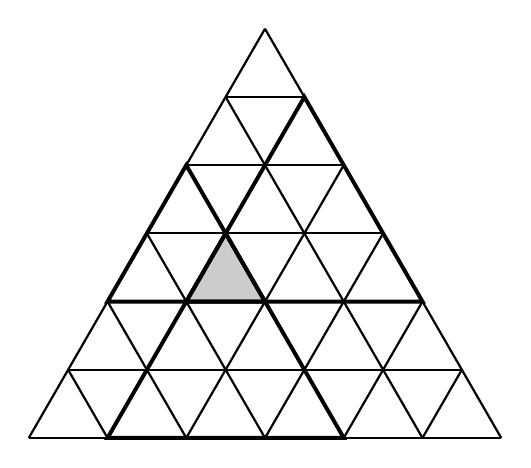
\begin{tikzpicture}
        \newcommand*\rows{6}
        \foreach \row in {0, 1, ...,\rows} {
        \draw[thick] ($\row*(0.5, {0.5*sqrt(3)})$) -- ($(\rows,0)+\row*(-0.5, {0.5*sqrt(3)})$);
        \draw[thick] ($\row*(1, 0)$) -- ($(\rows/2,{\rows/2*sqrt(3)})+\row*(0.5,{-0.5*sqrt(3)})$);
        \draw[thick] ($\row*(1, 0)$) -- ($(0,0)+\row*(0.5,{0.5*sqrt(3)})$);}
        %polyform
        \( \createtri{2}{1.732}{3}{1.732}{2.5}{2.598} \);

        \draw[line width=0.5mm] (3,1.732) -- (2,3.464) -- (1,1.732) --cycle;
        \draw[line width=0.5mm] (2.5,2.598) -- (1,0) -- (4,0) --cycle;
        \draw[line width=0.5mm] (2,1.732) -- (5,1.732) -- (3.5,4.33) --cycle;
    \end{tikzpicture}
\end{center}

\noindent again where the triangles in bold can be seen as smaller versions of case 1. This leads us to write the sum

$$|S_3| = \sum_{i=1}^{n-3}\sum_{j=1}^{i}(2^{j})(2^{n-i-2})(2^{i-j+1}) = (n-2)(n-3)2^{n-2},$$
\noindent where $i$ and $j$ count over the cells where the sides of the cell are parallel to the side of the larger triangle in the interior $(n-3)$-triangle. This gives $\rho(\triangle^T_n) = |S_1| + |S_2| + |S_3| =((n-1)^2 +2)2^{n-2}$.

\end{proof}

\noindent The first terms of $\rho(\triangle^T_n)$ for $n \geq 1$ are $1, 3, 12, 44, 144, 432, 1216, \dots$ (A356888 \cite{oeis}). The next solved family is similar. 

\subsection{Minimal Inscribed Polyforms in \texorpdfstring{$\mathbf{\triangle^{H}_n}$}{Hn} }

\begin{center}
    \begin{minipage}{0.25\textwidth}
        \centering
        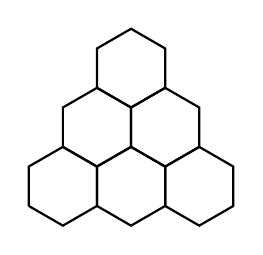
\begin{tikzpicture}
        %lattice
        \draw[thick] (0,0.25) -- (0.433,0) -- (0.866,0.25) -- (0.866,0.75) -- (0.433,1) -- (0,0.75) -- (0,0.25);
        \draw[thick] (0.866,0.25) -- (1.299,0) -- (1.732,0.25) -- (1.732,0.75) -- (1.299,1) -- (0.866,0.75) -- (0.866,0.25);
        \draw[thick] (1.732,0.25) -- (2.165,0) -- (2.598,0.25) -- (2.598,0.75) -- (2.165,1) -- (1.732,0.75) -- (1.732,0.25);
        
        \draw[thick] (0.433,1) -- (0.866,0.75) -- (1.299,1) -- (1.299,1.5) -- (0.866,1.75) -- (0.433,1.5) -- (0.433,1);
        \draw[thick] (1.299,1) -- (1.732,0.75) -- (2.165,1) -- (2.165,1.5) -- (1.732,1.75) -- (1.299,1.5) -- (1.299,1);
        
        \draw[thick] (0.866,1.75) -- (1.299,1.5) -- (1.732,1.75) -- (1.732,2.25) -- (1.299,2.5) -- (0.866,2.25) -- (0.866,1.75);
        \end{tikzpicture}
    \end{minipage}\hfill
    \begin{minipage}{0.25\textwidth}
        \centering
        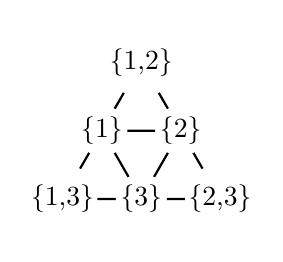
\begin{tikzpicture}
        %edges
        \draw[thick] (0,0) -- (1,0) -- (2,0) -- (1.5,0.866) -- (1,1.732) -- (0.5,0.866);
        \draw[thick] (0.5,0.866) -- (1.5, 0.866) -- (1,0) -- (0.5,0.866) -- (0,0);
        %nodes
        \( \lablnode{0}{0}{1,3} \)
        \( \lablnode{1}{0}{3} \)
        \( \lablnode{2}{0}{2,3} \)
        \( \lablnode{0.5}{0.866}{1} \)
        \( \lablnode{1.5}{0.866}{2} \)
        \( \lablnode{1}{1.732}{1,2} \)
        \end{tikzpicture}
    \end{minipage}\hfill
    \begin{minipage}{0.25\textwidth}
        \centering
        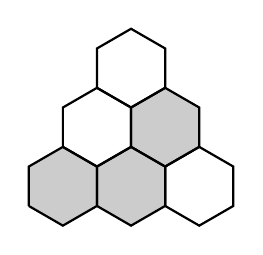
\begin{tikzpicture}
        %polyform
        %\filldraw[gray!40] (0,0.25) -- (0.433,0) -- (0.866,0.25) -- (0.866,0.75) -- (0.433,1) -- (0,0.75) -- (0,0.25);
        \filldraw[gray!40] (0,0.25) -- (0.433,0) -- (0.866,0.25) -- (1.299,0) -- (1.732,0.25) -- (1.732,0.75) -- (2.165,1) -- (2.165,1.5) -- (1.732,1.75) -- (1.299,1.5) -- (1.299,1) -- (0.866,0.75) -- (0.433,1) -- (0,0.75) -- (0,0.25);
        %\filldraw[gray!40] \draw[thick] (0.866,0.25) -- (1.299,0) -- (1.732,0.25) -- (1.732,0.75) -- (1.299,1) -- (0.866,0.75) -- (0.866,0.25);
        %\filldraw[gray!40] (1.299,1) -- (1.732,0.75) -- (2.165,1) -- (2.165,1.5) -- (1.732,1.75) -- (1.299,1.5) -- (1.299,1);
        %lattice
        \draw[thick] (0,0.25) -- (0.433,0) -- (0.866,0.25) -- (0.866,0.75) -- (0.433,1) -- (0,0.75) -- (0,0.25);
        \draw[thick] (0.866,0.25) -- (1.299,0) -- (1.732,0.25) -- (1.732,0.75) -- (1.299,1) -- (0.866,0.75) -- (0.866,0.25);
        \draw[thick] (1.732,0.25) -- (2.165,0) -- (2.598,0.25) -- (2.598,0.75) -- (2.165,1) -- (1.732,0.75) -- (1.732,0.25);
        
        \draw[thick] (0.433,1) -- (0.866,0.75) -- (1.299,1) -- (1.299,1.5) -- (0.866,1.75) -- (0.433,1.5) -- (0.433,1);
        \draw[thick] (1.299,1) -- (1.732,0.75) -- (2.165,1) -- (2.165,1.5) -- (1.732,1.75) -- (1.299,1.5) -- (1.299,1);
        
        \draw[thick] (0.866,1.75) -- (1.299,1.5) -- (1.732,1.75) -- (1.732,2.25) -- (1.299,2.5) -- (0.866,2.25) -- (0.866,1.75);
        \end{tikzpicture}
    \end{minipage}
    \captionof{figure}{The tiling and dual representation of $\triangle^H_3$ and an example polyform}
\end{center}

Let us call the family of triangles you can make in the hexagonal lattice $\triangle^H_n$, where $n$ designates the number of hexagons touching a triangular side, and the superscript $H$ designates that it is in a hexagonal lattice. Here $k=3$, and $m(\triangle^H_n) = n$.

\begin{theorem}\label{thm: tri in hex}
The number of minimal inscribed polyforms $\rho(\triangle^H_n)$ for $n\geq 1$ is given by the following formula.

\begin{equation}
    \rho(\triangle^H_n) = \left( \binom{n}{2}+2 \right) 2^{n-2}.
\end{equation}
\end{theorem}

\begin{proof}

We partition $\triangle^H_n$ in the same way as $\triangle^T_n$. $S_1$ and $S_2$ are enumerated the same way. However, the sum for $S_3$ given in the proof of Theorem \ref{thm: tri in tri} triple counts shapes of the form
\begin{center}
     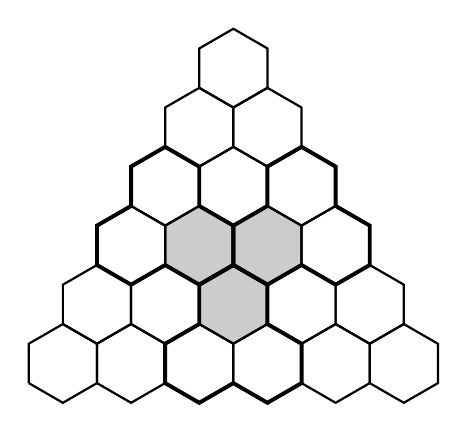
\begin{tikzpicture}
    %polyform
    \filldraw[gray!40] (2.165,1) -- (2.598,0.75) -- (3.031,1) -- (3.031,1.5) -- (2.598,1.75) -- (2.165,1.5) -- cycle;
    
    \filldraw[gray!40] (1.732,1.75) -- (2.165,1.5) -- (2.598,1.75) -- (2.598,2.25) -- (2.165,2.5) -- (1.732,2.25) -- (1.732,1.75);
    \filldraw[gray!40] (2.598,1.75) -- (3.031,1.5) -- (3.464,1.75) -- (3.464,2.25) -- (3.031,2.5) -- (2.598,2.25) -- cycle;
    

    %row 1
    \draw[thick] (0,0.25) -- (0.433,0) -- (0.866,0.25) -- (0.866,0.75) -- (0.433,1) -- (0,0.75) -- (0,0.25);
    \draw[thick] (0.866,0.25) -- (1.299,0) -- (1.732,0.25) -- (1.732,0.75) -- (1.299,1) -- (0.866,0.75) -- (0.866,0.25);
    \draw[thick] (1.732,0.25) -- (2.165,0) -- (2.598,0.25) -- (2.598,0.75) -- (2.165,1) -- (1.732,0.75) -- (1.732,0.25);
    \draw[thick] (2.598,0.25) -- (3.031,0) -- (3.464,0.25) -- (3.464,0.75) -- (3.031,1) -- (2.598,0.75) -- (2.598,0.25);
    \draw[thick] (3.464,0.25) -- (3.897,0) -- (4.33,0.25) -- (4.33,0.75) -- (3.897,1) -- (3.464,0.75) -- (3.464,0.25);
    \draw[thick] (4.33,0.25) -- (4.763,0) -- (5.196,0.25) -- (5.196,0.75) -- (4.763,1) -- (4.33,0.75) -- (4.33,0.25);
    
    %row 2
    \draw[thick] (0.433,1) -- (0.866,0.75) -- (1.299,1) -- (1.299,1.5) -- (0.866,1.75) -- (0.433,1.5) -- (0.433,1);
    \draw[thick] (1.299,1) -- (1.732,0.75) -- (2.165,1) -- (2.165,1.5) -- (1.732,1.75) -- (1.299,1.5) -- (1.299,1);
    \draw[thick] (2.165,1) -- (2.598,0.75) -- (3.031,1) -- (3.031,1.5) -- (2.598,1.75) -- (2.165,1.5) -- (2.165,1);
    \draw[thick] (3.031,1) -- (3.464,0.75) -- (3.897,1) -- (3.897,1.5) -- (3.464,1.75) -- (3.031,1.5) -- (3.031,1);
    \draw[thick] (3.897,1) -- (4.33,0.75) -- (4.763,1) -- (4.763,1.5) -- (4.33,1.75) -- (3.897,1.5) -- (3.897,1);
    
    %row 3
    \draw[thick] (0.866,1.75) -- (1.299,1.5) -- (1.732,1.75) -- (1.732,2.25) -- (1.299,2.5) -- (0.866,2.25) -- (0.866,1.75);
    \draw[thick] (1.732,1.75) -- (2.165,1.5) -- (2.598,1.75) -- (2.598,2.25) -- (2.165,2.5) -- (1.732,2.25) -- (1.732,1.75);
    \draw[thick] (2.598,1.75) -- (3.031,1.5) -- (3.464,1.75) -- (3.464,2.25) -- (3.031,2.5) -- (2.598,2.25) -- (2.598,1.75);
    \draw[thick] (3.464,1.75) -- (3.897,1.5) -- (4.33,1.75) -- (4.33,2.25) -- (3.897,2.5) -- (3.464,2.25) -- (3.464,1.75);
    
    %row 4
    \draw[thick] (1.299,2.5) -- (1.732,2.25) -- (2.165,2.5) -- (2.165,3) -- (1.732,3.25) -- (1.299,3) -- (1.299,2.5);
    \draw[thick] (2.165,2.5) -- (2.598,2.25) -- (3.031,2.5) -- (3.031,3) -- (2.598,3.25) -- (2.165,3) -- (2.165,2.5);
    \draw[thick] (3.031,2.5) -- (3.464,2.25) -- (3.897,2.5) -- (3.897,3) -- (3.464,3.25) -- (3.031,3) -- (3.031,2.5);
    
    %row 5
    \draw[thick] (1.732,3.25) -- (2.165,3) -- (2.598,3.25) -- (2.598,3.75) -- (2.165,4) -- (1.732,3.75) -- (1.732,3.25);
    \draw[thick] (2.598,3.25) -- (3.031,3) -- (3.464,3.25) -- (3.464,3.75) -- (3.031,4) -- (2.598,3.75) -- (2.598,3.25);

    %row 6
    \draw[thick] (2.165,4) -- (2.598,3.75) -- (3.031,4) -- (3.031,4.5) -- (2.598,4.75) -- (2.165,4.5) -- (2.165,4);

    %hilight
    \draw[line width = 0.5mm] (1.732,0.25) -- (2.165,0) -- (2.598,0.25) -- (2.598,0.25) -- (3.031,0) -- (3.464,0.25) -- (3.464,0.75) -- (3.031,1) -- (3.031,1) -- (3.031,1.5) -- (2.598,1.75) -- (2.165,1.5) -- (2.165,1) --(2.165,1) -- (1.732,0.75) -- (1.732,0.25);
    
    \draw[line width = 0.5mm] (2.598,1.75) -- (2.598,2.25) -- (2.165,2.5) -- (2.165,3) --(1.732,3.25) -- (1.299,3) -- (1.299,2.5) -- (0.866,2.25) -- (0.866,1.75) -- (1.299,1.5) --(1.732,1.75) -- (2.165,1.5) -- (2.598,1.75);
    \draw[line width = 0.5mm] (2.598,1.75) -- (3.031,1.5) -- (3.464,1.75) -- (3.897,1.5) -- (4.33,1.75) -- (4.33,2.25) -- (3.897,2.5) -- (3.897,3) -- (3.464,3.25) -- (3.031,3) -- (3.031,2.5) -- (3.031,2.5) -- (2.598,2.25) -- (2.598,1.75);
    
\end{tikzpicture}
\end{center}

\noindent where the bold triangles can be seen as smaller cases of $S_1$. The number of polyominos that are of this form are $(n-1)(n-2)2^{n-4}$. As these are triple counted by the sum for $S_3$, we get that
$$\rho(\triangle^H_n) = \rho(\triangle^T_n) - (n-1)(n-2)2^{n-3} = \left( \binom{n}{2}+2 \right) 2^{n-2}.$$

\end{proof}

The first terms in this sequence, for $n \geq 1$, are $1, 3, 10, 32, 96, 272, 736, \dots$ (A104270 \cite{oeis}).
%, with corresponding OGF $T(x) = \frac{x(1-3x+4x^2)}{(1-2x)^3}$.

\subsection{Minimal Inscribed Polyforms in \texorpdfstring{$\mathbf{\triangle^{R}_n}$}{Rn}}

\begin{center}
    \begin{minipage}{0.25\textwidth}
        \centering
        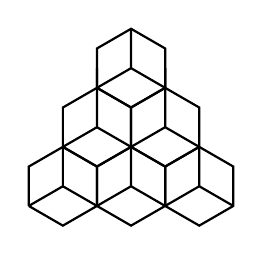
\begin{tikzpicture}
        %lattice
        \draw[thick] (0,0.25) -- (0.433,0) -- (0.866,0.25) -- (0.866,0.75) -- (0.433,1) -- (0,0.75) -- (0,0.25);
        \draw[thick] (0.866,0.25) -- (1.299,0) -- (1.732,0.25) -- (1.732,0.75) -- (1.299,1) -- (0.866,0.75) -- (0.866,0.25);
        \draw[thick] (1.732,0.25) -- (2.165,0) -- (2.598,0.25) -- (2.598,0.75) -- (2.165,1) -- (1.732,0.75) -- (1.732,0.25);
        
        \draw[thick] (0,0.25) -- (0.433,0.5) -- (0.433,1) -- (0.433,0.5) -- (0.866,0.25);
        \draw[thick] (0.866,0.25) -- (1.299,0.5) -- (1.299,1) -- (1.299,0.5) -- (1.732,0.25);
        \draw[thick] (1.732,0.25) -- (2.165,0.5) -- (2.165,1) -- (2.165,0.5) -- (2.598,0.25);
        
        
        \draw[thick] (0.433,1) -- (0.866,0.75) -- (1.299,1) -- (1.299,1.5) -- (0.866,1.75) -- (0.433,1.5) -- (0.433,1);
        \draw[thick] (1.299,1) -- (1.732,0.75) -- (2.165,1) -- (2.165,1.5) -- (1.732,1.75) -- (1.299,1.5) -- (1.299,1);
        
        \draw[thick] (0.433,1) -- (0.866,1.25) -- (0.866,2) -- (0.866,1.25) -- (1.299,1);
        \draw[thick] (1.299,1) -- (1.732,1.25) -- (1.732,2) -- (1.732,1.25) -- (2.165,1);
        
        
        \draw[thick] (0.866,1.75) -- (1.299,1.5) -- (1.732,1.75) -- (1.732,2.25) -- (1.299,2.5) -- (0.866,2.25) -- (0.866,1.75);
        
        \draw[thick] (0.866,1.75) -- (1.299,2) -- (1.299,2.5) -- (1.299,2) -- (1.732,1.75);
        \end{tikzpicture}
    \end{minipage}\hfill
    \begin{minipage}{0.25\textwidth}
        \centering
        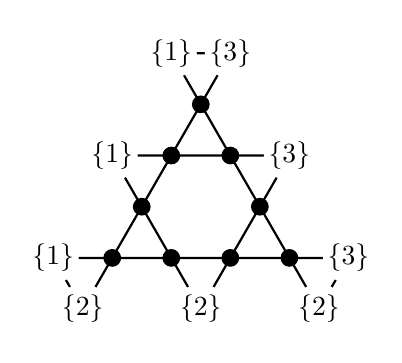
\begin{tikzpicture}
        %edges
        \draw[thick] (0,0.65) -- (0.75,0.65) -- (0.375,0) -- cycle;
        \draw[fill=black] (0.75,0.65) circle (3pt);
        \draw[thick] (0.75,0.65) -- (1.5,0.65) -- (1.125,1.3) -- cycle;
        \draw[fill=black] (1.5,0.65) circle (3pt);
        \draw[thick] (1.5,0.65) -- (2.25,0.65) -- (1.875,0) -- cycle;
        \draw[fill=black] (2.25,0.65) circle (3pt);
        \draw[thick] (2.25,0.65) -- (3,0.65) -- (2.625,1.3) -- cycle;
        \draw[fill=black] (3,0.65) circle (3pt);
        \draw[thick] (3,0.65) -- (3.75,0.65) -- (3.375,0) -- cycle;
        
        \draw[thick] (1.125,1.3) -- (0.75,1.95) -- (1.5,1.95) -- cycle;
        \draw[fill=black] (1.125,1.3) circle (3pt);
        \draw[thick] (2.625,1.3) -- (2.25,1.95) -- (3,1.95) -- cycle;
        \draw[fill=black] (2.625,1.3) circle (3pt);
        
        \draw[thick] (1.5,1.95) -- (2.25,1.95) -- (1.875,2.6) -- cycle;
        \draw[fill=black] (1.5,1.95) circle (3pt);
        \draw[fill=black] (2.25,1.95) circle (3pt);
        \draw[fill=black] (1.875,2.6) circle (3pt);
        
        \draw[thick] (1.5,3.25) -- (2.25,3.25) -- (1.875,2.6) -- cycle;
        
        %nodes
        \( \lablnode{0}{0.65}{1} \)
        \( \lablnode{0.375}{0}{2} \)
        \( \lablnode{1.875}{0}{2} \)
        \( \lablnode{3.375}{0}{2} \)
        \( \lablnode{3.75}{0.65}{3} \)
        \( \lablnode{0.75}{1.95}{1} \)
        \( \lablnode{3}{1.95}{3} \)
        \( \lablnode{1.5}{3.25}{1} \)
        \( \lablnode{2.25}{3.25}{3} \)
        
        \end{tikzpicture}
        
    \end{minipage}\hfill
    \begin{minipage}{0.25\textwidth}
        \centering
        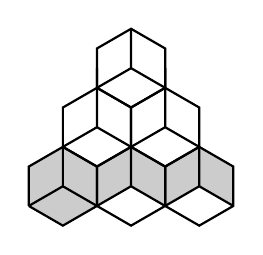
\begin{tikzpicture}
        %polyform
        \filldraw[gray!40] (0,0.25) -- (0.433,0) -- (0.866,0.25) -- (0.866,0.75) -- (0.433,1) -- (0,0.75) -- (0,0.25);
        \filldraw[gray!40] (0.866,0.25) -- (1.299,0.5) -- (1.299,1) -- (0.866,0.75) -- (0.866,0.25);
        \filldraw[gray!40] (1.732,0.25) -- (1.299,0.5) -- (1.299,1) -- (1.732,0.75) -- (1.732,0.25);
        \filldraw[gray!40] (1.732,0.25) -- (2.165,0.5) -- (2.165,1) -- (1.732,0.75) -- (1.732,0.25);
        \filldraw[gray!40] (2.598,0.25) -- (2.165,0.5) -- (2.165,1) -- (2.598,0.75) -- (2.598,0.25);
        
        %lattice
        \draw[thick] (0,0.25) -- (0.433,0) -- (0.866,0.25) -- (0.866,0.75) -- (0.433,1) -- (0,0.75) -- (0,0.25);
        \draw[thick] (0.866,0.25) -- (1.299,0) -- (1.732,0.25) -- (1.732,0.75) -- (1.299,1) -- (0.866,0.75) -- (0.866,0.25);
        \draw[thick] (1.732,0.25) -- (2.165,0) -- (2.598,0.25) -- (2.598,0.75) -- (2.165,1) -- (1.732,0.75) -- (1.732,0.25);
        
        
        \draw[thick] (0,0.25) -- (0.433,0.5) -- (0.433,1) -- (0.433,0.5) -- (0.866,0.25);
        \draw[thick] (0.866,0.25) -- (1.299,0.5) -- (1.299,1) -- (1.299,0.5) -- (1.732,0.25);
        \draw[thick] (1.732,0.25) -- (2.165,0.5) -- (2.165,1) -- (2.165,0.5) -- (2.598,0.25);
        
        
        \draw[thick] (0.433,1) -- (0.866,0.75) -- (1.299,1) -- (1.299,1.5) -- (0.866,1.75) -- (0.433,1.5) -- (0.433,1);
        \draw[thick] (1.299,1) -- (1.732,0.75) -- (2.165,1) -- (2.165,1.5) -- (1.732,1.75) -- (1.299,1.5) -- (1.299,1);
        
        \draw[thick] (0.433,1) -- (0.866,1.25) -- (0.866,2) -- (0.866,1.25) -- (1.299,1);
        \draw[thick] (1.299,1) -- (1.732,1.25) -- (1.732,2) -- (1.732,1.25) -- (2.165,1);
        
        
        \draw[thick] (0.866,1.75) -- (1.299,1.5) -- (1.732,1.75) -- (1.732,2.25) -- (1.299,2.5) -- (0.866,2.25) -- (0.866,1.75);
        
        \draw[thick] (0.866,1.75) -- (1.299,2) -- (1.299,2.5) -- (1.299,2) -- (1.732,1.75);
        \end{tikzpicture}
    \end{minipage}
    \captionof{figure}{The tiling and dual representation of $\triangle^R_3$ and an example polyform}\label{fig:tri in rhomb}
\end{center}

Let us call the family of triangles one can make $\triangle^R_n$, where $n$ designates the number of rhombuses touching a side, and the superscript $R$ designates that it is in a rhombic lattice. Here $k=3$, and $m(\triangle^R_n) = 2n+1$. 

\begin{theorem}
The number of minimal inscribed polyforms $\rho(\triangle^R_n)$ for $n \geq 1$ is given by the following formula.

\begin{equation}
    \rho(\triangle^R_n) = n(n+1)2^{n-2}.
\end{equation}
\end{theorem}

\begin{proof}

We partition $\triangle^R_n$ into two subsets. Let $S_1$ be the polyforms that contain the three corner most cells, and let $S_2 = S_1^c$. 

\begin{center}
    \begin{minipage}{0.45\textwidth}
    \centering
        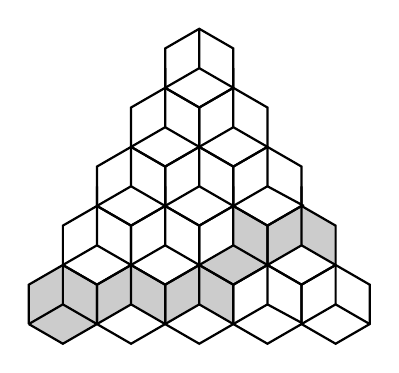
\begin{tikzpicture}
    %polyform
    \filldraw[gray!40] (0,0.25) -- (0.433,0) -- (0.866,0.25) -- (0.866,0.75) -- (0.433,1) -- (0,0.75) -- (0,0.25);
    \filldraw[gray!40] (0.866,0.25) -- (1.299,0.5) -- (1.299,1) -- (0.866,0.75) -- (0.866,0.25);
    \filldraw[gray!40] (1.732,0.25) -- (1.299,0.5) -- (1.299,1) -- (1.732,0.75) -- (1.732,0.25);
    \filldraw[gray!40] (1.732,0.25) -- (2.165,0.5) -- (2.165,1) -- (1.732,0.75) -- (1.732,0.25);
    \filldraw[gray!40] (2.598,0.25) -- (2.165,0.5) -- (2.165,1) -- (2.598,0.75) -- (2.598,0.25);
    \filldraw[gray!40] (2.165,1) -- (2.598,0.75) -- (3.031,1) -- (2.598,1.25) -- (2.165,1);
    \filldraw[gray!40] (3.031,1) -- (2.598,1.25) --(2.598,1.75) -- (3.031,1.5) -- (3.031,1);
    \filldraw[gray!40] (3.031,1) -- (3.031,1.5) -- (3.464,1.75) -- (3.464,1.25) -- (3.031,1);
    \filldraw[gray!40] (3.464,1.75) -- (3.464,1.25) -- (3.897,1) -- (3.897,1.5) -- (3.464,1.75);
        
    %row 1
    \draw[thick] (0,0.25) -- (0.433,0) -- (0.866,0.25) -- (0.866,0.75) -- (0.433,1) -- (0,0.75) -- (0,0.25);
    \draw[thick] (0.866,0.25) -- (1.299,0) -- (1.732,0.25) -- (1.732,0.75) -- (1.299,1) -- (0.866,0.75) -- (0.866,0.25);
    \draw[thick] (1.732,0.25) -- (2.165,0) -- (2.598,0.25) -- (2.598,0.75) -- (2.165,1) -- (1.732,0.75) -- (1.732,0.25);
    
    \draw[thick] (2.598,0.25) -- (3.031,0) -- (3.464,0.25) -- (3.464,0.75) -- (3.031,1) -- (2.598,0.75) -- (2.598,0.25);
    \draw[thick] (3.464,0.25) -- (3.897,0) -- (4.33,0.25) -- (4.33,0.75) -- (3.897,1) -- (3.464,0.75) -- (3.464,0.25);
    
    \draw[thick] (0,0.25) -- (0.433,0.5) -- (0.433,1) -- (0.433,0.5) -- (0.866,0.25);
    \draw[thick] (0.866,0.25) -- (1.299,0.5) -- (1.299,1) -- (1.299,0.5) -- (1.732,0.25);
    \draw[thick] (1.732,0.25) -- (2.165,0.5) -- (2.165,1) -- (2.165,0.5) -- (2.598,0.25);
    \draw[thick] (2.598,0.25) -- (3.031,0.5) -- (3.031,1) -- (3.031,0.5) -- (3.494,0.25);
    \draw[thick] (3.464,0.25) -- (3.897,0.5) -- (3.897,1) -- (3.897,0.5) -- (4.33,0.25);
    
    %row 2
    \draw[thick] (0.433,1) -- (0.866,0.75) -- (1.299,1) -- (1.299,1.5) -- (0.866,1.75) -- (0.433,1.5) -- (0.433,1);
    \draw[thick] (1.299,1) -- (1.732,0.75) -- (2.165,1) -- (2.165,1.5) -- (1.732,1.75) -- (1.299,1.5) -- (1.299,1);
    \draw[thick] (2.165,1) -- (2.598,0.75) -- (3.031,1) -- (3.031,1.5) -- (2.598,1.75) -- (2.165,1.5) -- (2.165,1);
    \draw[thick] (3.031,1) -- (3.464,0.75) -- (3.897,1) -- (3.897,1.5) -- (3.464,1.75) -- (3.031,1.5) -- (3.031,1);
    
    \draw[thick] (0.433,1) -- (0.866,1.25) -- (0.866,2) -- (0.866,1.25) -- (1.299,1);
    \draw[thick] (1.299,1) -- (1.732,1.25) -- (1.732,2) -- (1.732,1.25) -- (2.165,1);
    \draw[thick] (2.165,1) -- (2.598,1.25) -- (2.598,2) -- (2.598,1.25) -- (3.031,1);
    \draw[thick] (3.031,1) -- (3.464,1.25) -- (3.464,2) -- (3.464,1.25) -- (3.897,1);
    
    
    %row 3
    \draw[thick] (0.866,1.75) -- (1.299,1.5) -- (1.732,1.75) -- (1.732,2.25) -- (1.299,2.5) -- (0.866,2.25) -- (0.866,1.75);
    \draw[thick] (1.732,1.75) -- (2.165,1.5) -- (2.598,1.75) -- (2.598,2.25) -- (2.165,2.5) -- (1.732,2.25) -- (1.732,1.75);
    \draw[thick] (2.598,1.75) -- (3.031,1.5) -- (3.464,1.75) -- (3.464,2.25) -- (3.031,2.5) -- (2.598,2.25) -- (2.598,1.75);
    
    \draw[thick] (0.866,1.75) -- (1.299,2) -- (1.299,2.5) -- (1.299,2) -- (1.732,1.75);
    \draw[thick] (1.732,1.75) -- (2.165,2) -- (2.165,2.5) -- (2.165,2) -- (2.598,1.75);
    \draw[thick] (2.598,1.75) -- (3.031,2) -- (3.031,2.5) -- (3.031,2) -- (3.494,1.75);
    
    %row 4
    \draw[thick] (1.299,2.5) -- (1.732,2.25) -- (2.165,2.5) -- (2.165,3) -- (1.732,3.25) -- (1.299,3) -- (1.299,2.5);
    \draw[thick] (2.165,2.5) -- (2.598,2.25) -- (3.031,2.5) -- (3.031,3) -- (2.598,3.25) -- (2.165,3) -- (2.165,2.5);
    
    \draw[thick] (1.299,2.5) -- (1.732,2.75) -- (1.732,3.5) -- (1.732,2.75) -- (2.165,2.5);
    \draw[thick] (2.165,2.5) -- (2.598,2.75) -- (2.598,3.5) -- (2.598,2.75) -- (3.031,2.5);
    
    %row 5
    \draw[thick] (1.732,3.25) -- (2.165,3) -- (2.598,3.25) -- (2.598,3.75) -- (2.165,4) -- (1.732,3.75) -- (1.732,3.25);
    
    \draw[thick] (1.732,3.25) -- (2.165,3.5) -- (2.165,4) -- (2.165,3.5) -- (2.598,3.25);
    
\end{tikzpicture}
    \end{minipage}\hfill
    \begin{minipage}{0.45\textwidth}
    \centering
        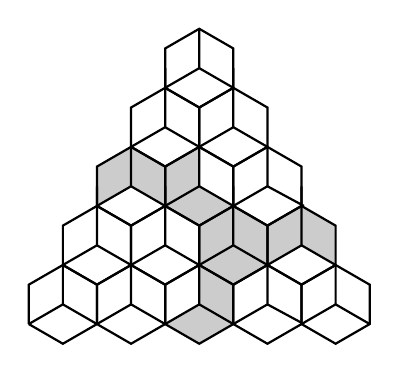
\begin{tikzpicture}
        %polyform
        \filldraw[gray!40] (0.866,1.75) -- (1.299,2) -- (1.299,2.5) -- (0.866,2.25) -- (0.866,1.75);
        \filldraw[gray!40] (1.732,1.75) -- (1.299,2) -- (1.299,2.5) -- (1.732,2.25) -- (1.732,1.75);
        \filldraw[gray!40] (1.732,1.75) -- (2.165,2) -- (2.165,2.5) -- (1.732,2.25) -- (1.732,1.75);
        \filldraw[gray!40] (1.732,1.75) -- (2.165,2) -- (2.598,1.75) -- (2.165,1.5) -- (1.732,1.75);

        
        \filldraw[gray!40] (1.732,0.25) -- (2.165,0) -- (2.598,0.25) -- (2.165,0.5) -- (1.732,0.25);
        \filldraw[gray!40] (2.165,1) -- (2.165,1.5) -- (2.598,1.75) -- (2.598,1.25) -- (2.165,1);
        \filldraw[gray!40] (2.598,0.25) -- (2.165,0.5) -- (2.165,1) -- (2.598,0.75) -- (2.598,0.25);

        
        \filldraw[gray!40] (2.165,1) -- (2.598,0.75) -- (3.031,1) -- (2.598,1.25) -- (2.165,1);
        \filldraw[gray!40] (3.031,1) -- (2.598,1.25) --(2.598,1.75) -- (3.031,1.5) -- (3.031,1);
        \filldraw[gray!40] (3.031,1) -- (3.031,1.5) -- (3.464,1.75) -- (3.464,1.25) -- (3.031,1);
        \filldraw[gray!40] (3.464,1.75) -- (3.464,1.25) -- (3.897,1) -- (3.897,1.5) -- (3.464,1.75);
        
    %row 1
    \draw[thick] (0,0.25) -- (0.433,0) -- (0.866,0.25) -- (0.866,0.75) -- (0.433,1) -- (0,0.75) -- (0,0.25);
    \draw[thick] (0.866,0.25) -- (1.299,0) -- (1.732,0.25) -- (1.732,0.75) -- (1.299,1) -- (0.866,0.75) -- (0.866,0.25);
    \draw[thick] (1.732,0.25) -- (2.165,0) -- (2.598,0.25) -- (2.598,0.75) -- (2.165,1) -- (1.732,0.75) -- (1.732,0.25);
    \draw[thick] (2.598,0.25) -- (3.031,0) -- (3.464,0.25) -- (3.464,0.75) -- (3.031,1) -- (2.598,0.75) -- (2.598,0.25);
    \draw[thick] (3.464,0.25) -- (3.897,0) -- (4.33,0.25) -- (4.33,0.75) -- (3.897,1) -- (3.464,0.75) -- (3.464,0.25);
    
    \draw[thick] (0,0.25) -- (0.433,0.5) -- (0.433,1) -- (0.433,0.5) -- (0.866,0.25);
    \draw[thick] (0.866,0.25) -- (1.299,0.5) -- (1.299,1) -- (1.299,0.5) -- (1.732,0.25);
    \draw[thick] (1.732,0.25) -- (2.165,0.5) -- (2.165,1) -- (2.165,0.5) -- (2.598,0.25);
    \draw[thick] (2.598,0.25) -- (3.031,0.5) -- (3.031,1) -- (3.031,0.5) -- (3.494,0.25);
    \draw[thick] (3.464,0.25) -- (3.897,0.5) -- (3.897,1) -- (3.897,0.5) -- (4.33,0.25);
    
    %row 2
    \draw[thick] (0.433,1) -- (0.866,0.75) -- (1.299,1) -- (1.299,1.5) -- (0.866,1.75) -- (0.433,1.5) -- (0.433,1);
    \draw[thick] (1.299,1) -- (1.732,0.75) -- (2.165,1) -- (2.165,1.5) -- (1.732,1.75) -- (1.299,1.5) -- (1.299,1);
    \draw[thick] (2.165,1) -- (2.598,0.75) -- (3.031,1) -- (3.031,1.5) -- (2.598,1.75) -- (2.165,1.5) -- (2.165,1);
    \draw[thick] (3.031,1) -- (3.464,0.75) -- (3.897,1) -- (3.897,1.5) -- (3.464,1.75) -- (3.031,1.5) -- (3.031,1);
    
    \draw[thick] (0.433,1) -- (0.866,1.25) -- (0.866,2) -- (0.866,1.25) -- (1.299,1);
    \draw[thick] (1.299,1) -- (1.732,1.25) -- (1.732,2) -- (1.732,1.25) -- (2.165,1);
    \draw[thick] (2.165,1) -- (2.598,1.25) -- (2.598,2) -- (2.598,1.25) -- (3.031,1);
    \draw[thick] (3.031,1) -- (3.464,1.25) -- (3.464,2) -- (3.464,1.25) -- (3.897,1);
    
    
    %row 3
    \draw[thick] (0.866,1.75) -- (1.299,1.5) -- (1.732,1.75) -- (1.732,2.25) -- (1.299,2.5) -- (0.866,2.25) -- (0.866,1.75);
    \draw[thick] (1.732,1.75) -- (2.165,1.5) -- (2.598,1.75) -- (2.598,2.25) -- (2.165,2.5) -- (1.732,2.25) -- (1.732,1.75);
    \draw[thick] (2.598,1.75) -- (3.031,1.5) -- (3.464,1.75) -- (3.464,2.25) -- (3.031,2.5) -- (2.598,2.25) -- (2.598,1.75);
    
    \draw[thick] (0.866,1.75) -- (1.299,2) -- (1.299,2.5) -- (1.299,2) -- (1.732,1.75);
    \draw[thick] (1.732,1.75) -- (2.165,2) -- (2.165,2.5) -- (2.165,2) -- (2.598,1.75);
    \draw[thick] (2.598,1.75) -- (3.031,2) -- (3.031,2.5) -- (3.031,2) -- (3.494,1.75);
    
    %row 4
    \draw[thick] (1.299,2.5) -- (1.732,2.25) -- (2.165,2.5) -- (2.165,3) -- (1.732,3.25) -- (1.299,3) -- (1.299,2.5);
    \draw[thick] (2.165,2.5) -- (2.598,2.25) -- (3.031,2.5) -- (3.031,3) -- (2.598,3.25) -- (2.165,3) -- (2.165,2.5);
    
    \draw[thick] (1.299,2.5) -- (1.732,2.75) -- (1.732,3.5) -- (1.732,2.75) -- (2.165,2.5);
    \draw[thick] (2.165,2.5) -- (2.598,2.75) -- (2.598,3.5) -- (2.598,2.75) -- (3.031,2.5);
    
    %row 5
    \draw[thick] (1.732,3.25) -- (2.165,3) -- (2.598,3.25) -- (2.598,3.75) -- (2.165,4) -- (1.732,3.75) -- (1.732,3.25);
    
    \draw[thick] (1.732,3.25) -- (2.165,3.5) -- (2.165,4) -- (2.165,3.5) -- (2.598,3.25);
    
\end{tikzpicture}
    \end{minipage}
    \captionof{figure}{Examples of Polyforms in $S_1$ and $S_2$ for $\rho(\triangle^R_5)$}
\end{center}

Similarly to Theorems \ref{thm: tri in tri} and Theorem \ref{thm: tri in hex}, $S_1$ can easily be enumerated using the binomial theorem to get $|S_1| = 2^{n-1}$. Also similarly, enumerating $S_2$ can be seen as the product of smaller cases of $S_1$. So each  of the $\frac{n(n+1)}{2}$ locations where the following three cells 

\begin{center}
    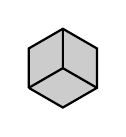
\begin{tikzpicture}
    \filldraw[gray!40] (0,0.25) -- (0.433,0) -- (0.866,0.25) -- (0.866,0.75) -- (0.433,1) -- (0,0.75) -- (0,0.25);

    \draw[thick] (0,0.25) -- (0.433,0) -- (0.866,0.25) -- (0.866,0.75) -- (0.433,1) -- (0,0.75) -- (0,0.25);
    \draw[thick] (0,0.25) -- (0.433,0.5) -- (0.433,1) -- (0.433,0.5) -- (0.866,0.25);
    \end{tikzpicture}
\end{center}

\noindent can be found has $2^{n-1}$ polyforms, which gives $\rho(\triangle^R_n) = n(n+1)2^{n-2}$.

\end{proof}

The first terms of this sequence, for $n \geq 1$, are $1, 6, 24, 80, 240, 672, 1792, \dots$ (A001788 \cite{oeis}).

\subsection{Minimal Inscribed Polyforms in \texorpdfstring{$\mathbf{\triangle^{K}_n}$}{Kn}}

\begin{center}
    \begin{minipage}{0.25\textwidth}
        \centering
        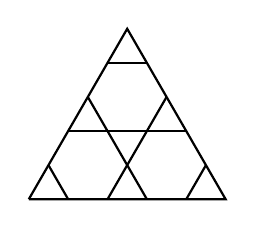
\begin{tikzpicture}
        %lattice
        \draw[thick] (0,0) -- (2.5,0) -- (1.25, 2.165) -- (0,0);
        \draw[thick] (1,1.732) -- (1.5,1.732);
        \draw[thick] (0.5,0) -- (0.25,0.433);
        \draw[thick] (2,0) -- (2.25,0.433);
        \draw[thick] (1,0) -- (1.75,1.299);
        \draw[thick] (1.5,0) -- (0.75,1.299);
        \draw[thick] (0.5,0.866) -- (2,0.866);
        \end{tikzpicture}
    \end{minipage}\hfill
    \begin{minipage}{0.25\textwidth}
        \centering
        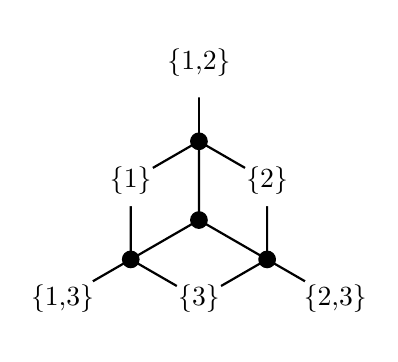
\begin{tikzpicture}
        %edges
        \draw[thick] (0,0) -- (0.866,0.5);
        \draw[thick] (3.464,0) -- (2.598,0.5);
        \draw[thick] (1.732,2) -- (1.732,3);
        \draw[thick] (0.866,0.5) -- (1.732,0) -- (2.598,0.5) -- (2.598,1.5) -- (1.732,2) -- (0.866,1.5) -- (0.866,0.5);
        \draw[thick] (0.866,0.5) -- (1.732,1) -- (1.732,2);
        \draw[thick] (1.732,1) -- (2.598,0.5);
        
        %nodes
        \( \lablnode{0}{0}{1,3} \)
        \( \lablnode{1.732}{0}{3} \)
        \draw[fill=black] (0.866,0.5) circle (3pt);
        \( \lablnode{0.866}{1.5}{1} \)
        \draw[fill=black] (2.598,0.5) circle (3pt);
        \( \lablnode{3.464}{0}{2,3} \)
        \( \lablnode{2.598}{1.5}{2} \)
        \draw[fill=black] (1.732,2) circle (3pt);
        \( \lablnode{1.732}{3}{1,2} \)
        \draw[fill=black] (1.732,1) circle (3pt);
        
        \end{tikzpicture}
    \end{minipage}\hfill
    \begin{minipage}{0.25\textwidth}
        \centering
        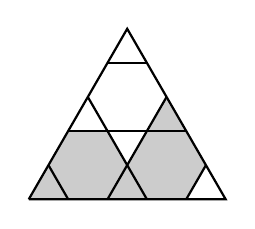
\begin{tikzpicture}
        %polyform
        \filldraw[gray!40] (0,0) -- (0.5,0) -- (0.25,0.433) -- cycle;
        \filldraw[gray!40] (1,0) -- (1.5,0) -- (1.25,0.433) -- cycle;
        \filldraw[gray!40] (1.5,0.866) -- (2,0.866) -- (1.75,1.299) -- cycle;
        
        \filldraw[gray!40] (0.25,0.433) -- (0.5,0) -- (1,0) -- (1.25, 0.433) -- (1,0.866) -- (0.5,0.866) -- (0.25,0.433);
        \filldraw[gray!40] (1.25,0.433) -- (1.5,0) -- (2,0) -- (2.25, 0.433) -- (2,0.866) -- (1.5,0.866) -- (1.25,0.433);
        
        %lattice
        \draw[thick] (0,0) -- (2.5,0) -- (1.25, 2.165) -- (0,0);
        \draw[thick] (1,1.732) -- (1.5,1.732);
        \draw[thick] (0.5,0) -- (0.25,0.433);
        \draw[thick] (2,0) -- (2.25,0.433);
        \draw[thick] (1,0) -- (1.75,1.299);
        \draw[thick] (1.5,0) -- (0.75,1.299);
        \draw[thick] (0.5,0.866) -- (2,0.866);
        \end{tikzpicture}
    \end{minipage}
    \captionof{figure}{The tiling and dual representation of $\triangle^K_n$ and an example polyform}
    \label{fig: bowtie lattice n is 3}
\end{center}

Let us call the family of triangles one can make $\triangle^K_n$, where $n$ designates the number of triangles touching a side, and the superscript $K$ designates that it is the hexagonal and triangular lattice shown above, which is often called a \textit{kagome} lattice. 

Again $k=3$, and $m(\triangle^K_n) = 2n-1$. 

\begin{theorem}\label{thm:tri in tri hex}
The number of minimal inscribed polyforms $\rho(\triangle^K_n)$ for $n \geq 2$ is given by the following formula.

\begin{equation}
    \rho(\triangle^K_n) = \left( n^2 + 3n +\frac{10}{3} \right) 4^{n-3} - \frac{1}{3}.
\end{equation}
\end{theorem}

\begin{proof}

We again partition $\triangle^K_n$ into $S_1$, $S_2$, and $S_3$. This proof is closely related to the proof of Theorem \ref{thm: tri in tri}, as we choose analogous definitions for $S_1$, $S_2$, and $S_3$.

\begin{center}
\begin{minipage}{0.25\textwidth}
    \centering
    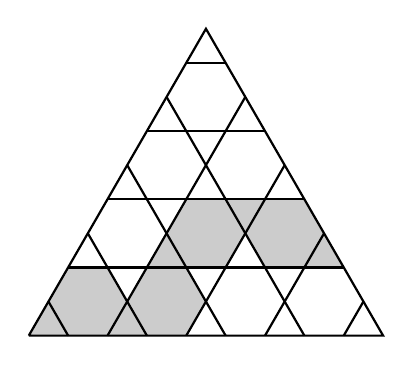
\begin{tikzpicture}
    %polyform
    \filldraw[gray!40] (0,0) -- (0.5,0) -- (0.25,0.433) -- cycle;
    \filldraw[gray!40] (0.5,0) -- (1,0) -- (1.25,0.433) -- (1,0.866) -- (0.5,0.866) -- (0.25,0.433) -- cycle;
    \filldraw[gray!40] (1,0) -- (1.5,0) -- (1.25,0.433) -- cycle;
    \filldraw[gray!40] (1.5,0) -- (2,0) -- (2.25,0.433) -- (2,0.866) -- (1.5,0.866) -- (1.25,0.433) -- cycle;
    \filldraw[gray!40] (1.5,0.866) -- (2,0.866) -- (1.75,1.299) -- cycle;
    \filldraw[gray!40] (2,0.866) -- (2.5,0.866) --  (2.75,1.299) -- (2.5,1.732) -- (2,1.732) -- (1.75,1.299) -- cycle;
    \filldraw[gray!40] (2.75,1.299) -- (2.5,1.732) -- (3.25,1.732);
    \filldraw[gray!40] (3,0.866) -- (3.5,0.866) --  (3.75,1.299) -- (3.5,1.732) -- (3,1.732) -- (2.75,1.299) -- cycle;
    \filldraw[gray!40] (3.5,0.866) -- (4,0.866) -- (3.75,1.299) -- cycle;
    
    %lattice
    \draw[thick] (0,0) -- (4.5,0) -- (2.25, 3.897) -- (0,0);
    \draw[thick] (1,0) -- (2.75,3.031);
    \draw[thick] (2,0) -- (3.25,2.165);
    \draw[thick] (3,0) -- (3.75,1.299);
    \draw[thick] (4,0) -- (4.25,0.433);
    
    \draw[thick] (3.5,0) -- (1.75,3.031);
    \draw[thick] (2.5,0) -- (1.25,2.165);
    \draw[thick] (1.5,0) -- (0.75,1.299);
    \draw[thick] (0.5,0) -- (0.25,0.433);
    
    \draw[thick] (0.5,0.866) -- (4,0.866);
    \draw[thick] (1,1.732) -- (3.5,1.732);
    \draw[thick] (1.5,2.598) -- (3,2.598);
    \draw[thick] (2,3.464) -- (2.5,3.464);
        
    \end{tikzpicture}
    %\captionof{figure}{A triangle in the hexagonal/triangular lattice}
    %\label{fig: triangle in hex/tri lattice}
\end{minipage}\hfill
\begin{minipage}{0.25\textwidth}
    \centering
    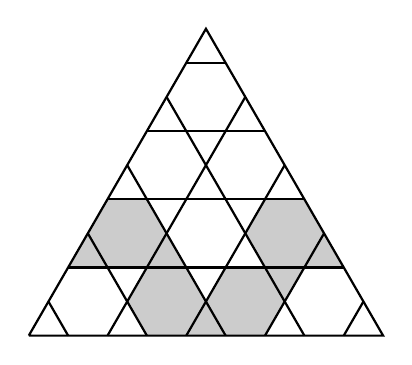
\begin{tikzpicture}
    %polyform
    \filldraw[gray!40] (1.5,0) -- (2,0) -- (2.25,0.433) -- (2,0.866) -- (1.5,0.866) -- (1.25,0.433) -- cycle;
    \filldraw[gray!40] (2,0) -- (2.5,0) -- (2.25,0.433) -- cycle;
    \filldraw[gray!40] (2.5,0) -- (3,0) -- (3.25,0.433) -- (3,0.866) -- (2.5,0.866) -- (2.25,0.433) -- cycle;
    \filldraw[gray!40] (1.5,0.866) -- (2,0.866) -- (1.75,1.299) -- cycle;
    \filldraw[gray!40] (1,0.866) -- (1.5,0.866) -- (1.75,1.299) -- (1.5,1.732) -- (1,1.732) -- (0.75,1.299) -- cycle;
    \filldraw[gray!40] (0.5,0.866) -- (1,0.866) -- (0.75,1.299) -- cycle;
    \filldraw[gray!40] (3.25,0.433) -- (3,0.866) -- (3.5,0.866) -- cycle;
    \filldraw[gray!40] (2.5,0) -- (3,0) -- (3.25,0.433) -- (3,0.866) -- (2.5,0.866) -- (2.25,0.433) -- cycle;
    \filldraw[gray!40] (3.5,0.866) -- (4,0.866) -- (3.75,1.299) -- cycle;
    \filldraw[gray!40] (3,0.866) -- (3.5,0.866) --  (3.75,1.299) -- (3.5,1.732) -- (3,1.732) -- (2.75,1.299) -- cycle;
    
    %lattice
    \draw[thick] (0,0) -- (4.5,0) -- (2.25, 3.897) -- (0,0);
    \draw[thick] (1,0) -- (2.75,3.031);
    \draw[thick] (2,0) -- (3.25,2.165);
    \draw[thick] (3,0) -- (3.75,1.299);
    \draw[thick] (4,0) -- (4.25,0.433);
    
    \draw[thick] (3.5,0) -- (1.75,3.031);
    \draw[thick] (2.5,0) -- (1.25,2.165);
    \draw[thick] (1.5,0) -- (0.75,1.299);
    \draw[thick] (0.5,0) -- (0.25,0.433);
    
    \draw[thick] (0.5,0.866) -- (4,0.866);
    \draw[thick] (1,1.732) -- (3.5,1.732);
    \draw[thick] (1.5,2.598) -- (3,2.598);
    \draw[thick] (2,3.464) -- (2.5,3.464);
    
    \end{tikzpicture}
    %\label{fig:labelled dual of triangle in tri/hex}
\end{minipage}\hfill
\begin{minipage}{0.25\textwidth}
    \centering
    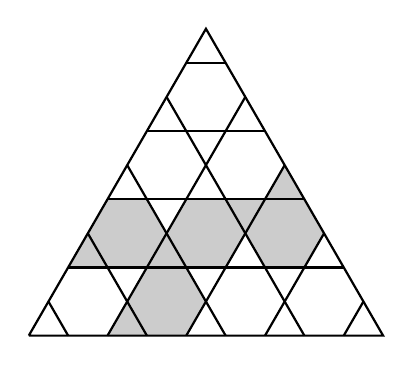
\begin{tikzpicture}
    %polyform
    \filldraw[gray!40] (0.5,0.866) -- (1,0.866) -- (0.75,1.299) -- cycle;
    \filldraw[gray!40] (1,0) -- (1.5,0) -- (1.25,0.433) -- cycle;
    \filldraw[gray!40] (1.5,0) -- (2,0) -- (2.25,0.433) -- (2,0.866) -- (1.5,0.866) -- (1.25,0.433) -- cycle;
    \filldraw[gray!40] (1.5,0.866) -- (2,0.866) -- (1.75,1.299) -- cycle;
    \filldraw[gray!40] (1,0.866) -- (1.5,0.866) -- (1.75,1.299) -- (1.5,1.732) -- (1,1.732) -- (0.75,1.299) -- cycle;
    \filldraw[gray!40] (2,0.866) -- (2.5,0.866) -- (2.75,1.299) -- (2.5,1.732) -- (2,1.732) -- (1.75,1.299) -- cycle;
    \filldraw[gray!40] (2.75,1.299) -- (2.5,1.732) -- (3.25,1.732);
    \filldraw[gray!40] (3,0.866) -- (3.5,0.866) --  (3.75,1.299) -- (3.5,1.732) -- (3,1.732) -- (2.75,1.299) -- cycle;
    \filldraw[gray!40] (3.5,1.732) -- (3,1.732) -- (3.25,2.165) -- cycle;
    
    %lattice
    \draw[thick] (0,0) -- (4.5,0) -- (2.25, 3.897) -- (0,0);
    \draw[thick] (1,0) -- (2.75,3.031);
    \draw[thick] (2,0) -- (3.25,2.165);
    \draw[thick] (3,0) -- (3.75,1.299);
    \draw[thick] (4,0) -- (4.25,0.433);
    
    \draw[thick] (3.5,0) -- (1.75,3.031);
    \draw[thick] (2.5,0) -- (1.25,2.165);
    \draw[thick] (1.5,0) -- (0.75,1.299);
    \draw[thick] (0.5,0) -- (0.25,0.433);
    
    \draw[thick] (0.5,0.866) -- (4,0.866);
    \draw[thick] (1,1.732) -- (3.5,1.732);
    \draw[thick] (1.5,2.598) -- (3,2.598);
    \draw[thick] (2,3.464) -- (2.5,3.464);
    
    \end{tikzpicture}
    %\label{fig:labelled dual of triangle in tri/hex}
\end{minipage}
\captionof{figure}{Polyforms in $S_1$, $S_2$, and $S_3$}
%\caption{fig:something}
\end{center}

\textbf{\textit{Case 1}} Similar to the proof of Theorem \ref{thm: tri in tri}, we use the binomial theorem to get $C(1)=1$ and $C(n) = 2^{2n-3}$ for $n \geq 2$, and consequently $|S_1| = 3(2^{2n-3} -2^{n-2})$. We introduce a new function $H(n)=C(n) -1 -\sum_{k=2}^{n-1}C(k)$. $H(n)$ counts all of the polyforms that are counted in $C(n)$ that do not contain any other cells on one of the shared sides. For example, in Figure \ref{fig: bowtie lattice n is 3}, $H(3)$ is the number of polyforms that contains the node labelled $\{1,3\}$, but not the node labelled $\{3\}$ or $\{2,3\}$. $H$ is used to build the sums in case 2.

\textbf{\textit{Case 2}} Similar to the proof of Theorem \ref{thm: tri in tri}, we next consider the ``U''-shapes that appear in $S_2$ and introduce $E(n)$ to count the number of these ``U'' shapes on a given side. In this lattice we need to split $E(n)$ into two parts $E_1$ and $E_2$. $E_1$ counts the polyforms with ``U''-shapes that only contain $1$ of the triangles that make up the bottom edge, while $E_2$ counts the number of polyforms that contain $2$ or more triangles.

\begin{center}
\begin{minipage}{0.5\textwidth}
    \centering
    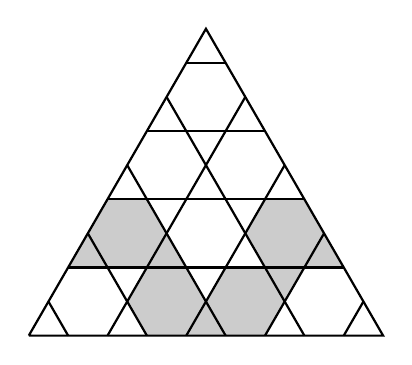
\begin{tikzpicture}
    %polyform
    \filldraw[gray!40] (1.5,0) -- (2,0) -- (2.25,0.433) -- (2,0.866) -- (1.5,0.866) -- (1.25,0.433) -- cycle;
    \filldraw[gray!40] (2,0) -- (2.5,0) -- (2.25,0.433) -- cycle;
    \filldraw[gray!40] (2.5,0) -- (3,0) -- (3.25,0.433) -- (3,0.866) -- (2.5,0.866) -- (2.25,0.433) -- cycle;
    \filldraw[gray!40] (1.5,0.866) -- (2,0.866) -- (1.75,1.299) -- cycle;
    \filldraw[gray!40] (1,0.866) -- (1.5,0.866) -- (1.75,1.299) -- (1.5,1.732) -- (1,1.732) -- (0.75,1.299) -- cycle;
    \filldraw[gray!40] (0.5,0.866) -- (1,0.866) -- (0.75,1.299) -- cycle;
    \filldraw[gray!40] (3.25,0.433) -- (3,0.866) -- (3.5,0.866) -- cycle;
    \filldraw[gray!40] (2.5,0) -- (3,0) -- (3.25,0.433) -- (3,0.866) -- (2.5,0.866) -- (2.25,0.433) -- cycle;
    \filldraw[gray!40] (3.5,0.866) -- (4,0.866) -- (3.75,1.299) -- cycle;
    \filldraw[gray!40] (3,0.866) -- (3.5,0.866) --  (3.75,1.299) -- (3.5,1.732) -- (3,1.732) -- (2.75,1.299) -- cycle;
    
    %lattice
    \draw[thick] (0,0) -- (4.5,0) -- (2.25, 3.897) -- (0,0);
    \draw[thick] (1,0) -- (2.75,3.031);
    \draw[thick] (2,0) -- (3.25,2.165);
    \draw[thick] (3,0) -- (3.75,1.299);
    \draw[thick] (4,0) -- (4.25,0.433);
    
    \draw[thick] (3.5,0) -- (1.75,3.031);
    \draw[thick] (2.5,0) -- (1.25,2.165);
    \draw[thick] (1.5,0) -- (0.75,1.299);
    \draw[thick] (0.5,0) -- (0.25,0.433);
    
    \draw[thick] (0.5,0.866) -- (4,0.866);
    \draw[thick] (1,1.732) -- (3.5,1.732);
    \draw[thick] (1.5,2.598) -- (3,2.598);
    \draw[thick] (2,3.464) -- (2.5,3.464);
    
    \end{tikzpicture}
\end{minipage}\hfill
\begin{minipage}{0.5\textwidth}
    \centering
    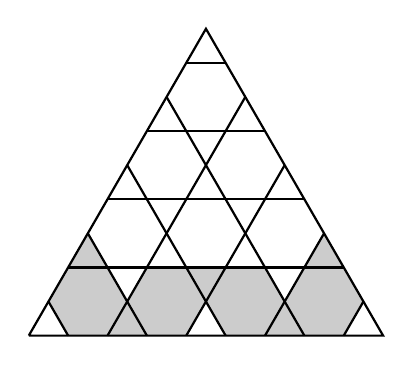
\begin{tikzpicture}
    %polyform
    \filldraw[gray!40] (0.5,0) -- (1,0) -- (1.25,0.433) -- (1,0.866) -- (0.5,0.866) -- (0.25,0.433) -- cycle;
    \filldraw[gray!40] (1,0) -- (1.5,0) -- (1.25,0.433) -- cycle;
    \filldraw[gray!40] (1.5,0) -- (2,0) -- (2.25,0.433) -- (2,0.866) -- (1.5,0.866) -- (1.25,0.433) -- cycle;
    \filldraw[gray!40] (2,0.866) -- (2.5,0.866) -- (2.25,0.433) -- cycle;
    \filldraw[gray!40] (2.5,0) -- (3,0) -- (3.25,0.433) -- (3,0.866) -- (2.5,0.866) -- (2.25,0.433) -- cycle;
    \filldraw[gray!40] (0.5,0.866) -- (1,0.866) -- (0.75,1.299) -- cycle;
    \filldraw[gray!40] (3,0) -- (3.5,0) -- (3.25,0.433) -- cycle;
    \filldraw[gray!40] (3.5,0) -- (4,0) -- (4.25,0.433) -- (4,0.866) -- (3.5,0.866) -- (3.25,0.433) -- cycle;
    \filldraw[gray!40] (3.5,0.866) -- (4,0.866) -- (3.75,1.299) -- cycle;
    
    %lattice
    \draw[thick] (0,0) -- (4.5,0) -- (2.25, 3.897) -- (0,0);
    \draw[thick] (1,0) -- (2.75,3.031);
    \draw[thick] (2,0) -- (3.25,2.165);
    \draw[thick] (3,0) -- (3.75,1.299);
    \draw[thick] (4,0) -- (4.25,0.433);
    
    \draw[thick] (3.5,0) -- (1.75,3.031);
    \draw[thick] (2.5,0) -- (1.25,2.165);
    \draw[thick] (1.5,0) -- (0.75,1.299);
    \draw[thick] (0.5,0) -- (0.25,0.433);
    
    \draw[thick] (0.5,0.866) -- (4,0.866);
    \draw[thick] (1,1.732) -- (3.5,1.732);
    \draw[thick] (1.5,2.598) -- (3,2.598);
    \draw[thick] (2,3.464) -- (2.5,3.464);
    
    \end{tikzpicture}
\end{minipage}

\captionof{figure}{Polyforms counted by $E_1$ and $E_2$}
\end{center}

We number the triangles that belong to the bottom edge $1$ to $n$ from left to right. Polyforms that have the ``U'' shape with one triangle can be found at cells $2$ through $n-1$. This gives
$$E_1(n) = \sum_{i=2}^{n-1}H(i)H(n+1-i)$$

For $E_2$, call the leftmost triangle on the bottom row $i$ and the rightmost $j$. There are $i-j-1$ triangles between $i$ and $j$, and so there are $2^{i-j-1}$ different paths between the cells $i$ and $j$. This gives
$$E_2(n) = \sum_{i=2}^{n-2}\sum_{j=i+1}^{n-1}2^{j-i-1}H(i)H(n+1-j).$$

Therefore $|S_2| = 3E(n) = 3E_1(n)+3E_2(n).$

\textbf{\textit{Case 3}} In a similar fashion to Theorem \ref{thm: tri in tri} we see that $|S_3| = I(n) = (n-2)(n-3)2^{2n-4}.$

Solving the sums in case 2 and combining $|S_1|$, $|S_2|$, and $|S_3|$ gives the result.

\end{proof}

The first terms of this sequence, for $n \geq 2$, starts $3, 21, 125, 693, 3669, 18733, \dots$ (A356889 \cite{oeis})

Theorem \ref{thm:tri in tri hex} can be extended by adding $a-2$ additional edges in a symmetric manner, shown in Figure \ref{fig:extended tri hex}. We will call the family of these graphs $\triangle^{K,a}_n$, where $K,a$ represents the dual with $a$ connections, and $n$ represents the size. 

\begin{center}
\begin{minipage}{0.45\textwidth}
\centering
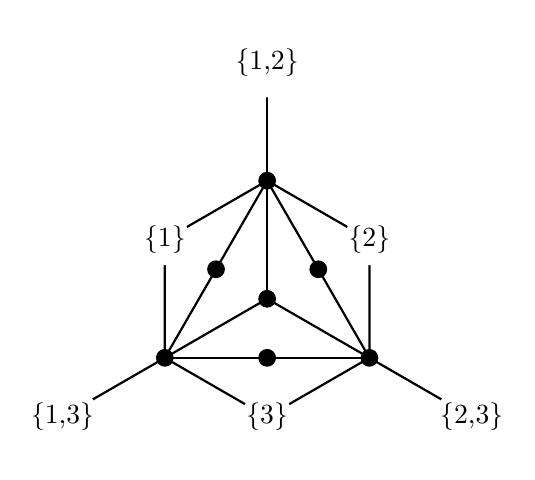
\begin{tikzpicture}
%edges
\draw[thick] (0,0) -- (1.299,0.75);
\draw[thick] (5.196,0) -- (3.897,0.75);
\draw[thick] (2.598,3) -- (2.598,4.5);

\draw[thick] (1.299,0.75) -- (2.598,0) -- (3.897,0.75) -- (3.897,2.25) -- (2.598,3) -- (1.299,2.25) -- (1.299,0.75);
\draw[thick] (1.299,0.75) -- (2.598, 1.5) -- (3.897,0.75);
\draw[thick] (2.598,3) -- (2.598, 1.5);
% (1.299,0.75) and (2.598,3) gives (1.949,1.875)
% (3.897,0.75) and (2.598,3) gives (3.248,1.875)
% (1.299,0.75) and (3.897,0.75) gives (2.598,0.75)
\draw[thick] (1.299,0.75) -- (1.949,1.875) -- (2.598,3);

\draw[thick] (3.897,0.75) -- (3.248,1.875) -- (2.598,3);

\draw[thick] (1.299,0.75) -- (2.598,0.75) -- (3.897,0.75);


%nodes
\( \lablnode{0}{0}{1,3} \)
\( \lablnode{2.598}{0}{3} \)
\draw[fill=black] (1.299,0.75) circle (3pt);
\( \lablnode{1.299}{2.25}{1} \)
\draw[fill=black] (3.897,0.75) circle (3pt);
\( \lablnode{5.196}{0}{2,3} \)
\( \lablnode{3.897}{2.25}{2} \)
\draw[fill=black] (2.598,3) circle (3pt);
\( \lablnode{2.598}{4.5}{1,2} \)
\draw[fill=black] (2.598,1.5) circle (3pt);

\draw[fill=black] (1.949,1.875) circle (3pt);
\draw[fill=black] (3.248,1.875) circle (3pt);
\draw[fill=black] (2.598,0.75) circle (3pt);

\end{tikzpicture}
\end{minipage}\hfill
\begin{minipage}{0.45\textwidth}
\centering
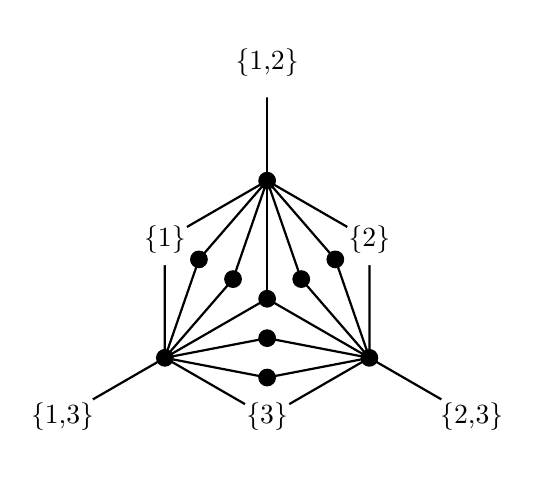
\begin{tikzpicture}
%edges
\draw[thick] (0,0) -- (1.299,0.75);
\draw[thick] (5.196,0) -- (3.897,0.75);
\draw[thick] (2.598,3) -- (2.598,4.5);

\draw[thick] (1.299,0.75) -- (2.598,0) -- (3.897,0.75) -- (3.897,2.25) -- (2.598,3) -- (1.299,2.25) -- (1.299,0.75);
\draw[thick] (1.299,0.75) -- (2.598, 1.5) -- (3.897,0.75);
\draw[thick] (2.598,3) -- (2.598, 1.5);
% (1.299,2.25) and (2.598, 1.5)
\draw[thick] (1.299,0.75) -- (1.732,2) -- (2.598,3);
\draw[thick] (1.299,0.75) -- (2.165,1.75) -- (2.598,3);

\draw[thick] (3.897,0.75) -- (3.031,1.75) -- (2.598,3);
\draw[thick] (3.897,0.75) -- (3.464,2) -- (2.598,3);

\draw[thick] (1.299,0.75) -- (2.598,0.5) -- (3.897,0.75);
\draw[thick] (1.299,0.75) -- (2.598,1) -- (3.897,0.75);

%nodes
\( \lablnode{0}{0}{1,3} \)
\( \lablnode{2.598}{0}{3} \)
\draw[fill=black] (1.299,0.75) circle (3pt);
\( \lablnode{1.299}{2.25}{1} \)
\draw[fill=black] (3.897,0.75) circle (3pt);
\( \lablnode{5.196}{0}{2,3} \)
\( \lablnode{3.897}{2.25}{2} \)
\draw[fill=black] (2.598,3) circle (3pt);
\( \lablnode{2.598}{4.5}{1,2} \)
\draw[fill=black] (2.598,1.5) circle (3pt);

\draw[fill=black] (2.598,0.5) circle (3pt);
\draw[fill=black] (2.598,1) circle (3pt);
\draw[fill=black] (3.031,1.75) circle (3pt);
\draw[fill=black] (3.464,2) circle (3pt);
\draw[fill=black] (1.732,2) circle (3pt);
\draw[fill=black] (2.165,1.75) circle (3pt);

\end{tikzpicture}
\end{minipage}
\captionof{figure}{Duals of $\triangle^{K,3}_3$ and $\triangle^{K,4}_3$}\label{fig:extended tri hex}
\end{center}

Notice that we recover $\triangle^K_n$ for $a=2$. 

\begin{theorem}
For a given $a \geq 2$, the number of minimal inscribed polyforms $\rho(\triangle^{K,a}_n)$ for $n \geq 2$ is given by the following formula.

\begin{equation}
    \rho(\triangle^{K,a}_n) = \left(n^2+\frac{(6a^2-5a-5)n}{a+1} + \frac{6(a^4-2a^3+2a+1)}{(a+1)^2}\right)2^{n-2}a^{n-4}-\frac{3(a-1)^n}{(a+1)^2}
\end{equation}

\end{theorem}

\begin{proof}
    This proof extends the sums of Theorem \ref{thm:tri in tri hex} for a given $a$.

    \textbf{\textit{Case 1}} We parameterize the method in Theorem \ref{thm:tri in tri hex}. We have $C_a(1)=1$, and $C_a(n)=2^{n-1}a^{n-2}$ for $n \geq 2$. This gives $|S_1|=3(C_a(n)-a^{n-2})$. We  $H_a(n) = C_a(n) - (a-1)^{n-2} - \sum_{k=2}^{n-1}(a-1)^{n-1-k}C_a(k)$, which represents all the polyforms counted in $C_a(n)$ that do not contain any other cells on one of the shared sides. For example in Figure \ref{fig:extended tri hex} $H_a(3)$ is the number of polyforms that contains the cell labelled $\{1,3\}$, but not $\{3\}$ or $\{2,3\}$. 

    \textbf{\textit{Case 2}} We form the sums in a similar way to Theorem \ref{thm:tri in tri hex}. $|S_2| = 3E_1(n) + 3E_2(n)$, where
    $$E_{1,a}(n) = \sum_{i=2}^{n-1}H_a(i)H_a(n+1-i)$$

    and
    
    $$E_{2,a}(n) = \sum_{i=1}^{n-2}\sum_{j=i+1}^{n-1}a^{j-i-1}H_a(i)H_a(n+1-j).$$

    \textbf{\textit{Case 3}} Similar to Theorem \ref{thm:tri in tri hex} we have $|S_3| = I_a(n) = (n-2)(n-3)2^{n-2}a^{n-4}.$ 

    Solving the sums in case 2 and combining $|S_1|, |S_2|$, and $|S_3|$ gives the result.
\end{proof}

Interestingly, though initially defined for $a \geq 2$, $\rho(\triangle^{K,1}_n) =  ((n-1)^2  + 2)2^{n-2} = \rho(\triangle^{T}_n)$. So in the case of minimal inscribed polyforms $\triangle^{T}_n$ can be seen as the $a=1$ case of $\triangle^{K,a}_n$

\subsection{Minimal Inscribed Polyforms in \texorpdfstring{$\mathbf{\triangle^{H*}_n}$}{H*n}}

Different labellings of the same lattice can also give interesting results. 

\begin{center}
    \begin{minipage}{0.25\textwidth}
        \centering
        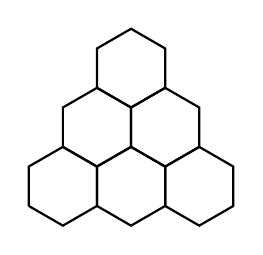
\begin{tikzpicture}
        %lattice
        \draw[thick] (0,0.25) -- (0.433,0) -- (0.866,0.25) -- (0.866,0.75) -- (0.433,1) -- (0,0.75) -- (0,0.25);
        \draw[thick] (0.866,0.25) -- (1.299,0) -- (1.732,0.25) -- (1.732,0.75) -- (1.299,1) -- (0.866,0.75) -- (0.866,0.25);
        \draw[thick] (1.732,0.25) -- (2.165,0) -- (2.598,0.25) -- (2.598,0.75) -- (2.165,1) -- (1.732,0.75) -- (1.732,0.25);
        
        \draw[thick] (0.433,1) -- (0.866,0.75) -- (1.299,1) -- (1.299,1.5) -- (0.866,1.75) -- (0.433,1.5) -- (0.433,1);
        \draw[thick] (1.299,1) -- (1.732,0.75) -- (2.165,1) -- (2.165,1.5) -- (1.732,1.75) -- (1.299,1.5) -- (1.299,1);
        
        \draw[thick] (0.866,1.75) -- (1.299,1.5) -- (1.732,1.75) -- (1.732,2.25) -- (1.299,2.5) -- (0.866,2.25) -- (0.866,1.75);
        \end{tikzpicture}
    \end{minipage}\hfill
    \begin{minipage}{0.25\textwidth}
        \centering
        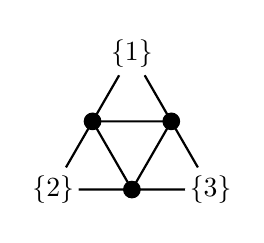
\begin{tikzpicture}
        %edges
        \draw[thick] (0,0) -- (1,0) -- (2,0) -- (1.5,0.866) -- (1,1.732) -- (0.5,0.866);
        \draw[thick] (0.5,0.866) -- (1.5, 0.866) -- (1,0) -- (0.5,0.866) -- (0,0);
        %nodes
        \( \lablnode{0}{0}{2} \)
        \( \lablnode{2}{0}{3} \)
        \( \lablnode{1}{1.732}{1} \)
        \draw[fill=black] (1,0) circle (3pt);
        \draw[fill=black] (0.5,0.866) circle (3pt);
        \draw[fill=black] (1.5,0.866) circle (3pt);
        \end{tikzpicture}
    \end{minipage}\hfill
    \begin{minipage}{0.25\textwidth}
        \centering
        \begin{tikzpicture}
        %polyform
        %\filldraw[gray!40] (0,0.25) -- (0.433,0) -- (0.866,0.25) -- (0.866,0.75) -- (0.433,1) -- (0,0.75) -- (0,0.25);
        \filldraw[gray!40] (0,0.25) -- (0.433,0) -- (0.866,0.25) -- (1.299,0) -- (1.732,0.25) -- (1.732,0.75) -- (2.165,1) -- (2.165,1.5) -- (1.732,1.75) -- (1.299,1.5) -- (1.299,1) -- (0.866,0.75) -- (0.433,1) -- (0,0.75) -- (0,0.25);
        \filldraw[gray!40] (1.732,0.25) -- (2.165,0) -- (2.598,0.25) -- (2.598,0.75) -- (2.165,1) -- (1.732,0.75) -- (1.732,0.25);
        \filldraw[gray!40] (0.866,1.75) -- (1.299,1.5) -- (1.732,1.75) -- (1.732,2.25) -- (1.299,2.5) -- (0.866,2.25) -- (0.866,1.75);
        %lattice
        \draw[thick] (0,0.25) -- (0.433,0) -- (0.866,0.25) -- (0.866,0.75) -- (0.433,1) -- (0,0.75) -- (0,0.25);
        \draw[thick] (0.866,0.25) -- (1.299,0) -- (1.732,0.25) -- (1.732,0.75) -- (1.299,1) -- (0.866,0.75) -- (0.866,0.25);
        \draw[thick] (1.732,0.25) -- (2.165,0) -- (2.598,0.25) -- (2.598,0.75) -- (2.165,1) -- (1.732,0.75) -- (1.732,0.25);
        
        \draw[thick] (0.433,1) -- (0.866,0.75) -- (1.299,1) -- (1.299,1.5) -- (0.866,1.75) -- (0.433,1.5) -- (0.433,1);
        \draw[thick] (1.299,1) -- (1.732,0.75) -- (2.165,1) -- (2.165,1.5) -- (1.732,1.75) -- (1.299,1.5) -- (1.299,1);
        
        \draw[thick] (0.866,1.75) -- (1.299,1.5) -- (1.732,1.75) -- (1.732,2.25) -- (1.299,2.5) -- (0.866,2.25) -- (0.866,1.75);
        \end{tikzpicture}
    \end{minipage}
    \captionof{figure}{The tiling and dual representation of $\triangle^{H*}_3$ and an example polyform}\label{fig:tri in hex extendo}
\end{center}

Let us call the family shown in Figure \ref{fig:tri in hex extendo} $\triangle^{H*}_n$, where $H*$ indicates an alternative labelling of the hexagonal lattice. Here $k=3$ and $m(\triangle^{H*}_n) = 2n-1$.

\begin{theorem}\label{thm: tri in hex ex}
The number of minimal inscribed polyforms $\rho(\triangle^{H*}_n)$ for $n\geq 2$ is given by the following formula.

\begin{equation}\label{eq: tri in hexagons}
    \rho(\triangle^{H*}_n) = \binom{2(n-1)}{n-1} - \sum_{k=0}^{n-2}\binom{2k}{k}.
\end{equation}
\end{theorem}

\begin{proof}
Each unit hexagon in the triangle corresponds with a unique weak integer $3$-composition of $n-1$. Figure \ref{fig: Int Composition} shows the visual interpretation of the integer composition for the dark grey hexagon. The lengths of the $3$ light grey ``spokes" are the components of the composition. Suppose the components of the composition are labelled $k_1$, $k_2$, and $k_3$. Then Figure \ref{fig: Int Composition} represents the cell for $k_1 = 2$, $k_2 = 1$, and $k_3 = 1$, read counter-clockwise around the dark grey hexagon. 

\begin{center}
\centering
\begin{tikzpicture}
    %polyform
\filldraw[gray!40] (1.732,0.25) -- (2.165,0) -- (2.598,0.25) -- (2.598,0.75) -- (2.165,1) -- (1.732,0.75) -- (1.732,0.25);

\filldraw[gray!95] (2.165,1) -- (2.598,0.75) -- (3.031,1) -- (3.031,1.5) -- (2.598,1.75) -- (2.165,1.5) -- (2.165,1);
\filldraw[gray!40] (3.031,1) -- (3.464,0.75) -- (3.897,1) -- (3.897,1.5) -- (3.464,1.75) -- (3.031,1.5) -- (3.031,1);

\filldraw[gray!40] (1.732,1.75) -- (2.165,1.5) -- (2.598,1.75) -- (2.598,2.25) -- (2.165,2.5) -- (1.732,2.25) -- (1.732,1.75);

\filldraw[gray!40] (1.299,2.5) -- (1.732,2.25) -- (2.165,2.5) -- (2.165,3) -- (1.732,3.25) -- (1.299,3) -- (1.299,2.5);

%row 1
\draw[thick] (0,0.25) -- (0.433,0) -- (0.866,0.25) -- (0.866,0.75) -- (0.433,1) -- (0,0.75) -- (0,0.25);
\draw[thick] (0.866,0.25) -- (1.299,0) -- (1.732,0.25) -- (1.732,0.75) -- (1.299,1) -- (0.866,0.75) -- (0.866,0.25);
\draw[thick] (1.732,0.25) -- (2.165,0) -- (2.598,0.25) -- (2.598,0.75) -- (2.165,1) -- (1.732,0.75) -- (1.732,0.25);

\draw[thick] (2.598,0.25) -- (3.031,0) -- (3.464,0.25) -- (3.464,0.75) -- (3.031,1) -- (2.598,0.75) -- (2.598,0.25);
\draw[thick] (3.464,0.25) -- (3.897,0) -- (4.33,0.25) -- (4.33,0.75) -- (3.897,1) -- (3.464,0.75) -- (3.464,0.25);

%row 2
\draw[thick] (0.433,1) -- (0.866,0.75) -- (1.299,1) -- (1.299,1.5) -- (0.866,1.75) -- (0.433,1.5) -- (0.433,1);
\draw[thick] (1.299,1) -- (1.732,0.75) -- (2.165,1) -- (2.165,1.5) -- (1.732,1.75) -- (1.299,1.5) -- (1.299,1);
\draw[thick] (2.165,1) -- (2.598,0.75) -- (3.031,1) -- (3.031,1.5) -- (2.598,1.75) -- (2.165,1.5) -- (2.165,1);
\draw[thick] (3.031,1) -- (3.464,0.75) -- (3.897,1) -- (3.897,1.5) -- (3.464,1.75) -- (3.031,1.5) -- (3.031,1);

%row 3
\draw[thick] (0.866,1.75) -- (1.299,1.5) -- (1.732,1.75) -- (1.732,2.25) -- (1.299,2.5) -- (0.866,2.25) -- (0.866,1.75);
\draw[thick] (1.732,1.75) -- (2.165,1.5) -- (2.598,1.75) -- (2.598,2.25) -- (2.165,2.5) -- (1.732,2.25) -- (1.732,1.75);
\draw[thick] (2.598,1.75) -- (3.031,1.5) -- (3.464,1.75) -- (3.464,2.25) -- (3.031,2.5) -- (2.598,2.25) -- (2.598,1.75);

%row 4
\draw[thick] (1.299,2.5) -- (1.732,2.25) -- (2.165,2.5) -- (2.165,3) -- (1.732,3.25) -- (1.299,3) -- (1.299,2.5);
\draw[thick] (2.165,2.5) -- (2.598,2.25) -- (3.031,2.5) -- (3.031,3) -- (2.598,3.25) -- (2.165,3) -- (2.165,2.5);

%row 5
\draw[thick] (1.732,3.25) -- (2.165,3) -- (2.598,3.25) -- (2.598,3.75) -- (2.165,4) -- (1.732,3.75) -- (1.732,3.25);

\end{tikzpicture}
%\label{fig:dual 3 triangle2}

\captionof{figure}{A cell with spokes}\label{fig: Int Composition}
%\label{fig:dual 3 triangle2}
\end{center}

Notice that $k_i$ can be $0$, as there are cells in which one cannot extend a spoke in a certain direction (the dark grey hexagon being located on a side or corner). 

Using the spokes as guides, we can group paths from each corner to the dark grey hexagon. An example of this grouping is shown in Figure \ref{fig: Int Composition Grouping}.

\begin{center}
\centering
\begin{tikzpicture}
    %polyform

\filldraw[gray!60] (0,0.25) -- (0.433,0) -- (0.866,0.25) -- (1.299,0) -- (1.732,0.25) -- (2.165,0) -- (2.598,0.25)-- (2.598,0.75) -- (3.031,1) -- (3.031,1.5) -- (2.598,1.75) -- (2.165,1.5) -- (1.732,1.75) -- (1.299,1.5)  -- (0.866,1.75)-- (0.433,1.5) -- (0.433,1) -- (0.433,1) -- (0,0.75)  -- (0,0.25);

\filldraw[gray!20] (2.165,1.5) -- (2.165,1) -- (2.598,0.75) -- (2.598,0.25) -- (3.031,0) -- (3.464,0.25) -- (3.897,0) -- (4.33,0.25) -- (4.33,0.75) -- (3.897,1) -- (3.897, 1.5) -- (3.464,1.75) -- (3.031,1.5) -- (3.031,1);

\filldraw[gray!40] (3.464,1.75) -- (3.464,2.25) -- (3.031,2.5) -- (3.031,3) -- (2.598,3.25) -- (2.598,3.25) -- (2.598,3.75) -- (2.165,4) -- (1.732,3.75) -- (1.732,3.25) -- (1.732,3.25) -- (1.299,3) -- (1.299,2.5) -- (1.732, 2.25) -- (1.732, 1.75) -- (2.165,1.5) -- (2.598,1.75) -- (3.031,1.5) -- (3.464,1.75);

\filldraw[gray!95] (2.165,1) -- (2.598,0.75) -- (3.031,1) -- (3.031,1.5) -- (2.598,1.75) -- (2.165,1.5) -- (2.165,1);

%row 1
\draw[thick] (0,0.25) -- (0.433,0) -- (0.866,0.25) -- (0.866,0.75) -- (0.433,1) -- (0,0.75) -- (0,0.25);
\draw[thick] (0.866,0.25) -- (1.299,0) -- (1.732,0.25) -- (1.732,0.75) -- (1.299,1) -- (0.866,0.75) -- (0.866,0.25);
\draw[thick] (1.732,0.25) -- (2.165,0) -- (2.598,0.25) -- (2.598,0.75) -- (2.165,1) -- (1.732,0.75) -- (1.732,0.25);
\draw[thick] (2.598,0.25) -- (3.031,0) -- (3.464,0.25) -- (3.464,0.75) -- (3.031,1) -- (2.598,0.75) -- (2.598,0.25);
\draw[thick] (3.464,0.25) -- (3.897,0) -- (4.33,0.25) -- (4.33,0.75) -- (3.897,1) -- (3.464,0.75) -- (3.464,0.25);

%row 2
\draw[thick] (0.433,1) -- (0.866,0.75) -- (1.299,1) -- (1.299,1.5) -- (0.866,1.75) -- (0.433,1.5) -- (0.433,1);
\draw[thick] (1.299,1) -- (1.732,0.75) -- (2.165,1) -- (2.165,1.5) -- (1.732,1.75) -- (1.299,1.5) -- (1.299,1);
\draw[thick] (2.165,1) -- (2.598,0.75) -- (3.031,1) -- (3.031,1.5) -- (2.598,1.75) -- (2.165,1.5) -- (2.165,1);
\draw[thick] (3.031,1) -- (3.464,0.75) -- (3.897,1) -- (3.897,1.5) -- (3.464,1.75) -- (3.031,1.5) -- (3.031,1);

%row 3
\draw[thick] (0.866,1.75) -- (1.299,1.5) -- (1.732,1.75) -- (1.732,2.25) -- (1.299,2.5) -- (0.866,2.25) -- (0.866,1.75);
\draw[thick] (1.732,1.75) -- (2.165,1.5) -- (2.598,1.75) -- (2.598,2.25) -- (2.165,2.5) -- (1.732,2.25) -- (1.732,1.75);
\draw[thick] (2.598,1.75) -- (3.031,1.5) -- (3.464,1.75) -- (3.464,2.25) -- (3.031,2.5) -- (2.598,2.25) -- (2.598,1.75);

%row 4
\draw[thick] (1.299,2.5) -- (1.732,2.25) -- (2.165,2.5) -- (2.165,3) -- (1.732,3.25) -- (1.299,3) -- (1.299,2.5);
\draw[thick] (2.165,2.5) -- (2.598,2.25) -- (3.031,2.5) -- (3.031,3) -- (2.598,3.25) -- (2.165,3) -- (2.165,2.5);

%row 5
\draw[thick] (1.732,3.25) -- (2.165,3) -- (2.598,3.25) -- (2.598,3.75) -- (2.165,4) -- (1.732,3.75) -- (1.732,3.25);

%hi light
\draw[line width = 0.4mm, red] (0,0.25) -- (0.433,0) -- (0.866,0.25) -- (1.299,0) -- (1.732,0.25) -- (2.165,0) -- (2.598,0.25)-- (2.598,0.75) -- (3.031,1) -- (3.031,1.5) -- (2.598,1.75) -- (2.165,1.5) -- (1.732,1.75) -- (1.299,1.5)  -- (0.866,1.75)-- (0.433,1.5) -- (0.433,1) -- (0.433,1) -- (0,0.75)  -- (0,0.25);

\draw[line width = 0.4mm, red] (2.165,1.5) -- (2.165,1) -- (2.598,0.75) -- (2.598,0.25) -- (3.031,0) -- (3.464,0.25) -- (3.897,0) -- (4.33,0.25) -- (4.33,0.75) -- (3.897,1) -- (3.897, 1.5) -- (3.464,1.75) -- (3.031,1.5) -- (3.031,1);

\draw[line width = 0.4mm, red] (3.464,1.75) -- (3.464,2.25) -- (3.031,2.5) -- (3.031,3) -- (2.598,3.25) -- (2.598,3.25) -- (2.598,3.75) -- (2.165,4) -- (1.732,3.75) -- (1.732,3.25) -- (1.732,3.25) -- (1.299,3) -- (1.299,2.5) -- (1.732, 2.25) -- (1.732, 1.75);

\end{tikzpicture}
%\label{fig:dual 3 triangle2}

\captionof{figure}{A cell in the $n=5$ triangle with groupings}\label{fig: Int Composition Grouping}
%\label{fig:dual 3 triangle2}
\end{center}

Using this grouping we can construct the following sum for the number of possible sets of paths from each corner to a given vertex.

\begin{equation}\label{eq: naiive sum}
    s(n) = \sum_{k_1 + k_2 + k_3 = n-1} \binom{k_1 + k_2}{k_1}\binom{k_2+k_3}{k_2}\binom{k_3+k_1}{k_3}
\end{equation}

Notice that this grouping, and consequently $s(n)$, will count certain polyforms multiple times. An example of a polyform that is counted multiple times is shown in Figure \ref{fig: Double Count}.

\begin{center}
\centering
\begin{tikzpicture}
    %polyform
\filldraw[gray!40] (0,0.25) -- (0.433,0) -- (0.866,0.25) -- (0.866,0.75) -- (0.433,1) -- (0,0.75) -- (0,0.25);

\filldraw[gray!40] (0.866,0.25) -- (1.299,0) -- (1.732,0.25) -- (1.732,0.75) -- (1.299,1) -- (0.866,0.75) -- (0.866,0.25);

\filldraw[gray!40] (3.464,0.25) -- (3.897,0) -- (4.33,0.25) -- (4.33,0.75) -- (3.897,1) -- (3.464,0.75) -- (3.464,0.25);

\filldraw[gray!40] (1.299,1) -- (1.732,0.75) -- (2.165,1) -- (2.165,1.5) -- (1.732,1.75) -- (1.299,1.5) -- (1.299,1);
\filldraw[gray!40] (2.165,1) -- (2.598,0.75) -- (3.031,1) -- (3.031,1.5) -- (2.598,1.75) -- (2.165,1.5) -- (2.165,1);
\filldraw[gray!40] (3.031,1) -- (3.464,0.75) -- (3.897,1) -- (3.897,1.5) -- (3.464,1.75) -- (3.031,1.5) -- (3.031,1);
\filldraw[gray!40] (1.732,1.75) -- (2.165,1.5) -- (2.598,1.75) -- (2.598,2.25) -- (2.165,2.5) -- (1.732,2.25) -- (1.732,1.75);
\filldraw[gray!40] (1.299,2.5) -- (1.732,2.25) -- (2.165,2.5) -- (2.165,3) -- (1.732,3.25) -- (1.299,3) -- (1.299,2.5);
\filldraw[gray!40] (1.732,3.25) -- (2.165,3) -- (2.598,3.25) -- (2.598,3.75) -- (2.165,4) -- (1.732,3.75) -- (1.732,3.25);

%row 1
\draw[thick] (0,0.25) -- (0.433,0) -- (0.866,0.25) -- (0.866,0.75) -- (0.433,1) -- (0,0.75) -- (0,0.25);
\draw[thick] (0.866,0.25) -- (1.299,0) -- (1.732,0.25) -- (1.732,0.75) -- (1.299,1) -- (0.866,0.75) -- (0.866,0.25);
\draw[thick] (1.732,0.25) -- (2.165,0) -- (2.598,0.25) -- (2.598,0.75) -- (2.165,1) -- (1.732,0.75) -- (1.732,0.25);
\draw[thick] (2.598,0.25) -- (3.031,0) -- (3.464,0.25) -- (3.464,0.75) -- (3.031,1) -- (2.598,0.75) -- (2.598,0.25);
\draw[thick] (3.464,0.25) -- (3.897,0) -- (4.33,0.25) -- (4.33,0.75) -- (3.897,1) -- (3.464,0.75) -- (3.464,0.25);

%row 2
\draw[thick] (0.433,1) -- (0.866,0.75) -- (1.299,1) -- (1.299,1.5) -- (0.866,1.75) -- (0.433,1.5) -- (0.433,1);
\draw[thick] (1.299,1) -- (1.732,0.75) -- (2.165,1) -- (2.165,1.5) -- (1.732,1.75) -- (1.299,1.5) -- (1.299,1);
\draw[thick] (2.165,1) -- (2.598,0.75) -- (3.031,1) -- (3.031,1.5) -- (2.598,1.75) -- (2.165,1.5) -- (2.165,1);
\draw[thick] (3.031,1) -- (3.464,0.75) -- (3.897,1) -- (3.897,1.5) -- (3.464,1.75) -- (3.031,1.5) -- (3.031,1);

%row 3
\draw[thick] (0.866,1.75) -- (1.299,1.5) -- (1.732,1.75) -- (1.732,2.25) -- (1.299,2.5) -- (0.866,2.25) -- (0.866,1.75);
\draw[thick] (1.732,1.75) -- (2.165,1.5) -- (2.598,1.75) -- (2.598,2.25) -- (2.165,2.5) -- (1.732,2.25) -- (1.732,1.75);
\draw[thick] (2.598,1.75) -- (3.031,1.5) -- (3.464,1.75) -- (3.464,2.25) -- (3.031,2.5) -- (2.598,2.25) -- (2.598,1.75);

%row 4
\draw[thick] (1.299,2.5) -- (1.732,2.25) -- (2.165,2.5) -- (2.165,3) -- (1.732,3.25) -- (1.299,3) -- (1.299,2.5);
\draw[thick] (2.165,2.5) -- (2.598,2.25) -- (3.031,2.5) -- (3.031,3) -- (2.598,3.25) -- (2.165,3) -- (2.165,2.5);

%row 5
\draw[thick] (1.732,3.25) -- (2.165,3) -- (2.598,3.25) -- (2.598,3.75) -- (2.165,4) -- (1.732,3.75) -- (1.732,3.25);

\end{tikzpicture}
%\label{fig:dual 3 triangle2}

\captionof{figure}{A minimal inscribed polyform that is counted multiple times}\label{fig: Double Count}
%\label{fig:dual 3 triangle2}
\end{center}

All polyforms that are grouped multiple ways contains the following substructure.

\begin{center}
\centering
\begin{tikzpicture}
    %polyform
\filldraw[gray!40] (0,0.25) -- (0.433,0) -- (0.866,0.25) -- (0.866,0.75) -- (0.433,1) -- (0,0.75) -- (0,0.25);
\filldraw[gray!40]  (0.866,0.25) -- (1.299,0) -- (1.732,0.25) -- (1.732,0.75) -- (1.299,1) -- (0.866,0.75) -- (0.866,0.25);
\filldraw[gray!40] (0.433,1) -- (0.866,0.75) -- (1.299,1) -- (1.299,1.5) -- (0.866,1.75) -- (0.433,1.5) -- (0.433,1);

%row 1
\draw[thick] (0,0.25) -- (0.433,0) -- (0.866,0.25) -- (0.866,0.75) -- (0.433,1) -- (0,0.75) -- (0,0.25);
\draw[thick] (0.866,0.25) -- (1.299,0) -- (1.732,0.25) -- (1.732,0.75) -- (1.299,1) -- (0.866,0.75) -- (0.866,0.25);

%row 2
\draw[thick] (0.433,1) -- (0.866,0.75) -- (1.299,1) -- (1.299,1.5) -- (0.866,1.75) -- (0.433,1.5) -- (0.433,1);

\end{tikzpicture}
%\label{fig:dual 3 triangle2}

\captionof{figure}{The substructure that allows for multiple groupings.}\label{fig: multi focal point}
%\label{fig:dual 3 triangle2}
\end{center}

Polyforms with these substructures are counted $3$ separate times. Fortunately, the number of polyforms that contain this substructure are easy to count, after the following transformation is made.

\begin{center}
\begin{minipage}{0.45\textwidth}
\centering
    \begin{tikzpicture}
    \filldraw[gray!40] (0,0.25) -- (0.433,0) -- (0.866,0.25) -- (0.866,0.75) -- (0.433,1) -- (0,0.75) -- (0,0.25);

\filldraw[gray!40] (0.866,0.25) -- (1.299,0) -- (1.732,0.25) -- (1.732,0.75) -- (1.299,1) -- (0.866,0.75) -- (0.866,0.25);

\filldraw[gray!40] (3.464,0.25) -- (3.897,0) -- (4.33,0.25) -- (4.33,0.75) -- (3.897,1) -- (3.464,0.75) -- (3.464,0.25);

\filldraw[gray!95] (1.299,1) -- (1.732,0.75) -- (2.165,1) -- (2.165,1.5) -- (1.732,1.75) -- (1.299,1.5) -- (1.299,1);
\filldraw[gray!95] (2.165,1) -- (2.598,0.75) -- (3.031,1) -- (3.031,1.5) -- (2.598,1.75) -- (2.165,1.5) -- (2.165,1);
\filldraw[gray!40] (3.031,1) -- (3.464,0.75) -- (3.897,1) -- (3.897,1.5) -- (3.464,1.75) -- (3.031,1.5) -- (3.031,1);
\filldraw[gray!95] (1.732,1.75) -- (2.165,1.5) -- (2.598,1.75) -- (2.598,2.25) -- (2.165,2.5) -- (1.732,2.25) -- (1.732,1.75);
\filldraw[gray!40] (1.299,2.5) -- (1.732,2.25) -- (2.165,2.5) -- (2.165,3) -- (1.732,3.25) -- (1.299,3) -- (1.299,2.5);
\filldraw[gray!40] (1.732,3.25) -- (2.165,3) -- (2.598,3.25) -- (2.598,3.75) -- (2.165,4) -- (1.732,3.75) -- (1.732,3.25);
    
    %row 1
    \draw[thick] (0,0.25) -- (0.433,0) -- (0.866,0.25) -- (0.866,0.75) -- (0.433,1) -- (0,0.75) -- (0,0.25);
    \draw[thick] (0.866,0.25) -- (1.299,0) -- (1.732,0.25) -- (1.732,0.75) -- (1.299,1) -- (0.866,0.75) -- (0.866,0.25);
    \draw[thick] (1.732,0.25) -- (2.165,0) -- (2.598,0.25) -- (2.598,0.75) -- (2.165,1) -- (1.732,0.75) -- (1.732,0.25);
    
    \draw[thick] (2.598,0.25) -- (3.031,0) -- (3.464,0.25) -- (3.464,0.75) -- (3.031,1) -- (2.598,0.75) -- (2.598,0.25);
    \draw[thick] (3.464,0.25) -- (3.897,0) -- (4.33,0.25) -- (4.33,0.75) -- (3.897,1) -- (3.464,0.75) -- (3.464,0.25);
    
    %row 2
    \draw[thick] (0.433,1) -- (0.866,0.75) -- (1.299,1) -- (1.299,1.5) -- (0.866,1.75) -- (0.433,1.5) -- (0.433,1);
    \draw[thick] (1.299,1) -- (1.732,0.75) -- (2.165,1) -- (2.165,1.5) -- (1.732,1.75) -- (1.299,1.5) -- (1.299,1);
    \draw[thick] (2.165,1) -- (2.598,0.75) -- (3.031,1) -- (3.031,1.5) -- (2.598,1.75) -- (2.165,1.5) -- (2.165,1);
    \draw[thick] (3.031,1) -- (3.464,0.75) -- (3.897,1) -- (3.897,1.5) -- (3.464,1.75) -- (3.031,1.5) -- (3.031,1);
    
    %row 3
    \draw[thick] (0.866,1.75) -- (1.299,1.5) -- (1.732,1.75) -- (1.732,2.25) -- (1.299,2.5) -- (0.866,2.25) -- (0.866,1.75);
    \draw[thick] (1.732,1.75) -- (2.165,1.5) -- (2.598,1.75) -- (2.598,2.25) -- (2.165,2.5) -- (1.732,2.25) -- (1.732,1.75);
    \draw[thick] (2.598,1.75) -- (3.031,1.5) -- (3.464,1.75) -- (3.464,2.25) -- (3.031,2.5) -- (2.598,2.25) -- (2.598,1.75);
    
    %row 4
    \draw[thick] (1.299,2.5) -- (1.732,2.25) -- (2.165,2.5) -- (2.165,3) -- (1.732,3.25) -- (1.299,3) -- (1.299,2.5);
    \draw[thick] (2.165,2.5) -- (2.598,2.25) -- (3.031,2.5) -- (3.031,3) -- (2.598,3.25) -- (2.165,3) -- (2.165,2.5);
    
    %row 5
    \draw[thick] (1.732,3.25) -- (2.165,3) -- (2.598,3.25) -- (2.598,3.75) -- (2.165,4) -- (1.732,3.75) -- (1.732,3.25);
    
    
\end{tikzpicture}
%\label{fig:dual 3 triangle2}
\end{minipage}
\begin{minipage}{0.05\textwidth}
$\pmb{\to}$
\end{minipage}
\begin{minipage}{0.45\textwidth}
\centering
    \begin{tikzpicture}
    %polyform
    \filldraw[gray!40] (0,0.25) -- (0.433,0) -- (0.866,0.25) -- (0.866,0.75) -- (0.433,1) -- (0,0.75) -- (0,0.25);
    \filldraw[gray!40] (0.866,0.25) -- (1.299,0) -- (1.732,0.25) -- (1.732,0.75) -- (1.299,1) -- (0.866,0.75) -- (0.866,0.25);
    \filldraw[gray!40] (2.598,0.25) -- (3.031,0) -- (3.464,0.25) -- (3.464,0.75) -- (3.031,1) -- (2.598,0.75) -- (2.598,0.25);
    \filldraw[gray!95] (1.299,1) -- (1.732,0.75) -- (2.165,1) -- (2.165,1.5) -- (1.732,1.75) -- (1.299,1.5) -- (1.299,1);
    \filldraw[gray!40] (2.165,1) -- (2.598,0.75) -- (3.031,1) -- (3.031,1.5) -- (2.598,1.75) -- (2.165,1.5) -- (2.165,1);
    \filldraw[gray!40] (0.866,1.75) -- (1.299,1.5) -- (1.732,1.75) -- (1.732,2.25) -- (1.299,2.5) -- (0.866,2.25) -- (0.866,1.75);
    \filldraw[gray!40] (1.299,2.5) -- (1.732,2.25) -- (2.165,2.5) -- (2.165,3) -- (1.732,3.25) -- (1.299,3) -- (1.299,2.5);

    %row 1
    \draw[thick] (0,0.25) -- (0.433,0) -- (0.866,0.25) -- (0.866,0.75) -- (0.433,1) -- (0,0.75) -- (0,0.25);
    \draw[thick] (0.866,0.25) -- (1.299,0) -- (1.732,0.25) -- (1.732,0.75) -- (1.299,1) -- (0.866,0.75) -- (0.866,0.25);
    \draw[thick] (1.732,0.25) -- (2.165,0) -- (2.598,0.25) -- (2.598,0.75) -- (2.165,1) -- (1.732,0.75) -- (1.732,0.25);
    \draw[thick] (2.598,0.25) -- (3.031,0) -- (3.464,0.25) -- (3.464,0.75) -- (3.031,1) -- (2.598,0.75) -- (2.598,0.25);
    
    %row 2
    \draw[thick] (0.433,1) -- (0.866,0.75) -- (1.299,1) -- (1.299,1.5) -- (0.866,1.75) -- (0.433,1.5) -- (0.433,1);
    \draw[thick] (1.299,1) -- (1.732,0.75) -- (2.165,1) -- (2.165,1.5) -- (1.732,1.75) -- (1.299,1.5) -- (1.299,1);
    \draw[thick] (2.165,1) -- (2.598,0.75) -- (3.031,1) -- (3.031,1.5) -- (2.598,1.75) -- (2.165,1.5) -- (2.165,1);
    
    %row 3
    \draw[thick] (0.866,1.75) -- (1.299,1.5) -- (1.732,1.75) -- (1.732,2.25) -- (1.299,2.5) -- (0.866,2.25) -- (0.866,1.75);
    \draw[thick] (1.732,1.75) -- (2.165,1.5) -- (2.598,1.75) -- (2.598,2.25) -- (2.165,2.5) -- (1.732,2.25) -- (1.732,1.75);
    
    %row 4
    \draw[thick] (1.299,2.5) -- (1.732,2.25) -- (2.165,2.5) -- (2.165,3) -- (1.732,3.25) -- (1.299,3) -- (1.299,2.5);
    
    
\end{tikzpicture}
\end{minipage}
%\label{fig:dual 3 triangle2}
\end{center}

Therefore the number of polyforms that contain this substructure is $s(n-1)$.  This, and the following identity

\begin{equation}\label{eq: main identity}
    \sum_{k_1 + k_2 + k_3 = n} \binom{k_1 + k_2}{k_1}\binom{k_2+k_3}{k_2}\binom{k_3+k_1}{k_3} = \sum_{k=0}^n \binom{2k}{k}
\end{equation}

completes the proof, as 

$$\rho(\triangle^{H*}_n) =s(n) - 2s(n-1) = \sum_{k=0}^{n-1} \binom{2k}{k} - 2\sum_{k=0}^{n-2} \binom{2k}{k} = \binom{2(n-1)}{n-1} - \sum_{k=0}^{n-2}\binom{2k}{k}$$
\end{proof}

The first terms of $\rho(\triangle^{H*}_n)$ for $n \geq 1$ are $1, 1, 3, 11, 41, 153, 573, \dots$ (A281593 \cite{oeis}).

\subsection{Minimal Inscribed Polyforms in \texorpdfstring{$\mathbf{\triangle^{T*}_n}$}{T*n}}

We can ask a similar question for the triangular lattice.

\begin{center}
    \begin{minipage}{0.25\textwidth}\hfill
        \centering
        \begin{tikzpicture}
        \newcommand*\rows{3}
        \foreach \row in {0, 1, ...,\rows} {
            \draw[thick] ($\row*(0.5, {0.5*sqrt(3)})$) -- ($(\rows,0)+\row*(-0.5, {0.5*sqrt(3)})$);
            \draw[thick] ($\row*(1, 0)$) -- ($(\rows/2,{\rows/2*sqrt(3)})+\row*(0.5,{-0.5*sqrt(3)})$);
            \draw[thick] ($\row*(1, 0)$) -- ($(0,0)+\row*(0.5,{0.5*sqrt(3)})$);}
        \end{tikzpicture}
    \end{minipage}\hfill
    \begin{minipage}{0.25\textwidth}
        \centering
        \begin{tikzpicture}
        %edges
        \draw[thick] (0,0) -- (0.866,0.5);
        \draw[thick] (3.464,0) -- (2.598,0.5);
        \draw[thick] (1.732,2) -- (1.732,3);
        \draw[thick] (0.866,0.5) -- (1.732,0) -- (2.598,0.5) -- (2.598,1.5) -- (1.732,2) -- (0.866,1.5) -- (0.866,0.5);
        %nodes
        \( \lablnode{0}{0}{2} \)
        \draw[fill=black] (0.866,0.5) circle (3pt);
        %\draw[fill=black] (1.732,0.5) circle (3pt);
        %\( \lablnode{0.866}{1.5}{1} \)
        \draw[fill=black] (0.866,1.5) circle (3pt);
        \draw[fill=black] (2.598,0.5) circle (3pt);
        \draw[fill=black] (2.598,1.5) circle (3pt);
        \draw[fill=black] (1.732,0) circle (3pt);
        \( \lablnode{3.464}{0}{3} \)
        %\( \lablnode{2.598}{1.5}{2} \)
        \draw[fill=black] (1.732,2) circle (3pt);
        \( \lablnode{1.732}{3}{1} \)
        \end{tikzpicture}
    \end{minipage}\hfill
    \begin{minipage}{0.25\textwidth}
        \centering
        \begin{tikzpicture}
        \newcommand*\rows{3}
        \foreach \row in {0, 1, ...,\rows} {
        \draw[thick] ($\row*(0.5, {0.5*sqrt(3)})$) -- ($(\rows,0)+\row*(-0.5, {0.5*sqrt(3)})$);
        \draw[thick] ($\row*(1, 0)$) -- ($(\rows/2,{\rows/2*sqrt(3)})+\row*(0.5,{-0.5*sqrt(3)})$);
        \draw[thick] ($\row*(1, 0)$) -- ($(0,0)+\row*(0.5,{0.5*sqrt(3)})$);}
        %polyform
        \( \createtri{0}{0}{1}{0}{0.5}{0.866} \);
        \( \createtri{1}{0}{1.5}{0.866}{0.5}{0.866} \);
        \( \createtri{1}{0}{2}{0}{1.5}{0.866} \);
        \( \createtri{2}{0}{2.5}{0.866}{1.5}{0.866} \);
        \( \createtri{2}{0}{3}{0}{2.5}{0.866} \);
        \( \createtri{1.5}{0.866}{2}{1.732}{1}{1.732} \);
        \( \createtri{1.5}{0.866}{2.5}{0.866}{2}{1.732} \);
        \( \createtri{1}{1.732}{2}{1.732}{1.5}{2.598} \);
        \end{tikzpicture}
    \end{minipage}
    \captionof{figure}{The tiling and dual representation of $\triangle^{T*}_3$ and an example polyform}\label{fig:tri in tri extendo}
\end{center}

Let us call the family in Figure \ref{fig:tri in tri extendo} $\triangle^{T*}_n$. Here $k=3$, and $m(\triangle^T_n) = 4(n-1)$. 

\begin{theorem}\label{thm: tri in tri ex}
The number of minimal inscribed polyforms $\rho(\triangle^{T*}_n)$ for $n \geq 2$ is given by the following formula.

\begin{equation}\label{eq: triangle in triangle ex}
    \rho(\triangle^{T*}_n) = \sum_{k=0}^{n-2} \binom{2k}{k}.
\end{equation}
\end{theorem}

\noindent The first terms of this sequence, for $n \geq 1$, are $1, 1, 3, 9, 29, 99, 351, \dots$ (A006134).

\begin{proof}
    The proof for Theorem \ref{eq: triangle in triangle ex} is similar to the proof for Theorem \ref{thm: tri in hex ex}, except that there is no double-counting. The structure of the lattice allows for each polyform to be counted once by a similar grouping method, and $s(n)$ can again be used to describe the number of polyforms in this lattice, this time without correction.
\end{proof}

\subsection{Minimal Inscribed Polyforms in \texorpdfstring{$\mathbf{R}^{\theta}_{w,\ell}$}{thetan}}

\begin{center}
    \begin{minipage}{0.25\textwidth}
        \centering
        \begin{tikzpicture}
            %lattice
            \draw[thick] (0.0,0.3535) -- (0.3535,0.0) -- 
                (0.8535,0.0) -- (1.207,0.3535) -- 
                (1.207,0.8535) -- (0.8535,1.207) -- 
                (0.3535,1.207) -- (0.0,0.8535) -- cycle;
            \draw[thick] (0.0,1.5605) -- (0.3535,1.207) -- 
                (0.8535,1.207) -- (1.207,1.5605) -- 
                (1.207,2.0605) -- (0.8535,2.414) -- 
                (0.3535,2.414) -- (0.0,2.0605) -- cycle;
            \draw[thick] (0.0,2.7675) -- (0.3535,2.414) -- 
                (0.8535,2.414) -- (1.207,2.7675) -- 
                (1.207,3.2675) -- (0.8535,3.6210000000000004) -- 
                (0.3535,3.6210000000000004) -- (0.0,3.2675) -- cycle;
                
                
            \draw[thick] (1.207,0.3535) -- (1.5605,0.0) -- 
                (2.0605,0.0) -- (2.414,0.3535) -- 
                (2.414,0.8535) -- (2.0605,1.207) -- 
                (1.5605,1.207) -- (1.207,0.8535) -- cycle;
            \draw[thick] (1.207,1.5605) -- (1.5605,1.207) -- 
                (2.0605,1.207) -- (2.414,1.5605) -- 
                (2.414,2.0605) -- (2.0605,2.414) -- 
                (1.5605,2.414) -- (1.207,2.0605) -- cycle;
            \draw[thick] (1.207,2.7675) -- (1.5605,2.414) -- 
                (2.0605,2.414) -- (2.414,2.7675) -- 
                (2.414,3.2675) -- (2.0605,3.6210000000000004) -- 
                (1.5605,3.6210000000000004) -- (1.207,3.2675) -- cycle;
                
                
            \draw[thick] (2.414,0.3535) -- (2.7675,0.0) -- 
                (3.2675,0.0) -- (3.6210000000000004,0.3535) -- 
                (3.6210000000000004,0.8535) -- (3.2675,1.207) -- 
                (2.7675,1.207) -- (2.414,0.8535) -- cycle;
            \draw[thick] (2.414,1.5605) -- (2.7675,1.207) -- 
                (3.2675,1.207) -- (3.6210000000000004,1.5605) -- 
                (3.6210000000000004,2.0605) -- (3.2675,2.414) -- 
                (2.7675,2.414) -- (2.414,2.0605) -- cycle;
            \draw[thick] (2.414,2.7675) -- (2.7675,2.414) -- 
                (3.2675,2.414) -- (3.6210000000000004,2.7675) -- 
                (3.6210000000000004,3.2675) -- (3.2675,3.6210000000000004) -- 
                (2.7675,3.6210000000000004) -- (2.414,3.2675) -- cycle;
        \end{tikzpicture}
    \end{minipage}\hfill
    \begin{minipage}{0.25\textwidth}
        \centering
        \begin{tikzpicture}
        %edges
        \draw[thick] (0,0) -- (2,0) -- (2,2) -- (0,2)--(0,0);
        \draw[thick] (0,0)--(2,2);
        \draw[thick] (0,2)--(2,0);
        \draw[thick] (0,1)--(1,1) -- (2,1) -- (1,2);
        \draw[thick] (1,0)--(1,1) -- (1,2) -- (0,1) -- (1,0);
        \draw[thick] (1,0)--(2,1);
        %nodes
        \( \lablnode{0}{0}{1,4} \)
        \( \lablnode{1}{0}{4} \)
        \( \lablnode{2}{0}{3,4} \)
        \( \lablnode{0}{1}{1} \)
        \( \lablnode{2}{1}{3} \)
        \( \lablnode{0}{2}{1,2} \)
        \( \lablnode{1}{2}{2} \)
        \( \lablnode{2}{2}{2,3} \)
        \draw[fill=black] (1,1) circle (3pt);
        \draw[fill=black] (0.5,0.5) circle (3pt);
        \draw[fill=black] (1.5,0.5) circle (3pt);
        \draw[fill=black] (1.5,1.5) circle (3pt);
        \draw[fill=black] (0.5,1.5) circle (3pt);
        \end{tikzpicture}
    \end{minipage}\hfill
    \begin{minipage}{0.25\textwidth}
        \centering
        \begin{tikzpicture}
        %polyform
        \filldraw[gray!40](0.0,0.3535) -- (0.3535,0.0) -- 
                (0.8535,0.0) -- (1.207,0.3535) -- 
                (1.207,0.8535) -- (0.8535,1.207) -- 
                (0.3535,1.207) -- (0.0,0.8535) -- cycle;
        \filldraw[gray!40] (1.207,1.5605) -- (1.5605,1.207) -- 
                (2.0605,1.207) -- (2.414,1.5605) -- 
                (2.414,2.0605) -- (2.0605,2.414) -- 
                (1.5605,2.414) -- (1.207,2.0605) -- cycle;     
        \filldraw[gray!40] (1.207,2.7675) -- (1.5605,2.414) -- 
                (2.0605,2.414) -- (2.414,2.7675) -- 
                (2.414,3.2675) -- (2.0605,3.6210000000000004) -- 
                (1.5605,3.6210000000000004) -- (1.207,3.2675) -- cycle;
        \filldraw[gray!40] (2.414,1.5605) -- (2.7675,1.207) -- 
                (3.2675,1.207) -- (3.6210000000000004,1.5605) -- 
                (3.6210000000000004,2.0605) -- (3.2675,2.414) -- 
                (2.7675,2.414) -- (2.414,2.0605) -- cycle;
                
        \filldraw[gray!40] (1.207,0.8535) -- (0.8535,1.207) -- (1.207,1.5605) -- (1.5605,1.207) -- cycle;
        
            %lattice
            \draw[thick] (0.0,0.3535) -- (0.3535,0.0) -- 
                (0.8535,0.0) -- (1.207,0.3535) -- 
                (1.207,0.8535) -- (0.8535,1.207) -- 
                (0.3535,1.207) -- (0.0,0.8535) -- cycle;
            \draw[thick] (0.0,1.5605) -- (0.3535,1.207) -- 
                (0.8535,1.207) -- (1.207,1.5605) -- 
                (1.207,2.0605) -- (0.8535,2.414) -- 
                (0.3535,2.414) -- (0.0,2.0605) -- cycle;
            \draw[thick] (0.0,2.7675) -- (0.3535,2.414) -- 
                (0.8535,2.414) -- (1.207,2.7675) -- 
                (1.207,3.2675) -- (0.8535,3.6210000000000004) -- 
                (0.3535,3.6210000000000004) -- (0.0,3.2675) -- cycle;
                
                
            \draw[thick] (1.207,0.3535) -- (1.5605,0.0) -- 
                (2.0605,0.0) -- (2.414,0.3535) -- 
                (2.414,0.8535) -- (2.0605,1.207) -- 
                (1.5605,1.207) -- (1.207,0.8535) -- cycle;
            \draw[thick] (1.207,1.5605) -- (1.5605,1.207) -- 
                (2.0605,1.207) -- (2.414,1.5605) -- 
                (2.414,2.0605) -- (2.0605,2.414) -- 
                (1.5605,2.414) -- (1.207,2.0605) -- cycle;
            \draw[thick] (1.207,2.7675) -- (1.5605,2.414) -- 
                (2.0605,2.414) -- (2.414,2.7675) -- 
                (2.414,3.2675) -- (2.0605,3.6210000000000004) -- 
                (1.5605,3.6210000000000004) -- (1.207,3.2675) -- cycle;
                
                
            \draw[thick] (2.414,0.3535) -- (2.7675,0.0) -- 
                (3.2675,0.0) -- (3.6210000000000004,0.3535) -- 
                (3.6210000000000004,0.8535) -- (3.2675,1.207) -- 
                (2.7675,1.207) -- (2.414,0.8535) -- cycle;
            \draw[thick] (2.414,1.5605) -- (2.7675,1.207) -- 
                (3.2675,1.207) -- (3.6210000000000004,1.5605) -- 
                (3.6210000000000004,2.0605) -- (3.2675,2.414) -- 
                (2.7675,2.414) -- (2.414,2.0605) -- cycle;
            \draw[thick] (2.414,2.7675) -- (2.7675,2.414) -- 
                (3.2675,2.414) -- (3.6210000000000004,2.7675) -- 
                (3.6210000000000004,3.2675) -- (3.2675,3.6210000000000004) -- 
                (2.7675,3.6210000000000004) -- (2.414,3.2675) -- cycle;
        \end{tikzpicture}
    \end{minipage}
    \captionof{figure}{The tiling and dual representation of $R^{\theta}_{3,3}$ and an example polyform}
\end{center}

Let us call the family of rectangles one can make $R^{\theta}_{w,\ell}$, where $w$ designates how many octagons the lattice is wide, and $\ell$ designates how many octagons the lattice is long. $R$ will indicate that we are forming a rectangle, and the superscript $\theta$ will indicate we are in the octagonal tiling. Here $k=4$, and $m(R^{\theta}_{w,\ell}) = w + \ell - 1$. 

\begin{theorem}\label{thm:octagonal}
The number of minimal inscribed polyforms $\rho(R^{\theta}_{w,\ell})$ for $w,\ell \geq 1$ is given by the formula

\begin{equation}
    \rho(R^{\theta}_{w,\ell}) = 2D(w-1,\ell-1) - w\ell +2 \sum_{i=0}^{w-2}\sum_{j=0}^{\ell-2}D(i,j)(2+(w-2-i)(\ell-2-j)).
\end{equation}
Here $D(i,j)$ designates the $i,j$-th Delannoy number, which is given by 
$$D(i,j) = \sum_{k=0}^{\min (i,j)} \binom{i+j-k}{i} \binom{i}{k}.$$
\end{theorem}

\begin{proof}

The proof has the same structure as the proof to Theorem \ref{thm:minimalsformula}, with the only difference being the number of minimal paths between two cells $(i,j)$ and $(i',j')$ is counted by $D(|i'-i|+1,|j'-j|+1)$ instead of $\binom{|i'-i|+|j'-j|}{|i'-i|}$.

\end{proof}

The first terms of $\rho(R^{\theta}_{n,n})$, for $n \geq 1$, are $1, 6, 43, 256, 1401, 7510, \dots$. \\

The lattices examined in this section all grow exponentially. This is not the case for all lattices. As it turns out, some lattices don't grow.

\section{Trivial Growth}\label{sec:trivial}
Some families do not have a strictly increasing number of minimal inscribed polyforms in $n$. A family of labelled duals with this property has growth rate $1$ and is referred to as a \textit{trivial} family.

\begin{exmp}
An example of a trivial labelled graph family is below.

\begin{center}
    \begin{minipage}{0.25\textwidth}
        \centering
        \begin{tikzpicture}
        %lattice
        \draw[step=1cm,color=black,thick] (0,0) grid (3.0,3.0);
        
        \end{tikzpicture}
        %\label{fig: square diagonal trivial 1}
    \end{minipage}\hfill
    \begin{minipage}{0.25\textwidth}
        \centering
        \begin{tikzpicture}
        %edges
        \draw[thick] (0,0) -- (2,0) -- (2,2) -- (0,2)--(0,0);
        \draw[thick] (0,0)--(2,2);
        \draw[thick] (0,2)--(2,0);
        \draw[thick] (0,1)--(1,1) -- (2,1) -- (1,2);
        \draw[thick] (1,0)--(1,1) -- (1,2) -- (0,1) -- (1,0);
        \draw[thick] (1,0)--(2,1);
        %nodes
        \( \lablnode{0}{0}{1,4} \)
        \( \lablnode{1}{0}{4} \)
        \( \lablnode{2}{0}{3,4} \)
        \( \lablnode{0}{1}{1} \)
        \( \lablnode{2}{1}{3} \)
        \( \lablnode{0}{2}{1,2} \)
        \( \lablnode{1}{2}{2} \)
        \( \lablnode{2}{2}{2,3} \)
        \draw[fill=black] (1,1) circle (3pt);
        
        \draw[thick] (0,0.3) -- (0,0.7);
        \draw[thick] (2,0.3) -- (2,0.7);
        \draw[thick] (0,1.3) -- (0,1.7);
        \draw[thick] (2,1.3) -- (2,1.7);
        
        \end{tikzpicture}
        %\label{fig: square diagonal trivial 2}
    \end{minipage}\hfill
    \begin{minipage}{0.25\textwidth}
        \centering
        \begin{tikzpicture}
        %polyform
        \( \cell{0}{0}{1}{1} \)
        \( \cell{1}{1}{2}{2} \)
        \( \cell{2}{2}{3}{3} \)
        %lattice
        \draw[step=1cm,color=black,thick] (0,0) grid (3.0,3.0);
        \end{tikzpicture}
        %\label{fig: square diagonal trivial 1}
    \end{minipage}
    \captionof{figure}{The tiling and dual representation of $\square^{S^*}_{3,3}$ and an example polyform}\label{fig:extended square}
\end{center}

We will call this family $\square^{S^*}_{n,n}$ to match the notation following Theorem~\ref{thm:minimalsformula}. 

For $n \geq 2$ the minimal path between the vertices labelled $\{1,2\}$ and $\{3,4\}$ and the minimal path between the vertices labelled $\{1,4\}$ and $\{2,3\}$ are the only $2$ minimal inscribed polyforms in $\square^{S^*}_{n,n}$. So $\rho(\square^{S^*}_{n,n}) = 2$ for $n\geq2$.
\end{exmp}

\begin{exmp}
Interestingly, $\square^S_n$ (a square formed in the square lattice) and $\triangle^T_n$ (a triangle formed in the triangular lattice) both show non-trivial growth (Theorem~\ref{thm:minimalsformula} and Theorem~\ref{thm: tri in tri}), but the family $\hexagon^H_n$ (a hexagon formed in the hexagonal lattice) is trivial. 

\begin{center}
    \begin{minipage}{0.25\textwidth}
        \centering
            \begin{tikzpicture}
                %row 1
                \draw[thick] (0,0.25) -- (0.433,0) -- (0.866,0.25) -- (0.866,0.75) -- (0.433,1) -- (0,0.75) -- (0,0.25);
                \draw[thick] (0.866,0.25) -- (1.299,0) -- (1.732,0.25) -- (1.732,0.75) -- (1.299,1) -- (0.866,0.75) -- (0.866,0.25);
                
                %row 2
                \draw[thick] (-0.433,1) -- (0,0.75) -- (0.433,1) -- (0.433,1.5) -- (0,1.75) -- (-0.433,1.5) -- (-0.433,1);
                \draw[thick] (0.433,1) -- (0.866,0.75) -- (1.299,1) -- (1.299,1.5) -- (0.866,1.75) -- (0.433,1.5) -- (0.433,1);
                \draw[thick] (1.299,1) -- (1.732,0.75) -- (2.165,1) -- (2.165,1.5) -- (1.732,1.75) -- (1.299,1.5) -- (1.299,1);
                
                %row 3
                \draw[thick] (0,1.75) -- (0.433,1.5) -- (0.866,1.75) -- (0.866,2.25) -- (0.433,2.5) -- (0,2.25) -- (0,1.75);
                \draw[thick] (0.866,1.75) -- (1.299,1.5) -- (1.732,1.75) -- (1.732,2.25) -- (1.299,2.5) -- (0.866,2.25) -- (0.866,1.75);
            \end{tikzpicture}
        %\caption{$G_2$}
        \label{fig: hex in the hex 2}
    \end{minipage}\hfill
    \begin{minipage}{0.25\textwidth}
        \centering
        \begin{tikzpicture}
            %lines
            \draw[thick] (0.577,0) -- (1.733,2.598);
            \draw[thick] (0.577,2.598) -- (1.733,0);
            \draw[thick] (0,1.299) -- (2.31,1.299);
        
            %labels
            \( \lablnode{0.577}{0}{1,2} \)
            \( \lablnode{1.733}{0}{2,3} \)
            \( \lablnode{0}{1.299}{1,6} \)
            \draw[fill=black] (1.155,1.299) circle (3pt);
            \( \lablnode{2.31}{1.299}{3,4} \)
            \( \lablnode{0.577}{2.598}{5,6} \)
            \( \lablnode{1.733}{2.598}{4,5} \)
        \end{tikzpicture}
        %\caption{Caption}
        \label{fig:hex in the hex 3}
    \end{minipage}\hfill
    \begin{minipage}{0.25\textwidth}
        \centering
            \begin{tikzpicture}
                %polyform
                \filldraw[gray!40] ( 0 , 0.25 ) -- ( 0.433 , 0 ) -- ( 0.866 , 0.25 ) -- ( 0.866 , 0.75 ) -- ( 0.433 , 1 ) -- ( 0 , 0.75 ) -- cycle;
                \filldraw[gray!40] ( 0.433 , 1 ) -- ( 0.866 , 0.75 ) -- ( 1.299 , 1 ) -- ( 1.299 , 1.5 ) -- ( 0.866 , 1.75 ) -- ( 0.433 , 1.5 ) -- cycle;
                \filldraw[gray!40] ( 1.299 , 1 ) -- ( 1.732 , 0.75 ) -- ( 2.165 , 1 ) -- ( 2.165 , 1.5 ) -- ( 1.732 , 1.75 ) -- ( 1.299 , 1.5 ) -- cycle;
                \filldraw[gray!40] ( 0 , 1.75 ) -- ( 0.433 , 1.5 ) -- ( 0.866 , 1.75 ) -- ( 0.866 , 2.25 ) -- ( 0.433 , 2.5 ) -- ( 0 , 2.25 ) -- cycle;
            
                %row 1
                \draw[thick] (0,0.25) -- (0.433,0) -- (0.866,0.25) -- (0.866,0.75) -- (0.433,1) -- (0,0.75) -- (0,0.25);
                \draw[thick] (0.866,0.25) -- (1.299,0) -- (1.732,0.25) -- (1.732,0.75) -- (1.299,1) -- (0.866,0.75) -- (0.866,0.25);
                
                %row 2
                \draw[thick] (-0.433,1) -- (0,0.75) -- (0.433,1) -- (0.433,1.5) -- (0,1.75) -- (-0.433,1.5) -- (-0.433,1);
                \draw[thick] (0.433,1) -- (0.866,0.75) -- (1.299,1) -- (1.299,1.5) -- (0.866,1.75) -- (0.433,1.5) -- (0.433,1);
                \draw[thick] (1.299,1) -- (1.732,0.75) -- (2.165,1) -- (2.165,1.5) -- (1.732,1.75) -- (1.299,1.5) -- (1.299,1);
                
                %row 3
                \draw[thick] (0,1.75) -- (0.433,1.5) -- (0.866,1.75) -- (0.866,2.25) -- (0.433,2.5) -- (0,2.25) -- (0,1.75);
                \draw[thick] (0.866,1.75) -- (1.299,1.5) -- (1.732,1.75) -- (1.732,2.25) -- (1.299,2.5) -- (0.866,2.25) -- (0.866,1.75);
            \end{tikzpicture}
        %\caption{$G_2$}
        \label{fig: hex in the hex 2 polyform}
    \end{minipage}
    \captionof{figure}{The tiling and dual graph representation of a hexagon in the hexagonal grid and an example polyform}
    \label{fig:hex in hex}
\end{center}

The family $\hexagon^H_n$ has $k=6$, and $m(\hexagon^H_n) = 3n-2$. The polyform shown in Figure \ref{fig:hex in hex}  and its $60^{\circ}$ degree rotation are the only $2$ minimal inscribed polyforms, and so $\rho(\hexagon^H_n) = 2$ for $n\geq2$.
\end{exmp}

\begin{exmp}
An interesting shape in combinatorics is the Aztec diamond. Let us call the family of Aztec diamonds of width $2n$ $A^{S}_n$. 

\begin{center}
    \begin{minipage}{0.25\textwidth}
    \centering
        \begin{tikzpicture}
        
        \( \cellw{1}{0}{1.5}{0.5} \);
        \( \cellw{1.5}{0}{2}{0.5} \);
        
        \( \cellw{0.5}{0.5}{1}{1} \);
        \( \cellw{1}{0.5}{1.5}{1} \);
        \( \cellw{1.5}{0.5}{2}{1} \);
        \( \cellw{2}{0.5}{2.5}{1} \);
        
        \( \cellw{0}{1}{0.5}{1.5} \);
        \( \cellw{0.5}{1}{1}{1.5} \);
        \( \cellw{1}{1}{1.5}{1.5} \);
        \( \cellw{1.5}{1}{2}{1.5} \);
        \( \cellw{2}{1}{2.5}{1.5} \);
        \( \cellw{2.5}{1}{3}{1.5} \);
        
        \( \cellw{0}{1.5}{0.5}{2} \);
        \( \cellw{0.5}{1.5}{1}{2} \);
        \( \cellw{1}{1.5}{1.5}{2} \);
        \( \cellw{1.5}{1.5}{2}{2} \);
        \( \cellw{2}{1.5}{2.5}{2} \);
        \( \cellw{2.5}{1.5}{3}{2} \);
        
        \( \cellw{0.5}{2}{1}{2.5} \);
        \( \cellw{1}{2}{1.5}{2.5} \);
        \( \cellw{1.5}{2}{2}{2.5} \);
        \( \cellw{2}{2}{2.5}{2.5} \);
        
        \( \cellw{1}{2.5}{1.5}{3} \);
        \( \cellw{1.5}{2.5}{2}{3} \);
        
        \end{tikzpicture}
    %\caption{$G_2$}
    %\label{fig:3 aztec diamond}
\end{minipage}\hfill
    \begin{minipage}{0.25\textwidth}
        \centering
        \begin{tikzpicture}
            \draw[thick] (0,1.5) -- (0,2.25);
            \draw[thick] (0.75,0.75) -- (0.75,3);
            \draw[thick] (1.5,0) -- (1.5,3.75);
            \draw[thick] (2.25,0) -- (2.25,3.75);
            \draw[thick] (3,0.75) -- (3,3);
            \draw[thick] (3.75,1.5) -- (3.75,2.5);
            
            \draw[thick] (1.5,0) -- (2.25,0);
            \draw[thick] (0.75,0.75) -- (3,0.75);
            \draw[thick] (0,1.5) -- (3.75,1.5);
            \draw[thick] (0,2.25) -- (3.25,2.25);
            \draw[thick] (0.75,3) -- (3,3);
            \draw[thick] (1.5,3.75) -- (2.25,3.75);
            
            \( \lablnode{0}{1.5}{4} \)
            \( \lablnode{0}{2.25}{1} \)
            \( \lablnode{0.75}{0.75}{4} \)
            \draw[fill=black] (0.75,1.5) circle (3pt);
            \draw[fill=black] (0.75,2.25) circle (3pt);
            \( \lablnode{0.75}{3}{1} \)
            \( \lablnode{1.5}{0}{4} \)
            \draw[fill=black] (1.5,0.75) circle (3pt);
            \draw[fill=black] (1.5,1.5) circle (3pt);
            \draw[fill=black] (1.5,2.25) circle (3pt);
            \draw[fill=black] (1.5,3) circle (3pt);
            \( \lablnode{1.5}{3.75}{1} \)
            \( \lablnode{2.25}{0}{3} \)
            \draw[fill=black] (2.25,0.75) circle (3pt);
            \draw[fill=black] (2.25,1.5) circle (3pt);
            \draw[fill=black] (2.25,2.25) circle (3pt);
            \draw[fill=black] (2.25,3) circle (3pt);
            \( \lablnode{2.25}{3.75}{2} \)
            \( \lablnode{3}{0.75}{3} \)
            \draw[fill=black] (3,1.5) circle (3pt);
            \draw[fill=black] (3,2.25) circle (3pt);
            \( \lablnode{3}{3}{2} \)
            \( \lablnode{3.75}{1.5}{3} \)
            \( \lablnode{3.75}{2.25}{2} \)
            
            %edits
            \draw[thick] (0,1.75) -- (0,2);
            \draw[thick] (3.75,1.75) -- (3.75,2);
            
            \draw[thick] (1.8,0) -- (1.95,0);
            \draw[thick] (1.8,3.75) -- (1.95,3.75);
            
        \end{tikzpicture}
    \end{minipage}\hfill
    \begin{minipage}{0.25\textwidth}
        \centering
        \begin{tikzpicture}
        \( \cellw{1}{0}{1.5}{0.5} \);
        \( \cellw{1.5}{0}{2}{0.5} \);
        
        \( \cellw{0.5}{0.5}{1}{1} \);
        \( \cellw{1}{0.5}{1.5}{1} \);
        \( \cellw{1.5}{0.5}{2}{1} \);
        \( \cellw{2}{0.5}{2.5}{1} \);
        
        \( \cell{0}{1}{0.5}{1.5} \);
        \( \cell{0.5}{1}{1}{1.5} \);
        \( \cell{1}{1}{1.5}{1.5} \);
        \( \cell{1.5}{1}{2}{1.5} \);
        \( \cell{2}{1}{2.5}{1.5} \);
        \( \cell{2.5}{1}{3}{1.5} \);
        
        \( \cell{0}{1.5}{0.5}{2} \);
        \( \cellw{0.5}{1.5}{1}{2} \);
        \( \cellw{1}{1.5}{1.5}{2} \);
        \( \cellw{1.5}{1.5}{2}{2} \);
        \( \cellw{2}{1.5}{2.5}{2} \);
        \( \cell{2.5}{1.5}{3}{2} \);
        
        \( \cellw{0.5}{2}{1}{2.5} \);
        \( \cellw{1}{2}{1.5}{2.5} \);
        \( \cellw{1.5}{2}{2}{2.5} \);
        \( \cellw{2}{2}{2.5}{2.5} \);
        
        \( \cellw{1}{2.5}{1.5}{3} \);
        \( \cellw{1.5}{2.5}{2}{3} \);
        
        \end{tikzpicture}
        %\caption{$n = 2$ aztec diamond}
        %\label{fig:trivial subgraph in 2 aztec}
    \end{minipage}
    \captionof{figure}{The tiling and dual representation of $A^S_3$ and an example polyform}\label{fig:aztec}
\end{center}

This family is trivial. Here $k=4$, and $m(A^S_n) = 2n+2$. The $4$ minimal inscribed polyforms are the polyform shown in Figure \ref{fig:aztec}, and so $\rho(A^S_n) = 4$.

However, we can extend the duals for $A^S_n$. If instead cells diagonal from one another are considered adjacent, this results in a  new labelled graph. We will call this family $A^{S^*}_n$.

\begin{center}
    \begin{minipage}{0.45\textwidth}
        \centering
        \begin{tikzpicture}
        %edges
        \draw[thick] (0,1) -- (3,1) -- (3,2) -- (0,2) -- (0,1);
        \draw[thick] (1,0) -- (1,3) -- (2,3) -- (2,0) -- (1,0);
        \draw[thick] (0,1) -- (1,0) -- (3,2) -- (2,3) -- (0,1);
        \draw[thick] (2,0) -- (3,1) -- (1,3) -- (0,2) -- (2,0);
        \draw[thick] (1,1) -- (2,2) -- (2,1) -- (1,2);
        %nodes
        \( \lablnode{0}{1}{4} \)
        \( \lablnode{0}{2}{1} \)
        \( \lablnode{1}{3}{1} \)
        \( \lablnode{2}{3}{2} \)
        \( \lablnode{3}{2}{2} \)
        \( \lablnode{1}{0}{4} \)
        \( \lablnode{2}{0}{3} \)
        \( \lablnode{3}{1}{3} \)
        \draw[fill=black] (1,1) circle (3pt);
        \draw[fill=black] (1,2) circle (3pt);
        \draw[fill=black] (2,1) circle (3pt);
        \draw[fill=black] (2,2) circle (3pt);
        \end{tikzpicture}
        %\captionof{figure}{$G_2$}
        %\label{fig: aztec diamond extendo 1}
    \end{minipage}\hfill
    \begin{minipage}{0.45\textwidth}
        \centering
        \begin{tikzpicture}
        \draw[thick] (0,2) -- (0,3);
            \draw[thick] (1,1) -- (1,4);
            \draw[thick] (2,0) -- (2,5);
            \draw[thick] (3,0) -- (3,5);
            \draw[thick] (4,1) -- (4,4);
            \draw[thick] (5,2) -- (5,3);
            
            \draw[thick] (2,0) -- (3,0);
            \draw[thick] (1,1) -- (4,1);
            \draw[thick] (0,2) -- (5,2);
            \draw[thick] (0,3) -- (5,3);
            \draw[thick] (1,4) -- (4,4);
            \draw[thick] (2,5) -- (3,5);
            
            \draw[thick] (0,2) -- (2,0);
            \draw[thick] (0,3) -- (3,0);
            \draw[thick] (1,3) -- (3,1);
            \draw[thick] (1,4) -- (4,1);
            \draw[thick] (2,4) -- (4,2);
            \draw[thick] (2,5) -- (5,2);
            \draw[thick] (3,5) -- (5,3);
            
            \draw[thick] (0,3) -- (2,5);
            \draw[thick] (0,2) -- (3,5);
            \draw[thick] (1,2) -- (3,4);
            \draw[thick] (1,1) -- (4,4);
            \draw[thick] (2,1) -- (4,3);
            \draw[thick] (2,0) -- (5,3);
            \draw[thick] (3,0) -- (5,2);
            
            \( \lablnode{0}{2}{4} \)
            \( \lablnode{0}{3}{1} \)
            \( \lablnode{1}{1}{4} \)
            \draw[fill=black] (1,2) circle (3pt);
            \draw[fill=black] (1,3) circle (3pt);
            \( \lablnode{1}{4}{1} \)
            \( \lablnode{2}{0}{4} \)
            \draw[fill=black] (2,1) circle (3pt);
            \draw[fill=black] (2,2) circle (3pt);
            \draw[fill=black] (2,3) circle (3pt);
            \draw[fill=black] (2,4) circle (3pt);
            \( \lablnode{2}{5}{1} \)
            \( \lablnode{3}{0}{3} \)
            \draw[fill=black] (3,1) circle (3pt);
            \draw[fill=black] (3,2) circle (3pt);
            \draw[fill=black] (3,3) circle (3pt);
            \draw[fill=black] (3,4) circle (3pt);
            \( \lablnode{3}{5}{2} \)
            \( \lablnode{4}{1}{3} \)
            \draw[fill=black] (4,2) circle (3pt);
            \draw[fill=black] (4,3) circle (3pt);
            \( \lablnode{4}{4}{2} \)
            \( \lablnode{5}{2}{3} \)
            \( \lablnode{5}{3}{2} \)
        \end{tikzpicture}
        %\captionof{figure}{$G_3$}
        \label{fig: aztec diamond extendo 2}
    \end{minipage}
    \captionof{figure}{$A^{S^*}_2$ and $A^{S^*}_3$}
\end{center}

$A^{S^*}_n$ appears to be non-trivial. $\rho(A^{S^*}_n)$ is known up to $n=5$, with the first terms being $1, 68,1113, 11616, 104097$. This appears exponential, but an exact formula for $\rho(A^{S^*}_n)$ is unknown.
\end{exmp}

%bib stuff
\newpage

\bibliography{bibtex}{}
\bibliographystyle{plain}

%bio stuff
\newpage

\section{Acknowledgements}

\indent The bulk of this research was undertaken while the author was an undergraduate student at the University of Connecticut as part of his honors thesis. The thesis was completed under the supervision of Professor Tom Roby. The author is grateful for the many revisions, working meetings, and mathematical and literary advice that Professor Roby provided, even after the author had graduated. The author would like to thank Professor Roby for the time and assistance he gave to see this paper to completion. 

The author is also grateful for helpful conversations with Matthew Plante and Chinmay Dharmendra, who's experience and interest motivated the author to continue his studies. A special thanks to Matthew Plante for support creating the figures for this paper.

Finally the author would like to thank Professor Keith Conrad for hosting the author's talk on this paper, as well as the discussions on notation, language, and presentation that preceded it. 

\section{Student Biographies}

\textbf{Jack Hanke:} graduated from the University of Connecticut in 2022 with a B.A. in Mathematics. He is currently working as a data analyst at Lockheed Martin, and plans to pursue a Master's in Data Science for the Fall 2024 semester. 

\end{document}